
%Document aux normes de l'École nationale des Chartes
%Dernières modifications E. Rouquette (12/2023)

%%%%%%%%%%%%%%%%%%%%%% PRÉAMBULE


%%%%%%%%%%%%%% partie obligatoire du préambule
\documentclass[a4paper,12pt,twoside]{book}
\usepackage{fontspec}
\usepackage{xunicode}
\usepackage[french]{babel}%on peut préciser d'autres langues.


%%%%%%%%%%%%%%%%%%%%%%%%%%%%%%%%% PACKAGES UTILISÉS

\usepackage{csquotes} % les guillemets français
\usepackage{lettrine} %faire une lettrine (pas obligatoire)

\usepackage[style=enc,sorting=nyt,maxbibnames=10]{biblatex}%charger le style de l'EnC (téléchargeable ici https://ctan.org/pkg/biblatex-enc)
\addbibresource{bibliographie/bibliographie.bib} %le fichier bibliograhique. Exemple de chemin à partir du dossier où se trouve le document maître:Exemple ./dossierA/fichier.bib



% RAJOUTEZ ICI VOS PACKAGES

\usepackage{multicol}  % bullet points sur plusieurs colonnes
\usepackage{longtable} %tableaux
\usepackage{pdfpages}  % ajouter un fichier pdf
\usepackage{array}     % Pour personnaliser l'alignement et la mise en forme des colonnes
\usepackage{chngcntr}  % pour changer la numérotation des figures
\usepackage{enumitem}  % modifier les listes à puce
\usepackage{listings}  % ajouter du code
\usepackage{minted}    % ajouter du code en json
\usepackage{tcolorbox}    % ajouter des encadrés

%%%%%%%%%%%%%%%%%%%%%%%%%%%%%%%%% CONFIGURATION DE MISE EN PAGE

%%%%%% Les compteurs (sections, subsections, etc)


%%%%%% Les compteurs (sections, subsections, etc)
\renewcommand{\thesection}{\Roman{section}.}%On ne fait apparaître que le numéro de la section
\renewcommand{\thesubsection}{\arabic{subsection}.}%subsection en chiffres arabes
\renewcommand{\thesubsubsection}{\alph{subsubsection}.}%subsubsection en lettres minuscules
\setcounter{tocdepth}{3}
\setcounter{secnumdepth}{3}  % La subsubsection (profondeur=3 dans la table des matières) apparait numérotée dans la TdM





%%%%%  Configurer le document selon les normes de l'école

\usepackage[margin=2.5cm]{geometry} %marges
\usepackage{setspace} % espacement qui permet ensuite de définir un interligne
\onehalfspacing % interligne de 1.5
\setlength\parindent{1cm} % indentation des paragraphes à 1 cm

%%%%% Mise en forme des headers (haut de page)

\usepackage{fancyhdr} %package utilisé pour modifier les headers
\pagestyle{fancy} %utiliser ses propres choix de mise en page et non ceux par défaut du package

\setlength\headheight{16pt}%la hauteur des headers
\renewcommand{\sectionmark}[1]{\markright{\small\textit{\thesection~\  #1}}}%Faire apparaître dans les headers les sections en petit et en italiques
\renewcommand{\sectionmark}[1]{}%Commenter la ligne précédetne et mettre celle-ci pour ne pas avoir le titre des sections dans le header
\renewcommand{\chaptermark}[1]{\markboth{\small\chaptername~\thechapter~--\ \textit{#1}}{}}%idem pour les chapitres



%%%%%%% Package hyperref
% A mettre après les autres appels de packages car redéfinit certaines commandes).

\usepackage[colorlinks=false, breaklinks=true, pdfusetitle, pdfsubject ={Mémoire HN}, pdfkeywords={les mots-clés}]{hyperref} %
\usepackage[numbered]{bookmark}%va avec hyperref; marche mieux pour les signets. l'option numbered: les signets dans le pdf sont numérotés



%%%%%%%%%%%%%%%%%%%% Package glossaries

%Exception: il faut le charger APRÈS hyperref
\usepackage[toc=true]{glossaries}
\makeglossaries

%avec TexStudio: F9 pour compiler le glossaire (s'il y a aussi un index)

\loadglsentries{./glossaire.tex}




%%%%%%%%%%%%%%%%%% DÉFINITION DES COMMANDES ET ENVIRONNMENTS


\counterwithout{figure}{chapter}  % enlever la numérotation par section des images

% Aller plus vite sur les headers des tableaux à deux colonnes
\newcommand{\tableheader}[2]{
	\hline
	\textbf{#1} & \textbf{#2} \\
	\hline
	\endfirsthead
	\hline
	\textbf{#1} & \textbf{#2} \\
	\hline
	\endhead
	\hline
	\endfoot
	\hline
	\endlastfoot
}

% Environnement sans alinéa
\newenvironment{noindentpar}{\parindent=0pt \parskip=0.5em plus 0.2em minus 0.2em}{}

%%%%%%%%%%%%%% INFORMATIONS POUR LA PAGE DE TITRE
\author{Sarah Marcq - M2 TNAH}
\title{Des usages archivistiques pour l'intelligence artificielle. Le cas de l'automatisation de l'inventaire des archives à la Chambre des Députés du Grand-Duché de Luxembourg}

%%%%%%%%%%%%%%%%%%%%%% DOCUMENT
\begin{document}
	\begin{titlepage}
		\begin{center}
			
			\bigskip
			
			\begin{large}				
				ÉCOLE NATIONALE DES CHARTES\\
				UNIVERSITÉ PARIS, SCIENCES \& LETTRES
			\end{large}
			\begin{center}\rule{2cm}{0.02cm}\end{center}
			
			\bigskip
			\bigskip
			\bigskip
			\begin{Large}
				\textbf{Sarah Marcq}\\
			\end{Large}
			%selon le cas
			\begin{normalsize} \textit{licenciée ès histoire et histoire de l'art}\\

			\end{normalsize}
			
			\bigskip
			\bigskip
			\bigskip
			
			\begin{Huge}
				\textbf{DES USAGES ARCHIVISTIQUES POUR L’INTELLIGENCE ARTIFICIELLE }\\
			\end{Huge}
			\bigskip
			\bigskip
			\begin{Large}
				\textbf{LE CAS DE L’AUTOMATISATION DE L’INVENTAIRE DES ARCHIVES À LA CHAMBRE DES DÉPUTÉS DU GRAND-DUCHÉ DE LUXEMBOURG}\\
			\end{Large}
			
			\bigskip
			\bigskip
			\bigskip
			\begin{large}
			\end{large}
			\vfill
			
			\begin{large}
				Mémoire 
				pour le diplôme de master \\
				\enquote{Technologies numériques appliquées à l'histoire} \\
				\bigskip
				2024
			\end{large}
			
		\end{center}
	\end{titlepage}
	
	\thispagestyle{empty}	
	\cleardoublepage
	
	\frontmatter
	
	\chapter{Résumé}
	\medskip
			\textbf{Résumé en français~:} 
Ce mémoire est une prise de recul après un stage de quatre mois sur un projet d'automatisation en contexte archivistique luxembourgeois.
Il examine la pertinence de l'intelligence artificielle (IA) comme moyen d'automatisation dans 
le domaine et comme solution aux défis rencontrés par les producteurs d'archives publiques au Luxembourg. Le contexte public et archivistique luxembourgeois présente des conditions favorables 
au lancement de projets d'IA.  
Les contributions potentielles de systèmes basés sur du \emph{machine learning} sont multiples 
pour les services d'archives. Elles ne se limitent pas à l'automatisation de tâches métier. 
Les apports entre le domaine des archives et de l'intelligence artificielle peuvent être connexes. 
Les ambitions sont élevées mais le déploiement d'outils basés sur ces technologies reste complexe. Des problématiques d'ordre éthique sont à prendre en compte et de nombreux prérequis techniques sont à penser en amont.

\textbf{Résumé en anglais~:} This thesis is a reflection following a four-month internship on an automation project in the Luxembourgish archival context. It examines the relevance of artificial intelligence (AI) as a means of automation in the field and as a solution to the challenges faced by public archive producers in Luxembourg. The public and archival context in Luxembourg provides favorable conditions for launching AI projects. The potential contributions of systems based on machine learning are numerous for archival services. They are not limited to the automation of business tasks. The contributions between the fields of archives and artificial intelligence can be interconnected. The ambitions are high, but the deployment of tools based on these technologies remains complex. Ethical issues must be considered, and numerous technical prerequisites need to be addressed in advance.\vspace{0.3cm}



	
	\textbf{Mots-clés~:} intelligence artificielle~; machine learning~; archives numériques~; archivistique~; parlement.\vspace{0.3cm}
	
	\textbf{Informations bibliographiques~:} Sarah Marcq, \textit{Des usages archivistiques pour l'intelligence artificielle. Le cas de l'automatisation de l'inventaire des archives à la Chambre des Députés du Grand-Duché de Luxembourg}, mémoire de master \enquote{Technologies numériques appliquées à l'histoire}, dir. Florian Cafiero, École nationale des chartes, 2024.
	
	\newpage{\pagestyle{empty}\cleardoublepage}
	
	\chapter{Remerciements}
		Je tiens tout d'abord à exprimer ma gratitude envers la Cellule Archives de la Chambre des Députés pour m'avoir offert l'opportunité de réaliser ce stage. Je remercie également toutes les personnes qui m'ont accueillie chaleureusement au cours de cette expérience.
J'adresse en particulier mes remerciements à Amandine Gorse pour son encadrement attentif tout au long de mon stage ainsi que ses conseils sur la rédaction de ce mémoire. Merci à Jonathan Baud pour son aide dans la réalisation des schémas qui figurent dans ce mémoire, ainsi que pour nos discussions enrichissantes sur l'usage de l'intelligence artificielle dans les parlements.
Je remercie François-Marie Giraud pour ses recommandations bibliographiques avisées et ses réponses à mes nombreuses questions. Un grand merci également à Michel Cottin et Camille Forget des Archives nationales, ainsi qu'à Christine Mayr de la Chambre des Députés, pour leur contribution lors de la relecture de ce mémoire, notamment pour leurs commentaires pertinents et recommandations sur le deuxième chapitre.
Je remercie Florian Cafiero, mon directeur de mémoire, pour ses conseils et son accompagnement tout au long de ce travail.

Je tiens à exprimer ma reconnaissance envers ma famille pour son soutien et sa relecture attentive, et plus particulièrement à mon frère Hugo pour ses précieux éclairages concernant les systèmes d'information. Je remercie également mes amis pour leur appui. Un merci particulier à Manon pour nos après-midi de travail et nos pauses café prolongées qui m'ont été d'un grand réconfort, ainsi qu'à mes camarades de promotion, devenus des amis, pour leur soutien et nos discussions enrichissantes autour de nos stages et mémoires.



	\newpage{\pagestyle{empty}\cleardoublepage}
	
	%%%%%%%%%%%% \bibliographie ici (normes de l'EnC)

	\chapter{Bibliographie}
	
	% bibliographie par thème (keyword)
	\printbibliography[heading=subbibliography,title={Archives},keyword=archives]
	\printbibliography[heading=subbibliography,title={Intelligence artificielle - généralités},keyword=IA]
	\printbibliography[heading=subbibliography,title={\emph{LLM (Large language models)}},keyword=LLM]
	\printbibliography[heading=subbibliography,title={Intelligence artificielle dans le secteur public},keyword=IA_public]
	\printbibliography[heading=subbibliography,title={Intelligence artificielle dans les archives, bibliothèques et la recherche en SHS},keyword=IA_archives]
	\printbibliography[heading=subbibliography,title={Informatique - généralités},keyword=code]
	\printbibliography[heading=subbibliography,title={Gestion de projet},keyword=gestion]
	\printbibliography[heading=subbibliography,title={Lois et réglementations},keyword=lois]

	
	
	\chapter{Introduction}	
		
  	L'intelligence artificielle attire actuellement un grand afflux d'investissements, 
  	à tel point que certains craignent l'émergence d'une bulle spéculative susceptible d'éclater.
	Nous n'en sommes néanmoins pas encore là : selon son bilan publié fin août 2024, les bénéfices de l'entreprise Nvidia, qui domine le marché des
	processeurs graphiques pour l'intelligence artificielle, auraient bondi de plus de 150\% en un an.
	Les technologies d'IA promettent de stimuler la croissance en automatisant divers processus, 
	mais il reste à voir si ces investissements porteront leurs fruits à long terme, 
	en particulier dans des domaines spécifiques comme les archives.

 	
	C'est dans ce contexte que le projet \emph{InventAIre} a vu le jour à la Chambre des Députés du Grand-Duché de Luxembourg,
	 animé par la volonté d'automatiser le processus d'inventaire des fonds d'archives. 
	 Cet inventaire fournit une description de ces derniers et permet d'automatiser le calcul des délais de communicabilité.
	 Il s'agit d'un modèle provenant des Archives
	nationales du Grand-Duché (ANLux), choisi par l'équipe dans une
	volonté d'harmonisation des outils de description au niveau national.
	Cet inventaire est un fichier \emph{Excel} contenant 17 colonnes~:
	\begin{multicols}{3}
			\begin{itemize}\footnotesize{
					\item Cote
					\item Localisation
					\item Identification de la série du plan de classement
					\item Code série du tableau de tri
					\item Titre
					\item Description
					\item Période de création~: de
					\item Période de création~: à
					\item Soumis au droit d'auteur
					\item Données à caractère personnel
					\item Acte d'état civil
					\item Acte notarié
					\item Atteinte aux relations extérieures, à la sécurité du Grand-Duché ou à
					l'ordre public
					\item Affaires portées devant les instances juridictionnelles,
					extrajudiciaires ou disciplinaires
					\item Prévention, recherche de faits punissables
					\item Données commerciales et industrielles
					\item Secret fiscal}
				\end{itemize}
		\end{multicols}
	
	Le projet InventAIre est un projet pilote dont l'objectif principal
	était le développement d'un prototype permettant d'automatiser la
	rédaction de cet inventaire. Il a vu le jour à la Chambre des Députés du
	Grand-Duché, organe législatif du Luxembourg, responsable de
	l\textquotesingle élaboration et de l\textquotesingle adoption des lois.
	Composée de soixante députés élus au suffrage universel pour une durée de cinq
	ans, elle joue un rôle central dans le processus législatif et la
	surveillance du gouvernement en vertu de la séparation des pouvoirs. 
	Les fonds les plus anciens conservés par l'administation datent d'après 1945.
	L'occupant a en effet transféré l'ensemble des fonds de la Chambre aux Archives de 
	l'État en 1940. Avant ce transfert, les premiers documents conservés remontaient aux débuts de l'institution, 
	fondée en 1848, moment où une nouvelle constitution fait du Luxembourg 
	une monarchie constitutionnelle.
	\newline	
	
	Le
	projet d'automatisation du remplissage de l'inventaire de ces archives
	s'est déroulé dans le cadre de notre stage de quatre mois à la Chambre.
	Il s'agissait d'évaluer la faisabilité de cette automatisation et de
	produire un prototype d'outil.
	Nous avons également produit une note méthodologique dont le but était
	d'expliquer les choix réalisés dans le cadre du projet, les difficultés
	rencontrées, et de proposer des recommandation en cas de suite du
	projet. Elle se trouve en annexe\footnote{N’étant pas public, le document a dû être retiré de la version diffusée du mémoire. S’adresser à la Chambre des Députés pour le consulter.}. Ces réflexions ont alimenté
	la rédaction de ce mémoire, qui constitue une prise de recul
	problématisée sur le stage et les usages archivistiques potentiels de
	l'intelligence artificielle au Luxembourg. Par « usage », nous entendons
	les différentes manières dont les technologies peuvent être appliquées
	pour optimiser les processus archivistiques, qu'il s'agisse de gestion,
	conservation, communication, description ou recherche dans les archives.
	L\textquotesingle« intelligence artificielle » (IA), quant à elle, se
	réfère à des systèmes informatiques qui seraient capables de simuler des
	capacités cognitives humaines, comme l'apprentissage et la prise de
	décision, afin de traiter et analyser des données à grande échelle.
	Cependant, ce terme est parfois utilisé de manière floue pour désigner
	ce que l'on appelle plus précisément l'\gls{apprentissage}. Dans ce mémoire, nous emploierons parfois les
	termes « intelligence artificielle » et « \emph{machine learning} » de manière
	indistincte pour simplifier la compréhension, tout en étant consciente
	que le terme « intelligence artificielle » peut parfois manquer de
	précision. 
	
	Ces systèmes d'intelligence artificielle ne datent pas
	d'hier. Elle est théorisée par plusieurs penseurs tels qu'Alan Turing
	et les chercheurs Warren McCulloch et Walter Pitts, qui, dès les années
	1940, posent les bases des réseaux de neurones. Le \emph{Perceptron},
	algorithme de classification développé par Frank Rosenblatt en 1958,
	marque un premier pas dans son développement technique, introduisant un premier modèle capable
	d\textquotesingle apprendre à partir de données. Cependant, les années
	1970 et 1980 connaissent un premier «~hiver~» de l\textquotesingle IA,
	caractérisé par un manque de moyens techniques et un pessimisme
	croissant parmi les chercheurs face aux limites des technologies de
	l\textquotesingle époque. Ce déclin est suivi par une renaissance dans
	les années 1980 grâce aux systèmes experts, programmes informatiques
	conçus pour imiter le jugement et le comportement d\textquotesingle un
	expert humain dans des domaines spécifiques en utilisant des règles de
	décision et des bases de connaissances. Néanmoins, à partir de 1987, un
	second hiver de l\textquotesingle IA survient en raison des défis
	techniques persistants. Les années 1990 marquent un tournant avec des
	événements comme la défaite du champion mondial
	d\textquotesingle échecs Garry Kasparov contre \emph{Deep Blue} en 1997,
	illustrant la puissance croissante des systèmes d\textquotesingle IA.
	Une autre évolution arrive en 2008 avec l\textquotesingle émergence du
	\gls{deep}, qui transforme radicalement les capacités des
	machines, leur permettant apprendre et de traiter des données complexes. En 2016,
	\emph{AlphaGo} de Google DeepMind bat le champion du monde du jeu
	de go. Les systèmes IA commencent à être en capacité de maîtriser des jeux de
	stratégie complexes. En 2017, l\textquotesingle introduction de
	l\textquotesingle architecture \emph{Transformer} marque une nouvelle
	ère, permettant le développement de grands modèles de langage qui seront
	capables de comprendre et de générer du texte de manière plus fluide et
	contextualisée. Enfin, fin 2022, le lancement de \emph{ChatGPT} par
	\emph{OpenAI} propulse les \gls{générative}s\footnote{Branche de
			l\textquotesingle intelligence artificielle dont les modèles créent de
			nouvelles données, telles que du texte, des images ou de la musique.\newline
	
	N.B. La majorité des définitions de ce mémoire a été rédigée à l'aide de 
	ChatGPT.	
	}
	sur le devant de la scène, rendant l\textquotesingle intelligence
	artificielle plus accessible et interactive que jamais.
	Elle est de plus en plus présente dans le quotidien du grand public 
	et il en a désormais davantage conscience.
	
	Aujourd'hui, les projets se multiplient dans les secteurs publics et privés face à
	des possibilités d'automatisation qui semblent infinies. Dans le secteur
	public luxembourgeois, les projets d'intelligence artificielle
	commencent à émerger. Les administrations publiques s'intéressent à ce
	type de technologies mais peu de projets d'envergure ont pour
	l'instant abouti. Ils en sont souvent encore à la phase de pilote. 
	Ce facteur a rendu la recherche de sources difficile pour ce mémoire. 
	Nous nous sommes basée sur beaucoup de prépublications, d'articles de revues 
	ou de communications lors de conférences. Il y a encore peu d'ouvrages généraux
	 sur les enjeux et usages de l'IA dans le secteur public
	et encore moins dans le domaine archives.
	
	Les administrations ont
	néanmoins compris les avantages de l'intelligence artificielle et ont
	beaucoup d'ambition. En ce qui concerne les services d'archives publics,
	les usages de systèmes basés sur le \emph{machine learning} sont pour l'instant
	réduits. Les services doivent se concentrer sur les traitements les plus
	urgents, qui concernent le papier et sont difficilement automatisables.
	En effet, les législations sont récentes. Les services ont un arriéré
	important à traiter et manquent souvent de personnel. Au delà du défi de
	l'arriéré, les administrations doivent aussi faire face au défi du
	numérique~: la production documentaire augmente et les pratiques ne sont
	pas encore complètement formalisées. L'intelligence artificielle, via l'automatisation
	de certains processus, paraît 
	pouvoir fournir une réponse à certaines de ces problématiques.
	Cette situation soulève plusieurs
	enjeux : bien que l\textquotesingle automatisation offre de nombreuses
	possibilités et que les projets d\textquotesingle intelligence
	artificielle, très en vogue et ambitieux, soient en pleine expansion,
	les services d\textquotesingle archives publics sont-ils réellement
	prêts ? Il paraît important de déterminer les prérequis nécessaires à la
	mise en place de ce type de projets. Un travail de prise de recul sur 
	les apports, aussi divers soient-ils, et les complexités 
	de mise en place des systèmes IA s'impose.

L'intelligence artificielle est-elle une solution aux défis
archivistiques rencontrés par les producteurs d'archives publiques
luxembourgeois~?

Dans une première partie, nous verrons en quoi le contexte public
luxembourgeois est propice au lancement de projets IA malgré leur
complexité de mise en place. Les ambitions des pouvoirs publics et des
parlements sont importantes, un dialogue et un cadre se mettent en
place. Nous présenterons plus en détail les défis auxquels sont
confrontés les producteurs d'archives publiques luxembourgeois afin
d'explorer les nombreuses potentialités d'automatisation. En dépit de ce
contexte public favorable et de ces larges possibilités, la mise en
place de projets IA est complexe et nécessite des précautions.
Nous verrons ensuite qu'une fois menés, les projets IA 
peuvent avoir des apports importants pour les services d'archives. 
Ces derniers ne se situent pas forcément là où on les imagine et 
peuvent s'avérer connexes entre archives et IA.
Enfin, notre dernière partie sera consacrée aux précautions éthiques et prérequis
techniques spécifiques à l'IA. Elle sera l'occasion de réfléchir sur
des facteurs parfois ignorés à prendre en compte avant la mise en production d'outils basés sur du \emph{machine learning}.

	\newpage{\pagestyle{empty}\cleardoublepage}
	
	%%%%%%%%%%%%%%%%%Le corps du mémoire
	\mainmatter

	
	\part{Un contexte public luxembourgeois propice au lancement de projets IA dans les archives malgré la complexité de leur mise en place}
		\chapter{Un contexte européen et luxembourgeois favorable au développement de projets IA dans le secteur public}

\subsection{Ambitions et bénéfices pour les administrations publiques}


L'innovation dans le domaine de l'intelligence artificielle est poussée par l'Union européenne et l'État luxembourgeois. Les
ambitions sont élevées et, en cas de succès, les bénéfices peuvent être
nombreux pour le pays et ses administrations.

Les publicités pour les téléphones portables, ordinateurs et voitures
intégrant de l\textquotesingle IA se multiplient.
L\textquotesingle Intelligence artificielle envahit notre quotidien et
est devenue un véritable argument marketing. Elle est entourée
d\textquotesingle une mythologie la présentant comme la solution à de
nombreux problèmes. L'\gls{générative} a été introduite au grand public par
l'arrivée ChatGPT en novembre 2022. C'est à ce moment que ce dernier a pour la première fois réellement pu s'approprier une technologie basée sur de
l'\gls{apprentissage}. Les possibilités semblent infinies lorsqu'on
commence à utiliser les IA génératives les plus puissantes du marché, mais la plus grande partie des utilisateurs n'a pas d'idée
précise de ce qu'il y a derrière. Le fonctionnement des IA génératives
est obscur pour le Grand public et pour beaucoup d'administrations, dont
le personnel n'est souvent pas encore formé. Les possibilités semblent
donc infinies mais leurs usages sont difficiles à définir concrètement.
Un article de blog de l'anthropologue Madeleine Clare Elish aborde
l'idée de magie liée à l'intelligence artificielle\footcite{elish_dont_2018}.
Ce champs lexical de la magie souvent utilisé pour décrire ces
technologies est révélateur de leur opacité, la magie étant
quelque chose qui produit un résultat mais qui ne s'explique
pas. L'intelligence artificielle est associée à un certain nombre de
fantasmes, à une forme de mythologie\footcite{duca_artificial_2023}. Cette dernière est
héritée de la science fiction, dans laquelle l'imaginaire des machines
dont les capacités égaleraient celles des humains et prendraient le
contrôle a été vivement exploité. Le terme-même d'Intelligence
artificielle est un symptôme de ces fantasmes en évoquant
l\textquotesingle idée d'une intelligence comparable à celle des humains
pour les machines, nourrissant les mythes et peurs véhiculés par la
science-fiction. Le terme d'\gls{apprentissage} est souvent plus
adapté mais reste peu utilisé car moins impactant. Cette mythologie qui
entoure l'intelligence artificielle la rend ainsi source de grandes
ambitions pour les acteurs publics ou privés. Elle
est fréquemment exploitée dans les discours marketing qui contribuent à
entretenir des attentes irréalistes et des perceptions erronées de ce
que l\textquotesingle IA peut accomplir et de son
fonctionnement\footcite{duca_artificial_2023}. Ces ambitions et cette
obscurité se sont ressenties au lancement du projet \emph{InventAIre},
dont les ambitions sont assez élevées et surtout peu cadrées au départ
parce que le projet a mûri au sein d'une équipe et d'une administration
qui n'avaient pas encore une grande maîtrise des technologies de
\emph{machine learning}. La première partie de notre stage a ainsi été
consacrée à un travail de définition précis d'un périmètre. Créer un outil
capable de remplir l'intégralité des colonnes de l'inventaire des
Archives nationales était impossible en quatre mois. Les ambitions
élevées et le fait que l'intelligence artificielle soit un sujet
d'actualité peuvent être néanmoins bénéfiques en facilitant le
financement de projets IA, dans un secteur public où ils sont souvent complexes
à obtenir. Plusieurs bénéfices de l'intelligence artificielle dans les
administrations publiques ont été identifiés dans un article récemment paru
dans la revue \emph{Gestion et management public} à partir de la
littérature scientifique sur cette dernière\footcite{bertolucci_lintelligence_2024}.
Nous pouvons les regrouper en quatre catégories~: efficacité et gestion
des ressources, sécurité, transparence, qualité de service. Ce sont
surtout les gains économiques, obtenus grâce à l'automatisation des
tâches redondantes, qui sont les plus intéressants dans un service
public cherchant à réaliser des économies. Ambitions et potentiels bénéfices sont
ainsi élevés au sein des administrations.
\newline

À l'échelle des états, une «~course à l'IA~» est en marche depuis
quelques années et les pousse à investir dans ces technologies. Un
article de Charles Thibout, chercheur en sciences politiques, publié en
2018 fait remonter le début de cette course au tournant des années
2010\footcite{thibout_intelligence_2019}.
Les états de l'Union européenne ne veulent pas se sentir dépassés par
ces nouvelles technologies. À l'échelle de l'Union, une stratégie en
matière d'intelligence artificielle a été rédigée en 2018 par la
Commission européenne\footcite{noauthor_communication_2018}. Les bénéfices mis en avant pour les pays de
l'UE sont d'ordre éthique~: les outils produits dans ces pays ont
beaucoup plus de chances d'être conformes aux règles européennes. Les enjeux
sont toutefois principalement économiques~: d'après plusieurs économistes
l'intelligence artificielle pourrait permettre de stimuler la
croissance\footcite{aghion_intelligence_2019}. Ces systèmes
vecteurs de croissance ont donc une grande valeur. Un pays pourra générer
beaucoup de bénéfices en exportant ces innovations. Les états, et
plus largement le secteur public, souhaitent par ailleurs anticiper les
évolutions numériques pour éviter d\textquotesingle être dépassés. S\textquotesingle engager activement dans le développement et
l\textquotesingle innovation permet d'éviter de subir une transition numérique trop
précipitée. Il est dans leur intérêt de ne pas dépendre du secteur
privé. Dans le cas de l'Union européenne ne pouvant rivaliser avec les
grandes puissances telles que la Chine et les États-Unis, développer des
compétences, infrastructures et outils techniques contribue à limiter la
dépendance envers ces dernières. De plus, pour les mêmes raisons, l'accent est mis sur un développement éthique et responsable de l'IA,
des valeurs qui s'intègrent bien aux ambitions des institutions
publiques\footcite{smuha_race_2021}.

Le Luxembourg n'échappe pas à cette course vectrice d'investissements.
Une stratégie nationale pour l'IA a été publiée en mai 2019, un peu plus
d'un an après la publication de la stratégie française\footnote{Le
	rapport de Cédric Villani intitulé «~Donner un sens à l'intelligence
	artificielle. Pour une stratégie nationale et européenne~» est publié
	en mars 2018.}. Une partie de la stratégie du Grand-Duché est
consacrée à «~L'IA au service du secteur public~». Il y est expliqué que
les systèmes IA peuvent améliorer la qualité des services. Des actions
sont prévues pour pousser le développement de tels systèmes~: évaluation
des projets potentiels, échanges avec des autres états membres de
l'Union européenne, promotion de la recherche et de l'innovation,
développement de solutions pour l'administration et développement de
bases de données publiques\footcite{noauthor_intelligence_2019}. Des investissements ont été
réalisés. Un superordinateur d'une valeur de 30,4 millions d'euros a par
exemple été inauguré en 2021 dans le but de pouvoir traiter des grands
volumes de données et entraîner des modèles de \emph{machine learning}\footcite{noauthor_meluxina_2023}.
Le secteur public luxembourgeois présente certains avantages qui le
rendent propice au développement de l'IA. Il apparaît comme un meilleur
garant de l'éthique des algorithmes que le secteur privé. L'IA est
définie comme «~une technologie puissante, entièrement sous notre
contrôle, et débordante de possibilités~»\footcite{noauthor_intelligence_2019} dans
l'introduction de la stratégie nationale rédigée par Xavier Bettel,
alors Premier ministre et ministre de la Digitalisation. L'expression
«~sous notre contrôle~» souligne l\textquotesingle importance accordée à
une gouvernance responsable et à une maîtrise des impacts de
l\textquotesingle IA. 

Ainsi, le contexte actuel d'émulation, la mythologie qui entoure
l'intelligence artificielle et ses bénéfices pressentis encouragent le
secteur public à investir dans ce type de technologies. Il subsiste
malgré tout des inquiétudes qui poussent les états de l'Union européenne
vers des questionnements d'ordre éthique et vers la mise en place de
cadres régulateurs.


\subsection{La mise en place d'un cadre propice au développement de l'IA dans les institutions publiques}

Comme évoqué précédemment, l'Union européenne a pris le virage de la
responsabilité dans la course à l'intelligence artificielle. La question
des risques était présente dès les débuts de la théorisation d'une
potentielle intelligence des machines par des chercheurs tels qu'Alan Turing et Irving John Good. Leurs craintes étaient centrées sur un potentiel dépassement de
l'intelligence humaine par la machine\footcite{beard_9_2023}. L'imprévisibilité de
la machine et le fait qu'elle ne soit pas dotée de sentiments
inquiétait. Le développement des \gls{générative}s a soulevé des
préoccupations concernant la désinformation, la manipulation de
l\textquotesingle opinion publique, le respect du droit d'auteur, du
RGPD (Règlement général de protection des données) et les biais
algorithmiques. Face à ces risques, un cadre est à mettre en place. 

La question de la réglementation ne date pas d'hier. Elle est abordée dans
plusieurs stratégies nationales, dont celle du Luxembourg.

\begin{quote}
	Compte tenu de l'importance stratégique et de la grande complexité de ce
	sujet, le Luxembourg tient à investir dans un cadre amélioré propice à
	l'IA. Cet objectif implique d'envisager une nouvelle réglementation,
	garantissant un marché des données fonctionnel, par exemple afin
	d'éliminer les obstacles au développement d'une IA fiable\footcite{noauthor_intelligence_2019}
\end{quote}

Toutefois, il a fallu attendre que les systèmes se démocratisent,
notamment via les IA génératives, ayant suscité de vives d'inquiétudes,
pour que la question soit étudiée plus en profondeur. L'Union européenne
a commencé le travail avec l'\emph{AI Act}, publié au Journal officiel
le 12 juillet 2024. Ce règlement de l'UE concernant l'intelligence
artificielle est une première dans monde. Il part d'une approche basée
sur les risques, classés en cinq catégories~: inacceptable, haut risque,
risque spécifique, risque associé aux IA d'usage général et risque
systémique associé aux IA d'usage général. Le règlement interdit les
systèmes à risque inacceptable. Une liste de ces derniers est fournie
dans l'article 5. Ils incluent~:

	\begin{quote}
		La manipulation cognitivo-comportementale de personnes ou de groupes
		vulnérables spécifiques : par exemple, des jouets activés par la voix
		qui encouragent les comportements dangereux chez les enfants
	\end{quote}

	\begin{quote}
		Un score social : classer les personnes en fonction de leur
		comportement, de leur statut socio-économique, de leurs
		caractéristiques personnelles
	\end{quote}

	\begin{quote}
		Une catégorisation et une identification biométriques des personnes
	\end{quote}

	\begin{quote}
		Des systèmes d\textquotesingle identification biométrique en temps
		réel et à distance, tels que la reconnaissance faciale\footcite{loi_ia}
	\end{quote}


Les systèmes à hauts risques doivent être évalués régulièrement et les
systèmes risques limités ont des obligations de transparence à respecter
et doivent respecter le droit d'auteur. Cette approche par risque a
l'avantage d'être assez vague pour traiter des grandes menaces dont on
ne peut pas encore forcément prédire la forme, mais peut néanmoins
sembler assez floue. Le monde de l'IA est voué à évoluer. D'autres
législations sont à prévoir même s'il s'agit d'une base importante d'établissement d'un cadre légal pour une IA plus responsable.
\newline

Des cadres se construisent également à l\textquotesingle échelle
institutionnelle afin de guider les futurs projets et les futurs usages
du personnel des administrations et de leur public. La
question de la confiance des utilisateurs envers l'IA est récurrente
dans les guides et documents d'études émanant des états. Une étude du
Conseil d'État français datant de 2022 associait dans son titre la
confiance à la performance~: «~Intelligence artificielle et action
publique : construire la confiance, servir la performance\footcite{detat_intelligence_2022}~». 
En effet, la confiance permet d'aller jusqu'au bout des projets
et assure une utilisation des outils IA développés. Dans le rapport
d'une «~Consultation publique relative aux opportunités et aux défis de
l'Intelligence Artificielle~» datant de 2021 menée par le \emph{LISER
(Luxembourg Institute of Socio-economic Research)}, 58~\% des personnes
interrogées avaient une confiance moyenne dans une IA mise en œuvre dans
le secteur public contre 41~\% dans le privé\footcite{poussing_resultats_2021}.
Le secteur public luxembourgeois a pour avantage d'être vu comme un
secteur plus cadré, qui priorise davantage l'éthique que le secteur
privé. Cela facilite la confiance de son public. Toutefois, les usagers
ne sont pas les seules personnes concernées par l'IA. Le personnel des
administrations est le premier acteur humain impliqué dans les
processus. La mise en place d'un cadre devrait permettre une meilleure
confiance de sa part en les outils IA qu'ils seront amenés à utiliser.
Cette idée est évoquée à propos de l'usage de l'IA pour le traitement
des archives numériques dans un article récent intitulé «~Applying AI to
digital archives: trust, collaboration and shared professional
ethics~»\footcite{jaillant_applying_2023}. Les
auteurs y expliquent que l'IA peut être un outil performant pour les
archivistes, mais pour exploiter son potentiel, les professionnels
doivent être d'accord sur ce qui est éthique et ce qui ne l'est pas.
Ils proposent une collaboration des différents acteurs~: producteurs
d'archives, professionnels des archives et chercheurs, pour développer
des codes de conduite.
Pour guider l'usage de l'IA et assurer cette performance dans le secteur
public, des chartes ont été rédigées ou sont en cours de
rédaction. Cela a été le cas à la Chambre des Députés, où une
charte IA a été publiée fin juillet 2024. Elle expose «~10
lignes directrices que la Chambre des Députés suivra pour ses futurs
projets en lien avec l'intelligence artificielle, notamment en matière
de transparence, d'éthique et de responsabilité\footcite{noauthor_chambre_nodate}~». Elle a été
rédigée par une équipe composée de personnel de différents services,
dont le service informatique, la Cellule archives, la Cellule scientifique, ou encore le Service du compte-rendu.
Les acteurs sont donc divers, regroupant des personnes des métiers
traditionnels de l'administration parlementaire, du monde de
l'informatique, de la recherche et les archivistes. Cette collaboration
lui octroie une plus grande légitimité et visibilité
au sein de l'administration. Elle est courte et facilement
compréhensible. La charte est un premier cadre qui permettra le
développement croissant de projets IA et facilitera leur mise en
production. Il s'agit en quelque sorte d'une étape de fondation de la
politique de \gls{changement} sur le sujet. La charte de la
Chambre a donné lieu à plusieurs articles dans les médias
luxembourgeois. Elle peut aussi être une forme de vitrine pour les
administrations publiques, les présentant comme modernes et à la pointe
de l\textquotesingle innovation.

Ces différents cadres devraient permettre la mise en place de projets IA
de manière plus sûre et avec une confiance plus accrue du personnel et
des utilisateurs des outils développés. Grâce à ces structures, les
projets IA peuvent désormais être élaborés avec une approche plus
rigoureuse et transparente. Il s'agit d'un grand avantage au sein des
parlements, où s'écrivent et se votent normalement l'établissement de
ces cadres, et où ces initiatives d'intelligence artificielle commencent
à se déployer.


\subsection{Le cas des parlements~: vers les premières mises en production d'outils basés sur l'IA}

Les projets pilotes IA se multiplient dans les parlements. Un grand
nombre a été présenté lors d'un séminaire intitulé «~Use of artificial
intelligence for parliamentary research and documentation~» organisé par
l'ECPRD (\emph{European Center for Parliamentary Research and
	Documentation}) à Rome en mai 2024. L'intelligence artificielle est un
grand sujet de discussion dans les administrations parlementaires. Dans
le \emph{Bulletin de l'innovation} de l'Union interparlementaire
(l\textquotesingle organisation internationale des parlements) d'octobre
2023, trois personnes interrogées, membres des parlements européens,
brésiliens et grecs, insistaient sur l\textquotesingle importance du
réseau inter-parlementaire pour soutenir les initiatives IA, coopérer et
partager des expériences\footcite{noauthor_innovation_nodate}. L'Union inter-parlementaire, l'ECPRD, et les
pratiques d'échanges entre parlements permettent en effet de mutualiser
les connaissances sur des technologies encore récentes dans ces
institutions. 

Différents projets ont été poussés suite à la montée de l'IA générative. Les grands modèles de
langage génératifs sont pré-entraînés et nécessitent ainsi la mise à disposition de moins de
données et moins de connaissances techniques. Parmi ces projets pilotes d'envergure en contexte législatif, nous pouvons citer le projet
\emph{LlaMandement}, mené par la Direction Générale des Finances Publiques en France, qui présente des
similarités avec le projet \emph{InventAIre} de la Chambre des Députés.
Il s'agit de générer automatiquement des résumés neutres d'amendements
législatifs. Pour cela, le grand modèle de langage \emph{Llama 2}
développé par l'entreprise Meta a été
\emph{fine-tuné}\footcite{gesnouin_llamandement_2024}, c'est à dire qu'il a été
ajusté et affiné sur un ensemble spécifique de données pertinentes pour
le traitement des amendements. Cette phase de \gls{fine-tuning} permet
au \gls{pré-entraîné} d'adapter ses réponses et ses capacités de synthèse aux exigences
particulières des résumés législatifs. Cette idée de générer des résumés
fait écho au remplissage des colonnes «~titre~» et «~description~» de
notre inventaire. L'étendue du travail réalisé par l'équipe montre que
l'acte de résumer n'est pas neutre dans un contexte législatif et que si
l'on voulait obtenir les meilleurs descriptions et les meilleurs titres
possibles, il faudrait idéalement être en mesure de \emph{fine-tuner} un
modèle, ce qui était pour nous impossible en quatre mois avec des
données non étiquetées et le matériel dont nous disposions. Les données ayant servi au \emph{fine-tuning} dans
le cadre du projet \emph{LlaMandement} ont été postés sur le web, elles
contiennent un peu plus de 9 000 documents avec leur résumé\footnote{Les données
	du projet LlaMandement postées sur Gitlab sont accessibles via cet url :
	\url{https://gitlab.adullact.net/dgfip/projets-ia/llamandement}}. Les
apprentissages du projet \emph{LlaMandement} ont ainsi pu guider notre
approche au début du projet \emph{InventAIre}, ce qui illustre à quel
point la mutualisation des savoirs entre les institutions
menant des projets IA en contexte législatif est importante.

Dans le domaine des archives, quelques projets ont été mis en production dans des parlements. Ce sont souvent des
projets de reconnaissance automatique de caractères sur des documents : \gls{OCR}, ou \gls{HTR}. Ce sont des technologies
plus anciennes, donc davantage maîtrisées et l'impact est assez faible
en cas d'erreur. En dehors des projets d'\emph{OCR}, c'est le service des
archives du parlement européen qui paraît le plus actif, autour de
l'équipe de Ludovic Delépine. L'IA y est actuellement utilisée pour
classifier automatiquement des documents, générer des résumés et
faciliter la recherche dans les archives. Ils ont mis en
production en avril 2024 \emph{Archibot 3.0}, \gls{chatbot} permettant de
faire une recherche en langage naturel dans un corpus d'un peu plus de
450 000 documents\footcite{kimaid_artificial_nodate}. Il fonctionne grâce à un grand modèle
de langage, \emph{Claude 3 Sonnet}, développé par la société
	Anthropic, et grâce au \gls{RAG}\footcite{kimaid_artificial_nodate}, technologie permettant de sélectionner des documents
	correspondant à une requête dans une base de connaissance, qui sera expliquée plus en détail dans le chapitre 5. Le futur de l'IA au service
les parlements et de leurs archives paraît prometteur. Des projets
sont en cours et une certaine d'émulation et mutualisation des
connaissances se dégagent.
\newline

À la Chambre des Députés du Grand-Duché, deux projets pilotes ont été poussés. 
Le premier est un projet de
\gls{speech}\footnote{Technologie qui convertit la parole en
	texte écrit en temps réel à l\textquotesingle aide de systèmes de
	reconnaissance vocale.}. Il est en cours, en collaboration avec
l'Université du Luxembourg. Le second, \emph{InventAIre}, est à l'origine de ce mémoire.
Ces deux projets ont
parmi leurs objectifs de prouver l'efficacité de l'IA générative sur
l'automatisation des tâches liées à l'information et au langage. Un
autre projet a été lancé afin de recenser les besoins métier spécifiques
qui pourraient être automatisés via l'IA. Ces projets permettent
également de poser les bases pour des applications futures. Actuellement,
l\textquotesingle accent est mis sur le traitement de
l\textquotesingle information, domaine où l\textquotesingle IA
générative est particulièrement efficace. Les mises en production
demeurent encore limitées et souvent davantage orientées vers la
médiation avec le public qu'au service d'applications métier
spécifiques. Cette phase d\textquotesingle expérimentation est
l'occasion d'étudier les capacités de l\textquotesingle IA et
d'identifier les prérequis nécessaires à une intégration plus large dans
les administrations parlementaires.\newline


Pour conclure ce chapitre, le contexte actuel est favorable au développement de projets
d\textquotesingle intelligence artificielle dans le secteur public. Les
ambitions des institutions, parfois élevées, se confrontent à la réalité
de l'implémentation, nécessitant des cadres régulatoires clairs. Les
initiatives récentes, comme l'\emph{AI Act} de l'Union européenne et la rédaction de
chartes internes, reflètent une volonté croissante de structurer l'usage
de l'IA. Cette dynamique
d\textquotesingle innovation et de régulation
s\textquotesingle accompagne d\textquotesingle une exploration des
applications spécifiques de l\textquotesingle IA, notamment dans la
gestion des archives. Le Luxembourg, fait face à des défis
archivistiques qui encouragent cette exploration de solutions
d\textquotesingle automatisation afin de moderniser et optimiser leur gestion et conservation.
		\chapter{Les archives au Luxembourg~: législation récente et traitements urgents qui poussent vers l’exploration de moyens d’automatisation}

\subsection{Un cadre légal récent}


La réglementation sur la conservation des archives est récente au
Luxembourg. Le sujet a longtemps été ignoré. Ce manque d'attention est lié à
l'histoire du pays. Jusqu\textquotesingle à
l'abolition du secret bancaire par une loi votée le 5 novembre 2014, le
secret y prévalait sur la transparence. Cette culture persiste. Il faut
encore aujourd'hui davantage justifier la conservation des documents que
leur destruction. Cette situation a influencé la gestion des archives
et nous l'avons perçu pendant notre stage. Par exemple, les archivistes
doivent demander un accès aux données sensibles stockées sur les
serveurs métier et la demande n'est pas toujours acceptée.
Archiver des documents contenant des données sensibles est un défi
malgré les exceptions prévues par l\textquotesingle article 89 du RGPD,
qui octroie des dérogations pour le traitement \enquote{à des fins
archivistiques dans l\textquotesingle intérêt public, à des fins de
recherche scientifique ou historique ou à des fins
statistiques\footcite{EuropeanParliament2016a}}. Pour illustrer la difficulté de l'archivage à la Chambre, 
nous pouvons mentionner le cas des archives de Fernand Etgen,
président de la Chambre de 2018 à 2023, qui n'ont pas été récupérées. 

Le consensus tient par ailleurs une place importante dans
le processus politique luxembourgeois. Les lois doivent être discutées et approuvées
collectivement, et non imposées. Le processus législatif se
déroule comme suit~: les textes de loi sont étudiés par une ou plusieurs
Commissions parlementaires, qui peuvent les amender, et sont ensuite
généralement transmis pour avis à des Chambres professionnelles et au
Conseil d'État. Le texte est plus tard débattu en séance publique. Il peut
être amendé à ce moment-là aussi si nécessaire, puis il est voté en
séance plénière\footcite{noauthor_chambre_2024}. Ce besoin de consensus a pu contribuer à
ralentir le processus de législation sur les archives.
\newline

En ce qui concerne l'histoire des archives au Luxembourg, la
constitution d'un véritable fonds d'archives publiques
remonte à la loi du 5 brumaire de l'an V (26 octobre 1796), quand la
région était sous l'administration française. Ce
n\textquotesingle est qu\textquotesingle avec la loi du 5 décembre 1958
que les « Archives de l'État » obtiennent une forme de base
légale\footcite{loi_1958}. En 1988, rebaptisées « Archives
nationales », elles reçoivent le statut d\textquotesingle« institut
culturel »\footcite{loi_1988}. Une loi adoptée le 25 juin 2004 sur
la réorganisation de ces instituts culturels détaille les missions des
Archives nationales~: elles ont non seulement un rôle de collecte et de
conservation, mais aussi de sensibilisation, de conseil et d'encadrement
des détenteurs d'archives, publiques ou privées. Elles ont également un
rôle scientifique~: elles doivent organiser des expositions ou des
colloques. Elles doivent accepter des archives publiques ou «~privées
d'intérêt historique, scientifique, économique, sociétal ou
culturel\footcite{loi_2004}~». Elles doivent enfin
\enquote{contribuer au développement de l'archivistique au niveau national et
au niveau international\footcite{loi_2004}}.

 La plus grande
avancée législative arrive avec la loi du 17 août 2018, qui établit pour
la première fois un réel cadre légal pour les archives publiques au
Luxembourg. Cette loi fixe des règles concernant \enquote{la gestion, la
conservation, la communication, le versement et la destruction des
archives publiques\footcite{loi_2018}}. Les
archives publiques doivent être gérées de manière à garantir leur
pérennité, accessibilité et
lisibilité tout au long de leur cycle de vie. La loi attribue aux
Archives nationales du Luxembourg (ANLux) une mission d'encadrement des
producteurs d'archives publiques. L'article 4
distingue deux types de régimes pour les producteurs~: le régime général
et le régime dérogatoire.
Les établissements soumis au régime dérogatoire gèrent et
conservent eux-même leurs archives, alors que les établissements soumis
au régime général doivent proposer le versement aux ANLux. Ces régimes
ont été créés en vertu de la séparation des pouvoirs. Le régime général
concerne les administrations et services de l'État. Les administrations
qui représentent les autres pouvoirs sont soumises au régime
dérogatoire. C'est donc le cas de la Chambre des Députés, représentante
du pouvoir législatif. Cette législation est révélatrice d'une prise de
conscience de l'importance des archives, mais surtout du pouvoir de
l'information, qui fait aussi écho au passé de paradis fiscal du pays.
Cette conscience devrait favoriser un meilleur traitement des archives,
toutefois, une certaine peur de la diffusion d'informations sensibles
subsiste. La transparence est promue pour lutter contre cette
image du secret. Elle est mentionnée dans l'article premier de la loi.
\newline

L'État a à cœur de développer un esprit de transparence, qui passerait
par une bonne conservation et communication des archives. Des efforts
restent malgré tout à fournir pour atteindre cet objectif. En ce qui
concerne la communication, la loi de 2018 fixe des délais de
communicabilité pour les archives définitives. Les archives sont
consultables par les citoyens passés ces délais. Des dérogations peuvent
également être demandées pour avoir un accès aux documents avant qu'ils
soient échus. Les délais de communicabilité sont exposés dans l'article
16. Ils sont les suivants~:

\begin{longtable}{|p{0.45\textwidth}|p{0.5\textwidth}|}
    \tableheader{Type de donnée}{Délai de communicabilité}
	
	Données à caractère personnel & 25 ans après le décès de la personne concernée ou 75 ans à compter de la date du document le plus récent inclus dans le dossier \\
	\hline
	Actes d'état civil & 100 ans à partir de la date de l'acte \\
	\hline
	Actes notariés & 75 ans à partir de la date de l'acte \\
	\hline
	Atteinte aux relations extérieures, à la sécurité du Grand-Duché ou à l'ordre public & 50 ans à compter de la date du document le plus récent inclus dans le dossier \\
	\hline
	Affaires portées devant les instances juridictionnelles, extrajudiciaires ou disciplinaires & 50 ans à compter de la date du document le plus récent inclus dans le dossier \\
	\hline
	Prévention, recherche de faits punissables & 50 ans à compter de la date du document le plus récent inclus dans le dossier \\
	\hline
	Données commerciales et industrielles & 50 ans à compter de la date du document le plus récent inclus dans le dossier \\
	\hline
	Secret fiscal & 100 ans à compter de la date du document le plus récent inclus dans le dossier \\
	\hline
\end{longtable}



L'inventaire des Archives nationales, dont notre stage avait pour but
d'automatiser le remplissage, est la conséquence de l'établissement de
ces délais. Chaque colonne correspond à un type de document listé dans la loi, qui ne donne que peu de précisions sur ces différentes typologies. Cela a parfois complexifié notre travail. Nous avons
dû réaliser un effort plus approfondi de définition des 
typologies mais leur subjectivité est demeurée problématique. Elle est abordée plus en détail dans la partie 3.1.2. de la note méthodologique en annexe. Un travail plus approfondi de définition
est à réaliser et a été commencé par les Archives nationales. Une
nouvelle loi sur l'archivage est également en préparation, elle pourrait
être l'occasion d'apporter davantage de précisions. Une consultation
publique a été organisée en avril 2024. Le manque de
précision des attentes réglementaires en matière d'archivistique peut
être un obstacle en cas d'automatisation. Les résultats des
tentatives d'automatisation seront réellement précis lorsque les
définitions seront précises. Toutefois, la loi de 2018 fixe un
cadre qu'il était nécessaire de mettre en place afin d'harmoniser les
pratiques archivistiques publiques, mais surtout d'assurer la
conservation et la communicabilité des archives, composante essentielle
dans une démocratie qui met en avant la transparence. 

Beaucoup de
traitements sont à réaliser pour atteindre ces objectifs. Nous avons
déjà abordé le remplissage d'inventaires, permettant d'obtenir une forme
de description archivistique et de gérer les délais de communicabilité.
L'article 6 de la loi de 2018 impose l'établissement de tableaux de tri,
dont la rédaction est à la charge des établissements lorsqu'ils sont
soumis au régime dérogatoire. D'autres traitements sont également
prioritaires dans les administrations. Il faut classer les archives. A
la Chambre des Députés, les projets prioritaires de la Cellule archives sont
actuellement le tableau de tri et le plan de classement. Une première
version du tableau sera bientôt publiée. Une ébauche de plan de
classement a été réalisée pour un service, le Service des relations
européennes, internationales et du protocole (SREIP). La Cellule
archives de la Chambre a encore du travail à faire pour assurer une
bonne conservation et communication de ses archives. C'est pourquoi
les projets d'automatisation sont bienvenus. C'est également le cas pour
d'autres services d'archives publiques. Au moment de la rédaction de ce
mémoire, le seul régime dérogatoire dont le tableau de tri est
disponible sur le site internet des Archives nationales est celui de la
Commission consultative des Droits de
l\textquotesingle Homme.\footnote{ANLux, «~Tableaux de tri~», URL~:
	\url{https://anlux.public.lu/fr/gerer-ses-archives/tableaux-de-tri.html},
	Consulté le 07/08/2024.}. Les services d'archives doivent également se rendre visibles et faciliter la recherche dans leurs fonds. Dans cette optique, des portails numériques d'archives émergent. Les archives communales de Differdange ont par exemple lancé le leur en 2022, permettant d'accèder à des registres numérisés et à des galeries thématiques d'images\footnote{VLA,
	 «~Nouveau portail des archives communales de Differdange !~»,	URL~: \url{https://www.archives.lu/media/Accueil/Nouveau\%20site\%20internet_Archives\%20communales\%20de\%20Differdange_com.pdf},
	Consulté en 24/08/2024.}.
\newline

La loi du 17 août 2018 mentionne par ailleurs la sous-traitance privée. Les
producteurs ou détenteurs d\textquotesingle archives publiques peuvent
en effet externaliser leur conservation à un sous-traitant privé. Ils
doivent informer les Archives nationales de l\textquotesingle identité
et de la durée du contrat du sous-traitant. Les régimes dérogatoires
doivent conserver eux-mêmes leurs archives destinées à être conservées
définitivement\footcite{loi_2018}. Le traitement des
archives par des entreprises privées spécialisées est récurrent au
Luxembourg. Ce recours au privé permet de combler le manque de
personnel et de formation de ce dernier. 

À la Chambre des Députés, la première personne
chargée de la gestion des archives avec une formation archivistique est arrivée en
2008. Avant cela, une personne sans formation avait travaillé sur les
dossiers parlementaires, le reste des documents n'avait pas été traité.
Une deuxième archiviste a été recrutée en 2023. La Cellule archives est
vouée à s'agrandir prochainement. 

Il n'y a pas de formation
archivistique au Luxembourg. La plupart des archivistes viennent de
France, de Belgique ou d'Allemagne. Un concours existe pour les
conservateurs des archives. Il est la plupart du temps destiné et
obtenu par des historiens. Beaucoup d'archivistes luxembourgeois sont
formés en France à l'INP (Institut national du patrimoine) via le Stage
technique international d\textquotesingle archives, dont le rythme est
de deux modules de deux heures par semaine pendant un mois à distance et
d'environ quinze jours de cours\footnote{INP, «~Stage technique
	international d\textquotesingle archives (STIA)~»,URL~:
	\url{https://www.inp.fr/stage-technique-international-darchives-stia},
	Consulté le 07/08/2024}. L'archivistique luxembourgeoise n'est pas
encore dans une période de maturité. Elle se nourrit de différentes
pratiques. Le dialogue entre les pratiques des différents pays et le
fait qu'il existe un recul sur ces dernières est un facteur intéressant.
Le Grand-Duché a une opportunité de capitaliser sur l'expérience de
différentes régions pour construire ses propres pratiques. 
\newline

Les défis de gestion des archives au Luxembourg sont donc nombreux
pour un domaine longtemps négligé. Ils mettent en lumière
l\textquotesingle importance de l\textquotesingle exploration de moyens
d\textquotesingle automatisation qui permettraient d'y répondre. La récurrence de la sous-traitance rend ces perspectives encore plus attrayantes
pour les producteurs d'archives publiques, leur permettant de ne pas
dépendre du privé, d'être ainsi davantage maîtres de leur données et
de réaliser des économies.



\subsection{Les enjeux des archives numériques~: un territoire peu exploré et de nouvelles données à appréhender}

Les archives sont définies dans la loi du 17 août 2018 comme
«~l\textquotesingle ensemble des documents, y compris les données, quels
que soient leur date, leur lieu de conservation, leur forme matérielle
et leur support, produits ou reçus par toute personne physique ou morale
et par tout service ou organisme public ou privé dans
l\textquotesingle exercice de leur activité\footcite{loi_2018}~». Les documents et données numériques sont donc inclus dans la notion d'archive.
Une loi a été consacrée aux documents électroniques. Il s'agit de la loi
du 25 juillet 2015 relative à l'archivage électronique. Cette loi définit les règles
pour garantir l\textquotesingle intégrité, la confidentialité et la
valeur probante des copies numériques, équivalentes à celles des
originaux\footcite{loi_2015}. Elle encadre l'activité des
Prestataires de Services de Dématérialisation et de Conservation (PSDC),
imposant leur certification et leur inscription auprès de l'ILNAS
(Institut Luxembourgeois de la Normalisation, de l'Accréditation, de la
Sécurité et qualité des produits et services)\footcite{loi_2015}. Cette loi est donc centrée sur la question de la valeur
juridique des documents électroniques et non sur leur traitement et elle n'est pas orientée vers le secteur public,
seulement vers le privé. L'idée
du pouvoir de l'information prévaut de nouveau, les valeurs scientifiques ou
patrimoniales des archives sont ici ignorées. Elles sont en effet
d'autant plus complexes à faire reconnaître lorsque l'on traite de
documents numériques. Les archives
électroniques ne sont ici réglementées que lorsque et parce qu'elles ont un
équivalent papier. Les archives nativement numériques restent ainsi à
appréhender chez les producteurs d'archives publiques luxembourgeois.
Les premiers systèmes d'archivage électronique (SAE) émergent, dont un
SAE mis à disposition par le CTIE (Centre des Technologies de l'Information de l'Etat) 
pour les administrations du secteur public. L'inventaire qui a fait l'objet
de notre stage est quant à lui lié au système d'information archivistique (SIA) des ANLux. Il permet d'automatiser la
communicabilité des archives qui y sont rentrées. À la Chambre des Députés, il n'y a
pas encore de système d'archivage électronique mais il est en projet. Comme
évoqué précédemment, les archivistes travaillent aussi sur un plan de
classement des documents numériques.

Le chantier du numérique est mené en parallèle d'autres chantiers dans
les services d'archives publiques. Il faut d'abord sécuriser la collecte
et la conservation des documents papier. Les documents anciens, et par
conséquent souvent fragiles, ont été priorisés. Il est plus aisé de
lancer des projets de traitement de ce type de documents parce que les
personnes qui ne viennent pas du milieu archivistique y voient davantage
d'intérêt historique. Les documents numériques ont toutefois autant de
valeur historique. On pourrait de plus argumenter que le numérique aussi
revêt une certaine fragilité. Malgré les possibilités de traçage des
opérations, il est facile de supprimer, de reclasser et de modifier des
documents stockés sur des serveurs sans que qui que ce soit ne s'en rende
compte. Le passage d'un document d'un système informatique à un autre
peut aussi entraîner des pertes de données. Il existe des moyens de
vérifier l'intégrité des documents, par exemple en calculant
un \emph{hash}, code en principe unique généré à partir du contenu du fichier via un algorithme, qui
permettra de détecter toute modification par comparaison. Certains formats de fichiers
peuvent également être difficiles à ouvrir parce que ce sont des formats
obsolètes ou propriétaires. Les formats sont divers et les manières de les
traiter peuvent varier~: une boîte mail ne sera pas traitée de la même
manière qu'une arborescence de fichiers bureautiques ou qu'une base de
données. Certains supports sont par ailleurs fragiles. C'est par exemple
le cas du CD-ROM qui se dégrade parfois en une dizaine d'années. Par
ailleurs, un document numérique est soit lisible soit
illisible\footcite{noauthor_scarcity_2003}. Il n'y a pas
d'entre deux, pas de dégradation lente qui pourrait sonner un signal
d'alarme, contrairement au papier. Les liens entre les documents sont
eux aussi fragiles. Un exemple concret est celui du déplacement d'un tableur
d'un dossier numérique à un autre~: si ce tableur contient des formules
faisant référence à un autre document du même dossier, le lien peut être
rompu. Les formules et macros posent aussi des soucis. Il faut donc prendre un certain nombre de précautions
face aux documents électroniques. De plus, le numérique évolue vite. Une
veille constante est à réaliser sur les technologies utilisées dans les
administrations et sur les technologies de traitement des archives. De
nouvelles données sont constamment ajoutées sur les serveurs et
dans le \emph{cloud} des administrations. Une autre question se pose face à
cette mutabilité~: quand archiver définitivement~? Cette question
concerne par dessus tout les archives du web, dont les sites sont
constamment actualisés\footcite{wieringa_fragility_2017}. La solution
trouvée est la collecte régulière, ou bien le traçage des modifications.
La Chambre doit encore décider si elle archive son propre site web malgré les 
opérations de capture effectuées par la Bibliothèque nationale du Luxembourg (BNL). 
Ce sera une possibilité à éventuellement
explorer. Les documents numériques revêtent donc une certaine fragilité
et leur traitement doit donner lieu à des réflexions spécifiques.

Les traitements ne sont pas les mêmes que pour des supports matériels.
De nouvelles méthodologies sont à mettre en place et de nouvelles
compétences sont à développer au sein des équipes\footcite{noauthor_prise_nodate}. De nouvelles normes
seront à adopter d'après certains archivistes\footcite{rajotte_reflexion_2010}. Les
Archives nationales du Luxembourg tentent de guider les producteurs
d'archives publiques sur l'archivage numérique, notamment sur les étapes
de traitement de vracs. Les difficultés de traitement des vracs numériques ont été résumés dans un guide publié par l'AAF (Association des archivistes français)\footcite{bechard_archives_2020}. 
En voici un résumé non exhaustif :
\begin{itemize}
	\item Copies et versions multiples des documents
	\item Structuration anarchique et gros volumes à traiter
	\item Variété des formats de fichiers
	\item Existence de fichiers corrompus
	\item Valeurs dynamiques et accès restreints aux documents
	\item Présence de données sensibles
	\item Absence de traçabilité des opérations sur les données
\end{itemize}
Nous avons eu l'occasion de discuter avec plusieurs membres du service \enquote{Collecte, conseil et encadrement} des ANLux des traitements à fournir face à ces problématiques. Nous les avons regroupés en une illustration ci-dessous. Les ANLux travaillent sur des moyens d'automatisation de ces différentes
étapes. Plus d'une trentaine de scripts \emph{shell} ont été développés et
sont diffusés auprès des producteurs d'archives publiques. Ils ont en
partie été réalisés à l'aide de l'intelligence artificielle\footcite{IA_porte}. Les
Grands modèles de langage sont en effet performants pour la génération
de programmes informatiques. Les scripts interviennent pour classer, trier et vérifier l'intégrité des archives\footcite{IA_porte}. La figure 2 ci-dessous, extraite de la note
méthodologique, liste divers moyens d'automatisation de traitements de vracs numériques,
 incluant des scripts créés par les ANLux.

\begin{figure}[h!]
	\centerline{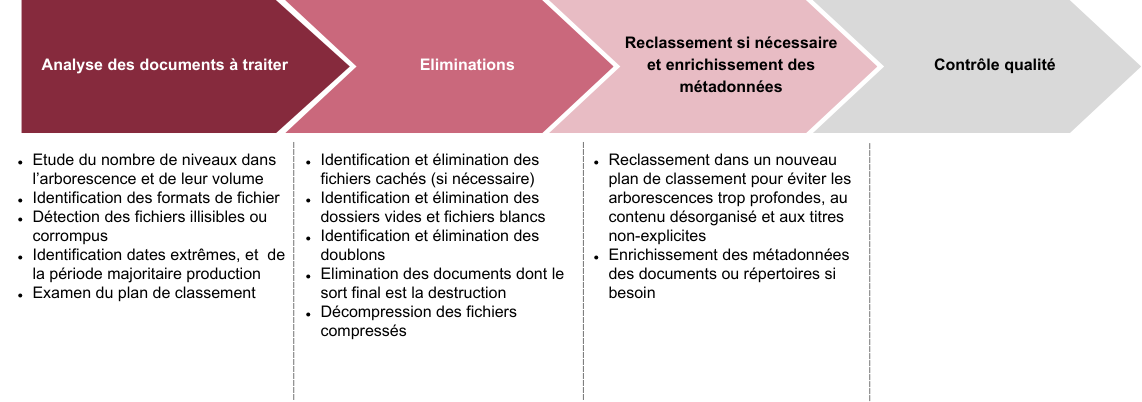
\includegraphics[width=\textwidth]{./media/image1.png}}
	\caption{Étapes de traitement des vracs numériques identifiées pendant le stage}
\end{figure}

\begin{figure}[h!]
	\centerline{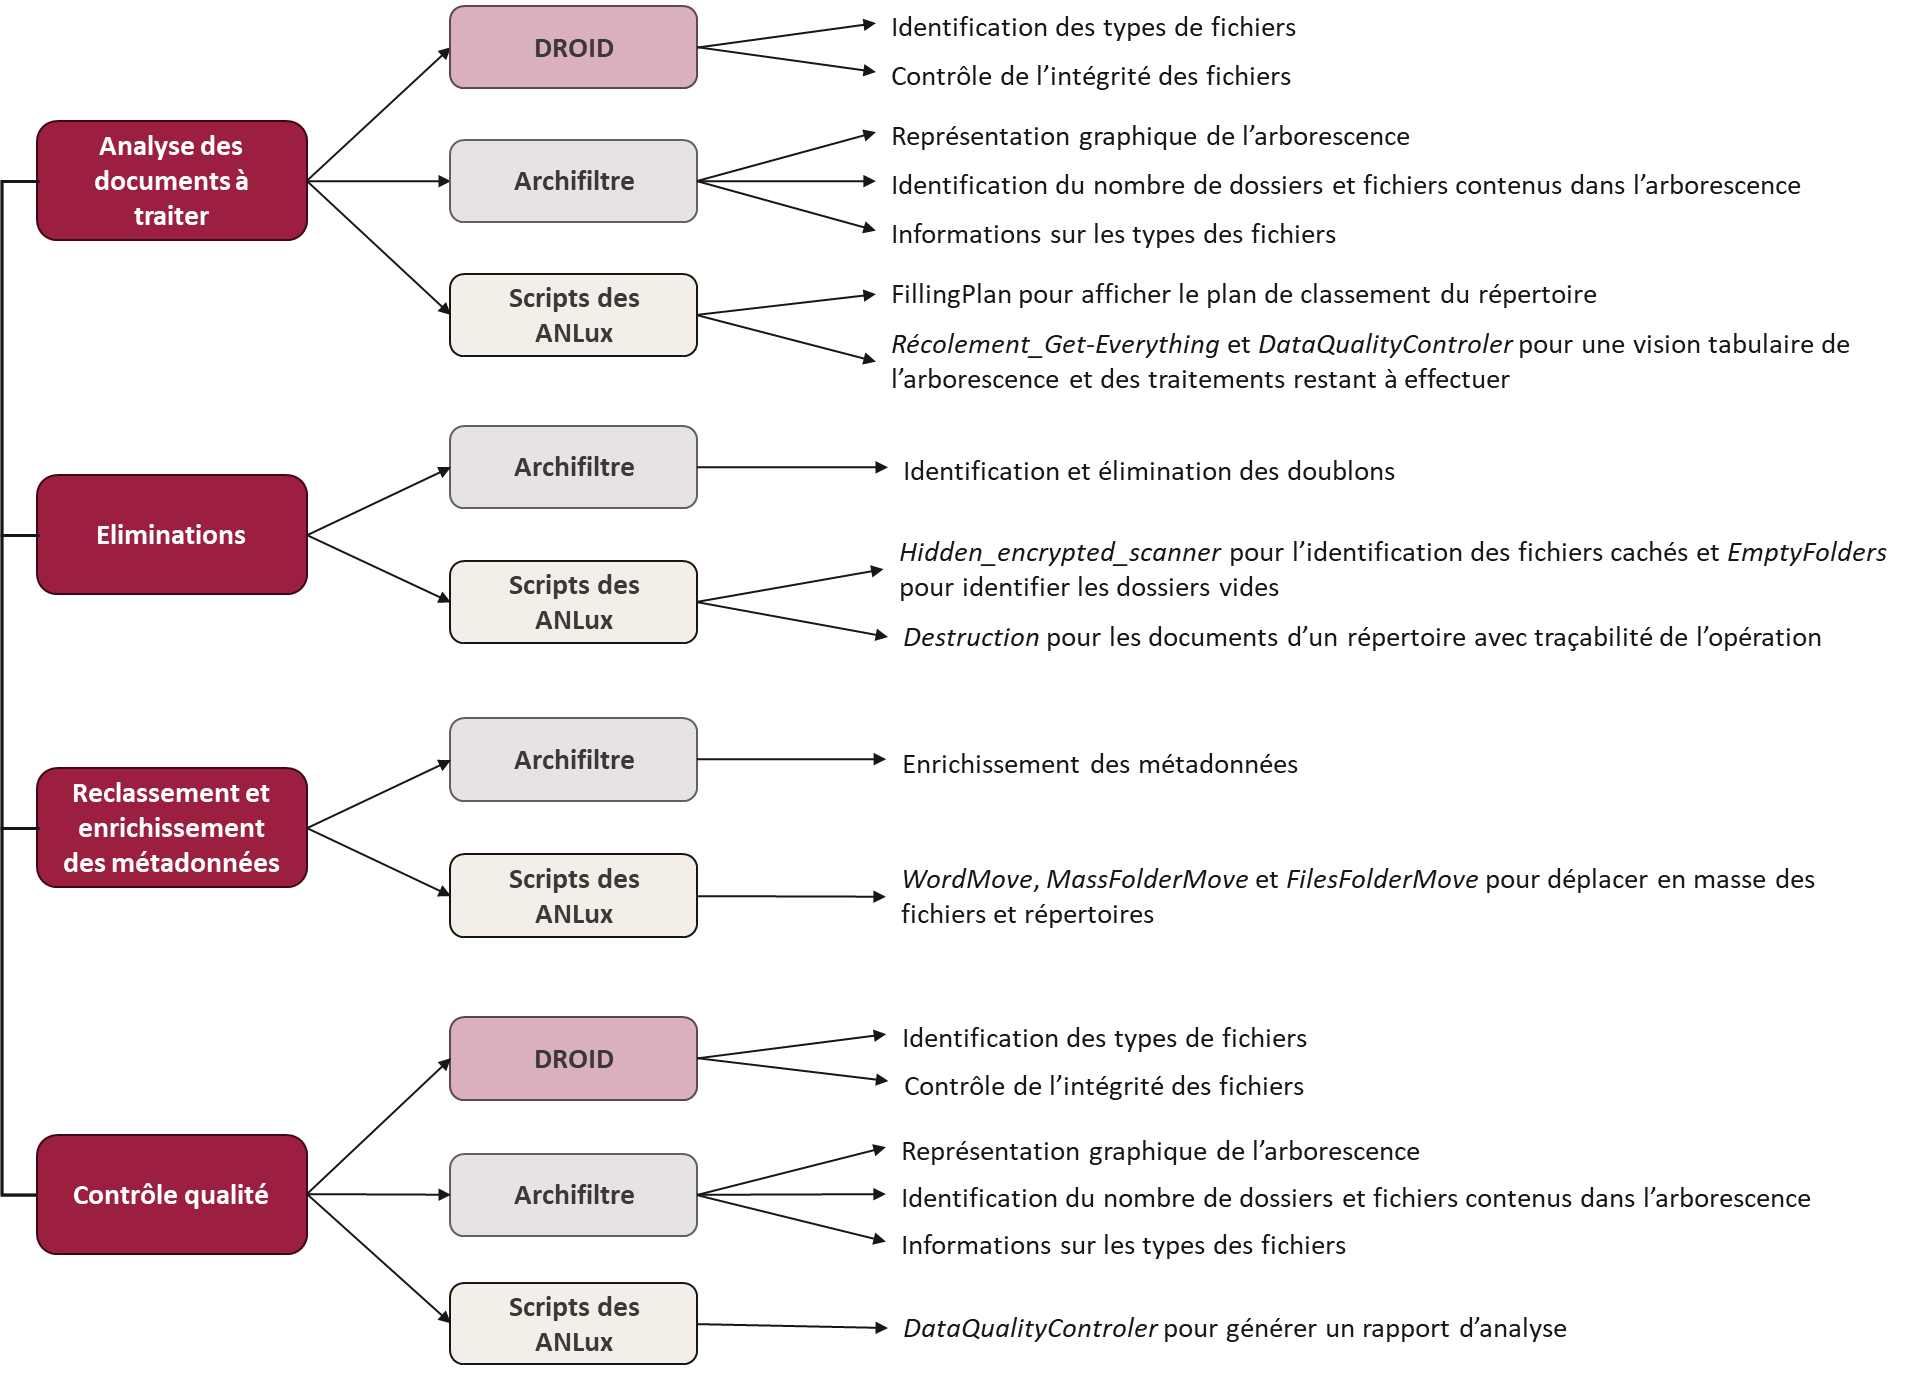
\includegraphics[width=\textwidth]{./media/image2.png}}
	\caption[note]{Moyens d'automatisation par étape de traitement de vracs numériques \footnotemark }
\end{figure}


La réalisation de l'inventaire vient après ces traitements. Une fois les
archives prêtes à être conservées, elles doivent être décrites et les
données sensibles doivent être repérées. L'ensemble de ce travail
nécessite du temps et des moyens, mais ils sont de moins en moins considérables grâce aux outils d'automatisation. 
L'article présentant le travail des ANLux en termes d'automatisation évoque qu'
 \enquote{en 2022, un vrac de 350 Go a nécessité près de 60 jours alors qu'en 2023, un vrac de 1,2 To n'en prenait que 20.\footcite{IA_porte}} 
En ce qui concerne l'inventaire, les
archivistes de la Chambre avaient calculé qu'il faudrait sept ans à
temps plein pour rédiger les inventaires de l'ensemble des fonds papier et numériques sans moyen d'automatisation. 
Un autre enjeu du traitement des archives numériques, au delà de sa complexité, est en effet leur masse. 
\footnotetext{N.B. D'après l'expertise des ANLux, les chiffres sur les nombres de fichiers sont à prendre avec vigilance, Archifiltre, Droid et Windows n'obtenant parfois pas les mêmes chiffres pour une même arborescence.}
Le numérique fait partie intégrante du fonctionnement des administrations. Des quantités
importantes de données sont dès lors produites. Le personnel de
l'administration n'a pas de vision claire de l\textquotesingle ampleur
des données générées et il est aisé de créer un nouveau document dans un
système ou bien de générer de nouvelles données. Le fonds du Service des
relations européennes et internationales et du protocole (SREIP), qui a
été choisi comme base de données pour la recherche et le développement
dans le cadre du projet InventAIre, contient par exemple 140 000
documents pour 80 000 répertoires. Il s'agit de l'arborescence complète
des fichiers du service contenus sur les serveurs. Un bénéfice de la
réalisation de l'inventaire des archives est de mieux s'y retrouver dans
ces documents en fournissant des titres et des descriptions des
différents répertoires.


Idéalement, une fois les vracs traités, la communication des documents doit
être assurée. C'est à ce moment que se pose la question de
l'identification données sensibles dans les documents. Il s'agit d'un
processus long qui demanderait à un ou une archiviste d'examiner chacun
d'entre eux. C'est un obstacle à une communication optimale des documents.
Ces archives dont l'accessibilité est empêchée par les défis liés aux
données sensibles ont été théorisées sous le nom de «~\textit{dark
archives}~».\footcite{baron_dark_2017}. D'après Jason Baron et
Nathaniel Payne, chercheurs américains et canadiens, la communication
des archives numériques nécessite un long travail d'identification des
données sensibles. Les administrations publiques sont en quête de
transparence mais l'accès à leurs archives serait menacé. Pour
automatiser le repérage des données sensibles, ils proposent plusieurs
solutions. L'utilisation d'\gls{REGEX} pour repérer des
informations confidentielles, telles que des numéros de sécurité sociale,
est une première solution, même si son efficacité est limitée. Le
recours au \emph{machine learning} est présenté comme une perspective
fructueuse. La \gls{clustering} automatique et le
\gls{deep} sont
envisagés\footcite{baron_dark_2017}. L'article date de 2017,
l'usage du \emph{machine learning} dans les archives en était à ses
débuts. L'architecture \emph{Transformer}, nouvelle manière de concevoir des
modèles d'IA ayant permis de rendre les modèles de langage plus rapides
et plus puissants et donc le développement des Grands modèles de
langage, a été proposée en 2017\footcite{vaswani_attention_2023}. Les auteurs avaient donc déjà
saisi les bénéfices des futurs grands modèles de \emph{deep learning}
pour le traitement des archives. Le \gls{cloud} est également évoqué comme une méthode
efficace pour faciliter le traitement automatique des données sensibles.
Il permet d\textquotesingle accéder à une puissance de calcul et de
stockage massive via des serveurs distants, par rapport à un
hébergement sur des ordinateurs en local. L'analyse des documents peut
alors être réalisée beaucoup plus rapidement et avec des outils plus
volumineux, comme des grands modèles d'intelligence artificielle.
L'usage du \emph{machine learning} pour automatiser la rédaction de
l'inventaire des ANLux, contenant des colonnes sur les données
sensibles, n'est donc pas sans fondement, ce type d'application a déjà
été pensé. Toutefois, pour que l'automatisation fasse réellement gagner du temps aux équipes, elle doit être précise.\newline

Ainsi, les défis auxquels sont confrontés les producteurs d'archives
publiques luxembourgeois sont nombreux, qu\textquotesingle ils soient
liés à la gestion des documents papier ou à la gestion des archives
numériques. Ces dernières posent des problèmes spécifiques liés à la
quantité massive de données à traiter et aux complexités techniques
associées à ce traitement. Pour relever ces défis, il convient
d\textquotesingle explorer des solutions innovantes, de tenter
d'automatiser des processus, et de tirer parti des pratiques développées
ailleurs. Ces défis peuvent
également être perçus comme des opportunités. Le fait de partir sur des
bases récentes permet d\textquotesingle expérimenter de nouvelles
approches. Cette situation rend les producteurs
d\textquotesingle archives plus ouverts à tester de nouveaux outils et à
initier des projets innovants, qui pourraient transformer la manière
dont les archives sont gérées à l\textquotesingle avenir.




		\chapter{Prérequis et points d’attention pour le pilotage de projets d’automatisation via l’IA dans les archives}

\subsection{Des besoins métier multiples mais des cas d'usage à préciser}

Les paragraphes précédents illustrent à quel point les besoins et possibilités en termes
d'automatisation sont nombreux chez les producteurs d'archives publiques.
Les services ont l'opportunité d'expérimenter avec l'IA. Il est plus aisé
d'obtenir des financements publics pour des projets qui utilisent des
technologies dans l'ère du temps. Les projets IA obtiennent d'autant
plus de financements dans le cadre de leur promotion par les états
mentionnée en première partie. Ce type de projets nécessite néanmoins une
réflexion approfondie en amont pour assurer un pilotage efficace et
garantir des résultats concrets.\newline

Tout d'abord, pour que ces projets impliquant du \emph{machine learning}
réussissent, ils doivent non seulement répondre à des besoins métier,
mais également avoir des cas d'utilisation bien précis. Le cas
d'utilisation ou cas d'usage est défini par Alistair Cockburn, expert en
\gls{agiles}, comme «~une description des séquences possibles
d\textquotesingle interactions entre un système en question et ses
acteurs externes, liées à un objectif particulier\footcite{cockburn_writing_2001}~» {[}Traduction libre{]}. L'informaticien suédois Ivar
Jacobson aurait été le premier à introduire des cas d'usage à la fin des
années 1960\footcite{cockburn_writing_2001}. C'est à partir des années
1980-1990 qu'ils ont été davantage formalisés. D'après Alistair
Cockburn, pour rédiger un cas d\textquotesingle utilisation efficace, il
faut commencer par définir clairement le périmètre du système et
identifier tous les acteurs et leurs objectifs. Il faut ensuite rédiger
le scénario de succès principal en décrivant chaque étape comme un
objectif atteint, puis ajouter les alternatives et les échecs possibles\footcite{cockburn_writing_2001}.
Il s'agit donc d'une modélisation de processus qui place les acteurs et
leurs interactions avec le système au centre. Les cas
d\textquotesingle usage sont d'une réelle importance pour les projets
IA. Ils permettent d\textquotesingle ancrer ces derniers dans des
réalités concrètes et de s\textquotesingle assurer que les solutions
développées répondent réellement aux besoins des utilisateurs finaux.
Sans cas d\textquotesingle usage bien définis, les initiatives IA
risquent de s\textquotesingle éparpiller et de ne pas apporter la valeur
ajoutée escomptée pour le métier. Les problèmes liés aux cas
d'utilisation sont parmi les cinq catégories de facteurs d'échec des
projets IA, avec les attentes irréalistes, les contraintes
organisationnelles, le manque de ressources et les problèmes techniques selon une étude réalisée par des chercheurs de
l'université de Reutlingen et un consultant de la société EXXETA en
2021\footcite{westenberger_failure_2022}. Une bonne spécification
de cas d'usage serait également un des éléments clés de la réussite
économique des projets IA dans le secteur privé d'après une autre étude
récente menée en Allemagne\footcite{grebe_artificial_2023}.
Les entreprises peineraient à faire évoluer les projets IA pilotes vers
des environnements de production. Les cas d'usage permettent de se
concentrer sur les points les plus complexes à traiter et
d\textquotesingle exploiter les opportunités de valeur ajoutée, au lieu
de se limiter à des projets réalisés sur des données parce qu'elles sont
facilement accessibles mais sans but précis. La validation du bon
fonctionnement d'un cas d'usage est une condition
pour le passage d'un projet pilote à un déploiement à plus grande échelle.
Les objectifs et les interactions avec les utilisateurs finaux doivent être clarifiés\footcite{grebe_artificial_2023}. Cette approche assure que les projets
répondent aux véritables besoins du métier. Il est en effet important de
noter que l'IA n'est pas la solution la plus efficace dans tous
les cas.\newline 

Une définition précise des cas d\textquotesingle usage permet en outre
une implication des équipes dès la genèse du projet, un élément clé dans
la \gls{changement}. En suivant une approche
similaire au \emph{design thinking}\footnote{Méthode de conception
	centrée sur l'utilisateur, qui le met parfois à contribution dans le
	processus de développement.}, où l\textquotesingle utilisateur final
est au centre du processus de conception, les cas
d\textquotesingle usage permettent de visualiser comment
l\textquotesingle IA peut s\textquotesingle intégrer dans les processus
actuels. Cela favorise son acceptation en tant qu\textquotesingle outil collaboratif~: la
machine doit compléter et accélérer le travail humain au lieu de le
remplacer. Cette idée est évoquée dans un article précédemment cité
intitulé «~Implementing AI in the public sector~»~: l'IA doit permettre
au personnel de se concentrer sur des tâches décisionnelles complexes et
la libérer des tâches répétitives. Au lieu de se concentrer sur l'idée
de remplacement des humains par l'IA, il est suggéré aux
acteurs publics de réfléchir à la manière dont l'IA augmentera les
capacités humaines et dont humains et machines peuvent
collaborer\footcite{mergel_implementing_2023}. Cette approche
collaborative constitue effectivement une stratégie pour atténuer les
craintes des personnes qui redoutent d\textquotesingle être remplacées
par l\textquotesingle IA, notamment dans un secteur où les recrutements
risquent de diminuer et les externalisations de se multiplier. Bien que
la sécurité de l\textquotesingle emploi soit généralement plus élevée
dans le secteur public, l\textquotesingle accent mis sur
l\textquotesingle intégration harmonieuse de l\textquotesingle IA permet
de rassurer le personnel en mettant en avant la complémentarité entre
les capacités de l'humain et de la machine. Les systèmes intégrant du
\emph{machine learning} sont presque constamment humanisés dans la
littérature. Le terme «~intelligence artificielle~» est déjà un résultat
de cet anthropomorphisme. Les prototypes d'automatisation sur les tâches complexes
n'atteignent pas les 100~\% de précision.
Il ne s'agit donc pas réellement d'une automatisation complète de
processus, mais l'IA serait une sorte d'agent qui réaliserait une partie
du travail au sein du processus, il s'agirait davantage d'une augmentation que d'une automatisation. En mettant des mots sur l'organisation de
cette collaboration homme-machine, l\textquotesingle efficacité des
outils IA pourrait donc se voir maximisée, et les inquiétudes des
équipes minimisées.\newline

Dans le cas du projet InventAIre, l'usage a été défini par l'équipe~:
l'outil développé a pour but de produire automatiquement des inventaires
d'archives au format \emph{Excel} d'après le modèle fourni par les
ANLux. Nous avons réalisé des diagrammes détaillant le
processus technique mis en œuvre par l'outil produit. Il faudrait
pousser ce travail plus loin en impliquant davantage les
utilisateurs, précisant leurs interactions avec le système. Pour
cela, la réalisation de diagrammes suivant des langages normés, tels que
l'UML\footnote{\emph{Unified Modeling Language}, un langage de modélisation
	standardisé utilisé en ingénierie logicielle pour visualiser,
	spécifier, concevoir, et documenter les éléments d\textquotesingle un
	système logiciel à travers différents types de diagrammes. Il aide à
	représenter les structures, les comportements, et les interactions
	d\textquotesingle un système de manière claire et compréhensible.},
est une possibilité à envisager. Le scénario précis d'utilisation de
l'outil gagnerait à être davantage défini. Il semble nécessaire de
clarifier comment la collaboration homme-machine se déroulera
concrètement : l'inventaire produit sera-t-il utilisé tel quel, avec un
processus de vérification en place, ou l'outil servira-t-il à accélérer
le travail de l'archiviste en fournissant un document pré-rempli que
celui ou celle-ci pourra ensuite compléter et ajuster ? Cette approche doit
également tenir compte des risques associés à la précision des résultats. Par exemple, les colonnes de l'inventaire concernant les descriptions et titres
présentent moins de risque en cas de manque  que celles
contenant les informations sur les données sensibles, qui nécessitent une
attention particulière. Un parallèle peut être tracé avec l'exemple des
voitures autonomes exposé dans l'article sur les causes des échecs des
projets IA~: il est dit que «~dans des cas d\textquotesingle utilisation
spécifiques, comme la conduite autonome, une faible tolérance aux
erreurs peut entraîner l\textquotesingle échec du projet. Ces cas
d\textquotesingle utilisation dépendent de prévisions et de résultats
précis et corrects, car une erreur peut avoir des conséquences
fatales\footcite{westenberger_failure_2022}.~» {[}Traduction libre{]}. Dans le cas du repérage
des données sensibles, si l'inventaire est réutilisé tel quel, sans
vérification, la tolérance aux erreurs sera faible et si le modèle de
\emph{machine learning} donne des taux d'erreur qui ne sont pas assez
proches de zéro, le projet sera un échec. Concernant la tolérance aux
erreurs, d'après Lise Jaillant et Arran Rees , «~le risque de
divulguer des données potentiellement sensibles doit être comparé au
risque de garder les archives confidentielles et inaccessibles\footcite{jaillant_applying_2023}~»
{[}Traduction libre{]}. Une précision inférieure à
100~\% peut être un risque choisi et mesuré par le service. Des
réflexions supplémentaires sur ces questions seront par conséquent à
mener en cas de poursuite du projet InventAIre. Les choix devront être
guidés par une analyse de risque approfondie, la définition d'un niveau
de précision acceptable et un processus rigoureux d'évaluation des
résultats produits par les modèles de \emph{machine learning} pour
vérifier qu'ils sont conformes à ce niveau de précision.
Si cette dernière n'est pas proche des 100\%, nous préconisons 
une vérification des inventaires par les archivistes au moins sur 
les colonnes de l'inventaire traitant les données sensibles avant 
leur mise à disposition pour le public.
\newline

La définition précise des cas d'usage revêt donc une grande importance
pour assurer la réussite des projets d\textquotesingle IA dans les
archives, car elle permet de clarifier les objectifs et
d\textquotesingle aligner les attentes tout en intégrant les besoins
réels des utilisateurs. Cette étape est interdépendante avec les
étapes de définition du périmètre et d\textquotesingle analyse des
risques. L'approche à adopter présente des différences par rapport à
la gestion des projets archivistiques traditionnels. Le notion de cas
d'usages vient du domaine de l'informatique. La gestion des projets doit
ainsi être réfléchie et adaptée pour une application de l'IA dans les
archives.



\subsection{Optimiser la gestion de projets IA dans les archives : réflexions et défis}


Avant de mettre en place des projets IA, les services d'archives
publiques doivent considérer les particularités de la gestion de projets
impliquant des outils basés sur le \emph{machine learning}. La gestion
de projet peut se définir comme l\textquotesingle organisation, la
planification et la coordination des ressources dans le but atteindre des
objectifs spécifiques dans un délai donné. La gestion de projet comme
outil managérial se serait rationalisée dans les années 1930 dans le
secteur public et aurait été théorisée en tant que modèle à la fin des
années 1950\footcite{garel_pour_2003}. Une bonne gestion de projet permettrait de mieux visualiser
et de maximiser les résultats. Différents outils et méthodes de gestion de
projet ont émergé. La plus connue est la méthode agile, popularisée
suite à la publication en ligne du \emph{Manifeste pour le développement
	agile de logiciels} en 2001\footcite{noauthor_manifesto_nodate}. Les
\gls{agiles} sont des méthodes de gestion de projet qui privilégient
l\textquotesingle adaptabilité, la collaboration et
l\textquotesingle itération dans le développement de produits. Elles se
basent sur des cycles de travail courts, nommés sprints, à l'issue
desquels les équipes évaluent et ajustent leurs priorités en fonction du
retour des acteurs du projet, en particulier des commanditaires ou
utilisateurs. Les avantages incluent une meilleure réactivité aux
changements, une bonne communication entre les acteurs et un produit
final davantage aligné sur les besoins réels des utilisateurs. 
Ces méthodes ne sont pas forcément éligibles à tout type de projet 
mais sont particulièrement adaptées aux projets informatiques car elles
 permettent de livrer rapidement des versions fonctionnelles d'un 
 produit et favorisent alors une amélioration continue en fonction 
 des retours de ses utilisateurs.


 La sociologue Camille Girard-Chanudet décrit la logique projet employée dans
la pseudonymisation automatique sur des documents par l'IA à la Cour de
Cassation comme s'inscrivant dans «~le cadre de la "transformation de
l'action publique"\footcite{girard-chanudet_travail_2023}~». Cette logique projet s'est
manifestée à la Cour de Cassation par l\textquotesingle intégration
d\textquotesingle une approche structurée autour
d\textquotesingle objectifs clairs, d'un produit minimum viable (MVP) et
d\textquotesingle un calendrier précis\footcite{girard-chanudet_travail_2023}. Cette
approche favorise non seulement l\textquotesingle efficacité, mais
s\textquotesingle inscrit également dans une volonté plus large de
modernisation et de digitalisation des services publics, conformément
aux objectifs de la «~transformation de l'action publique~». Cette
transition numérique a favorisé l'adoption de méthodes de gestion de
projet, notamment les méthodes agiles, au sein des administrations
publiques. Elles se sont souvent inspirées du secteur privé. Ces pratiques sont en effet
adoptées par les entreprises de services numériques travaillant pour le
secteur public. En France, un accent a été mis sur
l\textquotesingle innovation et le dynamisme avec, au cours des dix dernières années,
l\textquotesingle introduction de concepts comme les \enquote{entrepreneurs
d'intérêt général} (EIG), recrutés de manière régulière depuis 2017, et le
développement de « start-ups d'État ».
Dans le domaine archivistique, \emph{Archifiltre} est un exemple de
start-up d'État. L'objectif est de moderniser le service public,
d'améliorer la productivité et de favoriser l'innovation. Au Luxembourg,
la création du \emph{GovTech Lab} vise à soutenir
l\textquotesingle innovation au sein de l'État. Ainsi, les états
encouragent l'innovation en adoptant des méthodes courantes et
performantes dans le secteur privé, ce qui explique la popularité
croissante de ces pratiques dans le secteur public. À la Chambre des
Députés, le service Technologies de l'information (TI) a recruté quatre chefs
de projet depuis 2022, s\textquotesingle inscrivant dans cette même
dynamique de modernisation. Les chefs de projet se multiplient aussi
dans les autres administrations publiques.\newline

En ce qui concerne les projets archivistiques, en 2018, Cyndi Shein,
Hannah Robinson et Hana Gutierrez ont proposé d'introduire les principes
agiles dans leur gestion, soulignant que les
archivistes gèrent des projets mais n'accordent pas suffisamment
d'attention à la théorie de la gestion de projet\footcite{shein_agility_2018}. À la Chambre des Députés, les
projets archivistiques sont formalisés de la même manière que ceux des
autres domaines, avec des noms et des identifiants, c'est le cas du
projet InventAIre qui porte l'identifiant P1134. Un chef de projet de
l'équipe du service TI a été désigné pour le suivre, et les outils des
méthodes agiles issus de la gestion informatique ont été utilisés. Un
diagramme de Gantt\footnote{Planning des tâches à accomplir montrant leur durée et leur chevauchement sur une échelle de temps.} a été réalisé. Des comités de projet et de pilotage
ont été organisés pour suivre l'avancement et valider différentes
décisions. D'autres outils
de gestion de projet qui sont quant à eux spécifiques à l'informatique,
comme la méthode MoSCoW\footnote{Hiérarchisation des objectifs de développement d'un outil en quatre catégories : \textit{Must have} (minimum à développer), \textit{Should have} (fonctionnalités que l'on devrait développer mais non prioritaires), \textit{Could have} (pourrait avoir en mettant beaucoup d'efforts), \textit{Won't have} (hors périmètre).}, ont été employés pour hiérarchiser les
fonctionnalités de l'outil à produire. Ces outils ont largement contribué aux succès.


\begin{figure}[h!]
	\centerline{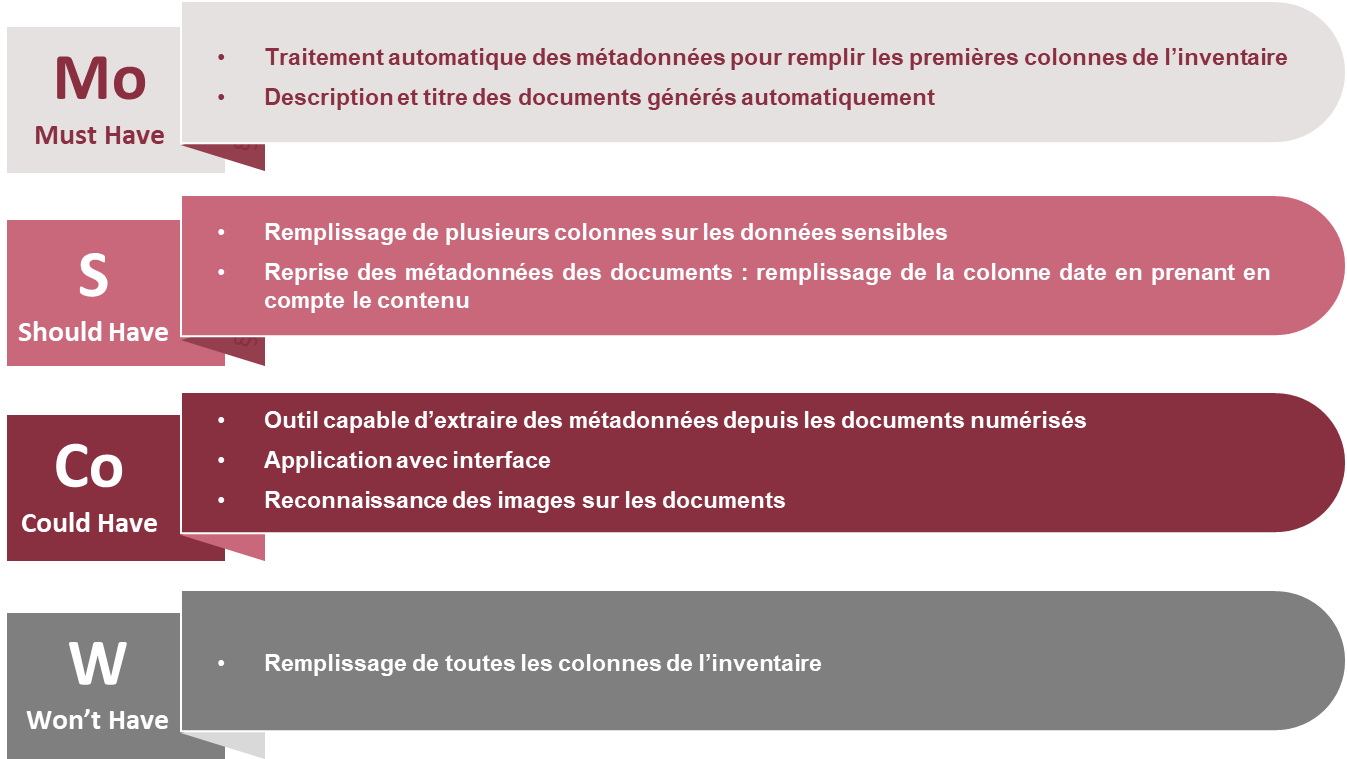
\includegraphics[width=\textwidth]{./media/image3.png}}
	\caption{Hiérarchisation des fonctionnalités à produire (MoSCoW) }
\end{figure}



Cette hiérarchisation a permis la réalisation du minimum requis. Lorsque
des difficultés sont apparues, les fonctionnalités non prioritaires ont
été mises de côté. Le projet InventAIre a ainsi démontré l'importance de
l'utilisation de méthodes de gestion de projets informatiques et d'une
bonne définition du périmètre. En effet,
l\textquotesingle ampleur des ressources et du personnel nécessaires à
la réussite des projets IA est souvent sous-estimée. Camille Girard-Chanudet évoque en parlant du
système basé sur le \emph{machine learning} développé à la Cour de Cassation
que «~loin de l'image d'autonomie généralement associée à ce type de
dispositifs techniques, la charge de travail humain dans le
fonctionnement d'un tel outil est conséquente~: celui-ci mobilise au
quotidien plus de 20 personnes à la Cour\footcite{girard-chanudet_travail_2023}~».
Le travail d'annotation des données à pseudonymiser demande en effet
beaucoup de ressources humaines. L\textquotesingle annotation en
\emph{machine learning} consiste à étiqueter ou décrire des données
(comme des images, du texte ou des sons) pour que les algorithmes
puissent apprendre à reconnaître et à traiter ces informations de
manière autonome. Cette étape est obligatoire pour le développement de modèles de \emph{machine
	learning} maison. En plus des personnes pour
réaliser les annotations, il faut également mobiliser du personnel pour
la gestion de projet et pour le développement de l'outil. Dans le cas du
projet InventAIre, nous n'avions pas le temps d'annoter des données
suffisantes pour développer un modèle d'IA en quatre mois de stage. Il
était donc impossible d'entraîner un modèle d'\gls{supervisé}. Nous avions ainsi 
comme option
l'\gls{non-supervisé} ou le choix d'un \gls{pré-entraîné}. Nous avons pu adapter le périmètre et
l'approche. Néanmoins, même dans le cas de l'usage de modèles
pré-entraînés, les investissements en temps et en ressources humaines
restent non-négligeables. Il faut par exemple prévoir une longue période
de tests afin de choisir le bon \gls{pré-entraîné} et mobiliser du personnel pour évaluer les résultats produits par l'IA. Pour un projet de
\gls{chatbot} à la BNL, d'après Yves Maurer, en charge du projet, le
«~plus chronophage a été de tester plusieurs alternatives pour chaque
brique du projet : des modèles de langage ouverts, un autre créé par
un groupe de recherche, celui de Meta et de Google\ldots \footcite{noauthor_comment_nodate}~». Dans le
	cadre de notre projet la période de tests a pris environ deux mois  avec une seule personne mobilisée. 

D'autres différences notables existent entre les projets archivistiques
et ceux impliquant l\textquotesingle IA. L\textquotesingle approche
cyclique est encore plus importante pour l\textquotesingle IA~: la
précision des outils produits doit
être évaluée à chaque étape. Les cycles sont de tailles différentes. Les
étapes de test et de réflexion sont assez lentes. Le code de l'outil en
lui-même a été assez rapide pour le projet InventAIre. Les périodes
d'évaluation et de reprise de l'outil en fonction des résultats de ces
dernières sont quant à elles longues et on ne peut pas prévoir leur nombre
d'itérations.\newline

\begin{center}
	Estimation du temps sur les différentes \enquote{tâches IA} pendant le projet
\end{center}

\begin{longtable}{|p{0.45\textwidth}|p{0.5\textwidth}|}

    \tableheader{Tâche}{Estimation de temps}
	
	Définition du périmètre et de l'approche & 15\% \\
	\hline
	Tests pour le choix d'un modèle & 40\% \\
	\hline
	Code sur l'intégration du modèle & 10\% \\
	\hline
	Prompt-engineering & 15\% \\
	\hline
	Évaluation de l'outil\up{*} & 15\% \\
	\hline
	Autre & 5\% \\
	\hline
\end{longtable}
\begin{noindentpar}
	\up{*}\footnotesize{Ce temps a été réduit parce que le stage se terminait, l'évaluation doit idéalement être plus longue pour être davantage pertinente et mener à des reprises de l'outil}
\end{noindentpar}\\

Un inconvénient de ces méthodes agiles est le temps que la gestion de
projet exige. Pendant notre stage, les tâches de gestion de projet ont
représenté environ 15 \% de notre temps\footnote{Un diagramme de répartition du	temps est consultable dans la note méthodologique en annexe.}, incluant
la définition du périmètre et du calendrier, la préparation et la tenue
des réunions ainsi que la rédaction des comptes rendus. Pour des
projets de plus grande envergure, il est essentiel de séparer les
fonctions de recherche et développement de celles de gestion de projet
entre plusieurs personnes. La constitution d'une équipe projet
favorisant la collaboration entre archivistes et spécialistes des
technologies de l'information est nécessaire.

Enfin, ces projets nécessitant d'importants investissements humains et
financiers et l'intelligence artificielle étant un nouveau territoire à
explorer pour les institutions publiques, il est nécessaire de commencer
par des projets pilotes, des preuves de concept (POC) ou des études de
faisabilité avant de se lancer dans de grands projets. La plupart des
institutions suivent ces recommandations. C'est notamment le cas de la
BNL (Bibliothèque nationale du Luxembourg) qui a lancé plusieurs projets pilotes ces dernières années, dont un
projet d'amélioration de la transcription par \gls{OCR} et un projet de \emph{chatbot} permettant la recherche
dans les fonds de presse numérisés\footcite{noauthor_comment_nodate}. À la Chambre des Députés, le projet InventAIre constitue
la première étape d\textquotesingle un processus plus large. La phase
suivante consiste à réaliser un POC, à partir duquel un outil serait
développé et mis en production.

L\textquotesingle intégration des méthodes de gestion de projet, en
particulier les approches agiles, est par conséquent une composante de la réussite des
projets IA dans le secteur des archives. Le projet InventAIre illustre
comment une gestion efficace, une collaboration interdisciplinaire et
une approche itérative permettent d'être en mesure de naviguer avec succès entre les défis spécifiques à l\textquotesingle IA.

\subsection{Gestion des risques et défis éthiques des systèmes	basés sur le \emph{machine learning}}

Les risques liés à l\textquotesingle intelligence artificielle, en
particulier dans le domaine des archives, sont nombreux, allant bien
au-delà des simples considérations légales facilement identifiables.
Outre les enjeux juridiques, il existe des risques sociaux et
éthiques, qui seront détaillés dans le début du chapitre 8. Face à ces défis,
une analyse de risques est à prévoir. A la Chambre des Députés, une
mitigation des risques a été réalisée en amont en collaboration avec le
\emph{DPO (data protection officer)} et le Responsable sécurité des
systèmes informatiques. C'est ainsi qu'il a été décidé qu'il n'était pas
question de transmettre des données à un tiers, nous avons ainsi dû
travailler avec des modèles pré-entraînés hébergés localement sur nos
ordinateurs, et non dans le \emph{cloud}. Cela n'est pas sans conséquence. Ceux
que nous pouvions faire tourner étaient en effet moins précis que les
grands modèles hébergés dans le \emph{cloud} et très volumineux sur nos
machines, donc relativement lents. Les autres risques identifiés
concernaient un mauvais remplissage de l'inventaire, contenant des biais
ou \gls{hallucination}s. Les titres et descriptions en texte libre générés par
des grands modèles de langage peuvent facilement contenir des
erreurs, des informations non pertinentes ou des hallucinations. Au
contraire l\textquotesingle IA pourrait aussi invisibiliser certaines
informations jugées non pertinentes, entraînant une perte de données
essentielles. Enfin, la gestion des données sensibles nécessite une
attention particulière : une erreur dans ces données pourrait avoir des
conséquences graves. Face à ces risques, il a été décidé qu'un contrôle
qualité rigoureux serait effectué. 
Un tableau contenant les risques et contre-mesures identifiés au début du projet se trouve dans la partie 1.1.2. de la note méthodologique en annexe.\newline

Le chercheur James Lappin propose dans sa thèse intitulée «~The science
of recordkeeping systems -- a realist perspective~», une distinction
entre les applications «~low-stakes~» (à faible enjeu) et
«~high-stakes~» (à fort enjeu) de l'IA dans le domaine du \emph{record
	management}. Les applications « low-stakes » incluent
l\textquotesingle utilisation de l\textquotesingle IA pour classer les
résultats de recherche, personnaliser les recommandations, visualiser
les contenus ou extraire des entités, sans altérer les règles
d\textquotesingle accès ou de conservation des documents. En revanche,
les applications « high-stakes » impliquent des décisions aux
conséquences irréversibles, qui modifient les règles de conservation ou
d\textquotesingle accès aux documents, par exemple via des éliminations ou
l\textquotesingle octroi de certains accès\footcite{lappin_science_2024}. Les autres projets
d\textquotesingle intelligence artificielle mis en place dans le domaine
des archives et des bibliothèques au Luxembourg sont majoritairement des
projet «~low-stakes~». C'est par exemple le cas des \emph{chatbots} de la
Bibliothèque Nationale du Luxembourg (BNL) et du Parlement européen
mentionnés précédemment, qui permettent une recherche dans des documents
publics. Quant aux scripts générés par IA des ANLux, ils ont vocation à être
partagés, c'est aussi une utilisation avec moins de risques, car sans données confidentielles. 

Le projet
InventAIre est précurseur en termes d'application
«~high-stake~» de traitement automatique d'archives par IA. Il a ainsi constitué
une occasion de tirer plusieurs enseignements précieux concernant la
gestion des risques et leur atténuation. D\textquotesingle abord, il est
apparu particulièrement intéressant d\textquotesingle impliquer divers
acteurs dans le processus, tels que le responsable de la sécurité des
systèmes informatiques (RSSI) et le \emph{data protection officer} (DPO). Ces experts dans leur domaine
apportent des compétences spécifiques complémentaires à celles des
archivistes et des informaticiens. De plus, nous avons cherché à
impliquer le plus possible l'humain. C'est le concept de l'«~Human in
the loop~»~: l\textquotesingle humain a été intégré dans le processus de
développement et d\textquotesingle évaluation de l\textquotesingle IA.
Cela est particulièrement pertinent et à développer dans le cadre des
sprints agiles mentionnés précédemment, où chaque étape du développement
était validée par des retours humains. Cette méthode contribue non seulement à une meilleure
qualité des résultats, mais facilite également
l\textquotesingle instauration d\textquotesingle une meilleure confiance
des différents acteurs impliqués envers l'outil développé. Cette dernière facilite la \gls{changement}.
L\textquotesingle analyse des risques a joué un rôle dans la
construction de cette confiance en garantissant que chaque décision
prise soit justifiée. Cela a permis de créer un cadre sécurisé et le
plus transparent possible, favorisant ainsi l\textquotesingle adoption
et l\textquotesingle acceptation de l\textquotesingle IA dans un domaine
aussi sensible que celui des archives.

Les projets d'intelligence artificielle dans le domaine des archives
publiques offrent des perspectives prometteuses, mais ils posent
également des défis importants. Avant d'initier de tels projets, il convient
d'assurer une analyse des risques de manière proactive. Les exigences
éthiques et techniques sont nombreuses. Les besoins et usages doivent
être clairement identifiés et la gestion de projet réfléchie. \newline

En conclusion de ce chapitre, nous pouvons dire que les producteurs d\textquotesingle archives publiques luxembourgeois font
face à de nombreux défis qui, paradoxalement, offrent des opportunités
d\textquotesingle innovation et d\textquotesingle expérimentation. Un
contexte favorable au Luxembourg et en Europe encourage
l\textquotesingle implémentation de projets IA dans le secteur public
avec des ambitions élevées. Cependant, avant de lancer de tels projets,
des réflexions sur les prérequis en termes de pilotage sont à mener. Une
fois ces réflexions approfondies, les projets IA pourront aboutir à des
résultats et avoir des apports concrets pour les services
d\textquotesingle archives publics.	
		
	\part{Les apports des projets IA dans les archives :  perspectives, état des lieux et synergies}
		\chapter{Des solutions légères de \emph{machine learning} pour les archives}

\subsection{\gls{TAL} pour la classification~: \emph{clustering} et \gls{topic}}

Le premier travail effectué dans le cadre du stage a été de tester
plusieurs moyens de remplir les différentes colonnes de l'inventaire.
Nous avons commencé par tester des algorithmes légers d'\gls{non-supervisé}. 
L'apprentissage non supervisé est une technique
d\textquotesingle apprentissage qui permet de découvrir des structures
ou des modèles dans des données non étiquetées, sans intervention
humaine pour guider la machine. L\textquotesingle objectif est de
révéler des relations ou des regroupements intrinsèques entre les
données. Avant d'utiliser des grands modèles pré-entraînés, il est
important d'étudier ce qu'il est possible de faire avec des moyens
techniques plus légers. Le \gls{TAL} est
une discipline ancienne. Les premières recherches auraient été menées aux débuts
de l'informatique, dès les années 1940\footcite{poibeau_traitement_2014}.
L'article le plus ancien détaillant les potentiels usages du TAL, ou
\gls{NLP} dans les archives que nous ayons trouvé date de 1998 et
a été publié dans la revue \emph{The american archivist}\footcite{dooley_encoded_1997}.
Un rapport plus ancien de l'UNESCO intitulé «~Regional Training Centre
for Archivists, Accra: Africa - (mission). Project findings and
recommendations~» et publié en 1981, évoque l'idée qu'«~en tant que
banques de données de documents originaux, les archives ont beaucoup en
commun avec les bibliothèques et les centres de documentation, et
doivent de plus en plus utiliser des techniques automatisées de
traitement des données, de recherche et d\textquotesingle exploitation
de l\textquotesingle information, de résumé,
d\textquotesingle indexation et de diffusion~\footcite{unesco}~» {[}Traduction libre{]}. Le rapport n'évoque pas
directement le \gls{TAL} mais les \enquote{techniques automatisés} évoquées en
découlent. La théorisation de l'usage du TAL dans les archives date donc
au moins des années 1980. L'idée a eu le temps de mûrir en plus de
quarante ans, et les technologies de s'améliorer.

Dans le cadre du projet InventAIre, nous avons commencé par expérimenter
à l'aide d'algorithmes de classification automatique. L'usage de petits
algorithmes de TAL par rapport à des grands modèles pré-entraînés a
effectivement pour avantage de réduire les besoins en ressources
informatiques, de diminuer le temps de calcul et
d\textquotesingle éviter qu\textquotesingle un inventaire prenne trop de
temps à se générer. La classification automatique est une technique
d\textquotesingle apprentissage automatique qui consiste à générer
automatiquement des regroupements d'objets en fonction de leurs
caractéristiques. Pour que l'algorithme de classification puisse
regrouper automatiquement les documents, une représentation mathématique
de ces documents doit au préalable avoir été générée, c'est l'étape de
\gls{vectorisation}. Nous avons ainsi vectorisé les textes de chaque document.
Nous avons utilisé la méthode TF/IDF (\emph{Term Frequency-Inverse
	Document Frequency}). 

\begin{figure}[!h]
	\centerline{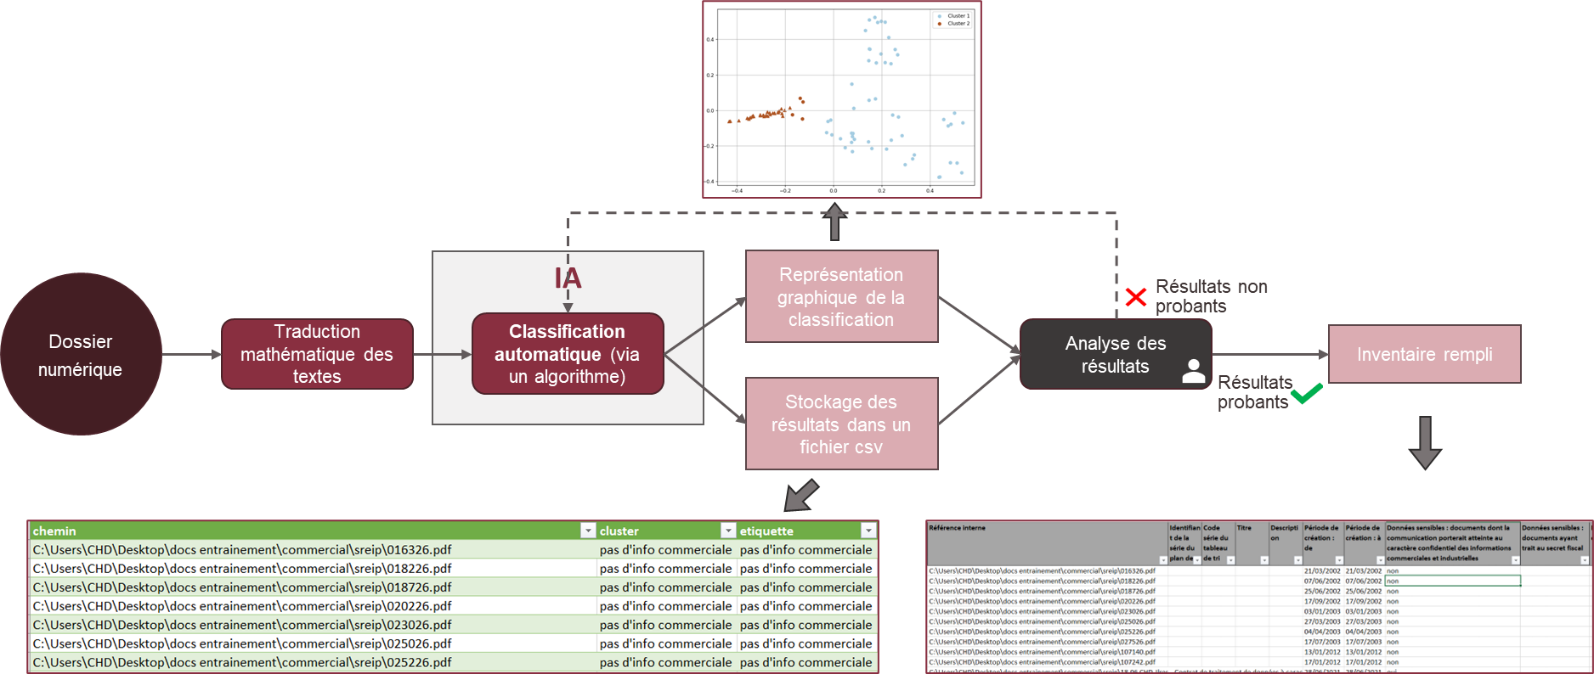
\includegraphics[width=\textwidth]{./media/clustering.png}}
	\caption{Exemple de processus de classification automatique : Clustering sur des documents contenant des informations à caractère commercial}
\end{figure}

Il y a plusieurs méthodes de vectorisation. TF/IDF
consiste à représenter un texte par un vecteur dont les composantes sont
les fréquences des mots dans le document, pondérées par leur importance
dans l\textquotesingle ensemble des documents. Cela met en
évidence les mots qui ont le plus de poids dans chaque document. Nous
avons également défini des \gls{stop-words}, qui sont des mots très
courants dans une langue ou dans le corpus de document, tels que « le »,
« la », « les », etc. qui n\textquotesingle apportent pas
d\textquotesingle information significative pour la classification. En
les éliminant, nous pouvons améliorer la précision de cette dernière.
Notre liste de \gls{stop-words} comportait les mots les plus fréquents
de la langue française et les mots du champs lexical de la législation,
qui se retrouvent dans la plupart des documents. Nous avons également
ignoré les chiffres qui se trouvaient dans les textes. Les vecteurs
obtenus sont des représentations numériques des documents, sous la forme
de tableaux dont chaque valeur correspond à
l\textquotesingle importance d'un mot dans le document.

Une fois ces vecteurs réalisés, il est possible de calculer le texte
le plus proche d'un autre, d'étudier les mots qui ont le plus de
poids pour les ajouter dans les \emph{stop words} s'ils ne sont pas pertinents,
ou d'afficher des groupes de documents les plus proches afin
d'identifier d'éventuels sujets. Après cette étape de vectorisation,
nous avons travaillé sur la classification des documents en appliquant
un algorithme de classification automatique nommé \emph{k-means}. Nous
sommes parvenue, après plusieurs essais, à créer des groupes de
documents à propos d'affaires juridiques et d'ordre commercial
(factures, contrats). Cette méthode était dans une certaine mesure
pertinente pour l'inventaire. Nous étions en mesure de détecter des
documents qui remplissent la colonne «~affaires portées devant des
instances juridictionnelles, extra-judiciaires ou disciplinaires~» et la
colonne «~informations commerciales ou industrielles~». Toutefois, les
textes dans lesquels la mention de ces informations était plus subtile se voyaient
ignorés. Par exemple, un rapport mentionnant de manière implicite une
affaire juridique, sans utiliser de termes spécifiques, passait
inaperçu. Inversement, une loi ou un document issu d'une question
parlementaire sur la justice, donc des documents publics, étaient
détectés comme faisant partie des documents sur des affaires
juridictionnelles. Le multilinguisme pose également problème. Même si la
langue de l'administration parlementaire est le français, le Luxembourg
a trois langues officielles : le luxembourgeois, le français et
l'allemand. De plus, nous avons travaillé sur un fonds relatif aux
relations internationales, ce qui impliquait un certain nombre de
documents en anglais. Il aurait fallu répéter l'ensemble du
processus dans ces quatre langues. Cette méthode n'a donc pas été
choisie pour remplir l'inventaire. Néanmoins, nous en avons retenu les
avantages analytiques des différents tests. Nous avons en effet
expérimenté la méthode avec des nombres différents de \emph{clusters} à
produire par l'algorithme, c'est à dire de groupements de documents
générés automatiquement. Un ensemble de paramètres est modifiable dans
l'algorithme de classification. L'algorithme
\emph{k-means} génère un nombre k
prédéfini de \emph{clusters}, en assignant chaque point au cluster dont il est
le plus proche du centre (centroïde), lui-même déterminé à partir de la
moyenne des coordonnées des points du \emph{cluster}. À chaque itération, nous
tentions de comprendre ce qui liait les documents regroupés. Nous avons
pu en dégager des thèmes, des types de documents et identifier les
différentes langues dans le fonds étudié, puisque les documents se
regroupaient aussi par langue. Ces expérimentations de classification
ont donc constitué une phase productive d'analyse du contenu du fonds.
On pourrait imaginer cette expérimentation comme partie intégrante de la
première étape des pré-traitements de l'archivage numérique, qui
consiste à étudier comment est constitué le fonds, notamment pour
visualiser ce qui est à éliminer. Les techniques de \gls{TAL} sont expérimentées dans 
d'autres projets dans cette même optique analytique. Par exemple, l'application Pêle-mél 
fournit un outil d'analyse des messageries grâce à un système de classification automatique\footcite{noauthor_bilan_nodate}.\newline

D'autres méthodes de classification automatique existent. Plusieurs ont
été testées par des chercheurs indiens sur des jeux de données
d'articles de presse et de critiques de films. Leur objectif était
d'analyser les résultats produits par les différentes méthodes sur des
longs documents\footcite{wagh_comparative_2021}. Dans
cette étude, dix méthodes différentes ont été essayées pour classer
automatiquement des textes longs. Certaines utilisent des modèles de
langage déjà entraînés sur de grandes quantités de texte,
qu\textquotesingle on adapte ensuite à la tâche spécifique de tri des
documents, comme les méthodes \emph{ULMFiT} et \emph{USE (Universal
	Sentence Encoder)}. D\textquotesingle autres s\textquotesingle appuient
sur des réseaux neuronaux, un type de modèle inspiré du cerveau humain,
qui analysent les mots dans l\textquotesingle ordre où ils apparaissent
et utilisent des mécanismes d\textquotesingle attention pour se
concentrer sur les parties les plus importantes du texte. Il y a aussi
des techniques plus classiques, qui comptent la fréquence des mots et
les pondèrent en fonction de leur importance pour le document, comme
\emph{TF/IDF}, que nous avons utilisé, adopté dans l'étude avec l'algorithme de classification \emph{Naive Bayes}. Une
méthode hiérarchique a également été testée, analysant
d\textquotesingle abord les mots, puis les phrases, pour comprendre le
texte dans son ensemble\footcite{wagh_comparative_2021}. Les méthodes de
classification automatique sont donc très diverses. Les résultats de
l'étude montrent que les gros modèles pré-entraînés tendent à offrir de
meilleures performances. Cependant, pour la plupart des jeux de données,
des modèles plus simples\footnote{Ex~: les embeddings de GloVe ou les
	réseaux LSTM peu profonds} peuvent fonctionner avec une perte minimale
en précision.

Les modèles pré-entraînés testés dans le cadre de l'étude sont
\emph{BERT} et \emph{DistilBERT}. Il existe en effet depuis quelques années des moyens
plus précis de vectoriser des documents que les calculs mathématiques de
méthodes comme TF/IDF. Il est possible de réaliser une \gls{vectorisation} qui
aurait une valeur sémantique grâce aux \gls{embeddings}
des grands modèles pré-entrainés tels que les \gls{LLM}). Contrairement à des méthodes comme TF/IDF, ces \emph{embeddings}
capturent la signification contextuelle des mots et rapprochent les
termes ayant des significations similaires dans un même espace
vectoriel. Ces représentations sont générées par des grands modèles de
langage entraînés sur de vastes corpus de textes, ce qui leur permet
d'appréhender des relations complexes entre les mots et
d\textquotesingle offrir une compréhension plus fine et plus nuancée du
contenu sémantique des documents. Ils gèrent également le
multilinguisme lorsqu'ils sont entraînés sur des corpus en plusieurs langues.
Des exemples de modèles d'\emph{embeddings} sont ceux de \emph{BERT},
développé par Google, ainsi que ceux des \gls{LLM} tels
que \emph{GPT-3} et \emph{GPT-4} par \emph{OpenAI}, ou \emph{LlaMa}
\emph{2} par \emph{Meta}. Une autre étude a été réalisée par des
chercheurs et des chercheuses norvégiens pour tester l'efficacité de
différentes méthodes de vectorisation avec de la classification pour
regrouper des articles de presse à propos de mêmes
événements\footcite{tarekegn_large_2024}.
Les meilleures performances étaient obtenues avec des \emph{embeddings} de
\emph{LLM}, puis ceux de \emph{BERT}, suivis par les algorithmes plus
légers et classiques comme \emph{TF/IDF} et \emph{GloVE}\footnote{Technique d'apprentissage automatique pour créer des représentations vectorielles d'entités textuelles en capturant des relations sémantiques entre mots à partir de leurs co-occurrences dans un corpus de texte}
\emph{(Global Vectors for Word Representation)}\footcite{tarekegn_large_2024}.
L'inconvénient principal de ces gros modèles est leur exigence en
puissance de calcul, nécessitant souvent des équipements spécialisés
comme des cartes graphiques (\emph{GPU}). Pour répondre à ce défi, des
versions optimisées des grands modèles de langage ont été développées.
Par exemple, \emph{DistilBERT} est une version allégée de \emph{BERT}
qui est 40 \% plus petite, fonctionnerait 60 \% plus rapidement mais qui
conserverait environ 95 \% des performances du modèle
complet\footcite{noauthor_distilbert_nodate}.
Ce type de modèles n'a pas été testé dans le cadre du projet
\emph{InventAIre}. Nous avons principalement utilisé les grands modèles
de langage pour la génération de texte, sans tester leurs
\emph{embeddings} pour des tâches de classification. Il pourrait être
intéressant de comparer leurs performances avec celles de la méthode
\emph{TF/IDF} sur des documents d'archives pour voir à quel point ils
sont davantage précis. La fourniture de données annotées peut
également améliorer significativement les performances des algorithmes,
il s'agit dans ce cas d'un \gls{supervisé}. Un projet mené par
des chercheurs brésiliens et américains sur la classification
automatique de documents contenant des secrets d'État a par exemple
montré des résultats prometteurs, avec une précision de 90~\% et environ
11~\% de faux positifs\footcite{souza_using_2016}.
Avec de grandes quantités de données, leur méthode pourrait être
applicable au remplissage automatique de l'inventaire des ANLux.
\newline

Une autre perspective réside dans l'extraction de groupes de mots
significatifs à partir de groupements de documents. C'est le concept du
\gls{topic}. Cette méthode permet
d\textquotesingle identifier des thèmes ou sujets sous-jacents dans un
ensemble de textes en regroupant des mots qui apparaissent fréquemment
ensemble. La technique la plus couramment utilisée pour le \emph{topic
	modelling} est \emph{LDA} (\emph{Latent Dirichlet
	Allocation})\footcite{velonis_topic_2022}. 
	\emph{LDA} fonctionne en attribuant chaque document à une
combinaison de sujets et en représentant chaque sujet comme une
distribution de mots. De la même manière qu'avec
l\textquotesingle algorithme \emph{k-means},
l\textquotesingle utilisateur doit définir au préalable le nombre de
groupes, donc le nombre de sujets souhaités. \emph{LDA} distribue alors
les documents et les mots entre ces sujets de manière à maximiser la
cohérence sémantique des groupes formés. Cela permet de dégager les
thèmes principaux abordés dans un corpus de manière automatisée, et sert
ainsi à l\textquotesingle analyse de grands corpus de texte.

Ces méthodes de TAL peuvent fournir des résultats mais nécessitent une série de tests et d\textquotesingle évaluations
pour sélectionner la méthode la plus appropriée, ce qui peut rapidement
devenir déroutant. Pour automatiser une tâche complexe, comme la
rédaction d\textquotesingle un inventaire, avec des ressources limitées,
il est souvent nécessaire d\textquotesingle utiliser une combinaison de
plusieurs méthodes ou modèles. Pour obtenir une bonne précision, il faudra affiner les modèles sur des sous-tâches. Dans le cas du
projet InventAIre, une colonne aurait donc correspondu à un algorithme ou modèle avec des
paramètres qui lui étaient propres.

\subsection{La reconnaissance d'entités nommées}

	Nous avons par ailleurs durant le stage eu l'occasion de tester la
reconnaissance d'entités nommées pour mesurer son efficacité dans la
détection des données à caractère personnel. La reconnaissance d'entités
nommées ou \gls{NER} est une méthode qui
consiste à identifier automatiquement les entités dans un texte. Elles
peuvent être, entre autres, des noms de personnes, de lieux,
d\textquotesingle organisations ou encore des dates. Des bibliothèques
existent en langage Python pour implémenter la reconnaissance d'entités
nommées, telles que \emph{SpaCy} ou \emph{NLTK}, très utilisées dans le
domaine du traitement automatique du langage naturel. Ces bibliothèques
sont basées sur des modèles pré-entraînés capables d'identifier et de
classifier automatiquement les entités dans un texte en analysant le
contexte des mots dans la phrase pour déterminer leur rôle. Elles ont l'avantage d'être gratuites, ouvertes et faciles
d'utilisation. Il est possible d\textquotesingle obtenir rapidement des
résultats avec relativement peu de code. De plus, pour des besoins
spécifiques, il est envisageable de ré-entraîner les modèles de \emph{NER} sur
des corpus personnalisés. Cela améliore la
précision des résultats dans des domaines particuliers ou sur des types
d\textquotesingle entités spécifiques.
Nos expérimentations de \emph{NER} ont suggéré qu'elle était efficace sur la reconnaissance des noms mais malgré ses atouts, elle s'est révélée
insuffisante pour remplir la colonne intitulée «~données à caractère
personnel~» dans l'inventaire. En effet, la loi luxembourgeoise définit
une donnée à caractère personnel comme :

\begin{quote}
	Toute information de quelque nature qu\textquotesingle elle soit et
	indépendamment de son support, y compris le son et
	l\textquotesingle image, concernant une personne identifiée ou
	identifiable (\enquote{personne concernée}); une personne physique ou morale est
	réputée identifiable si elle peut être identifiée, directement ou
	indirectement, notamment par référence à un numéro
	d\textquotesingle identification ou à un ou plusieurs éléments
	spécifiques, propres à son identité physique, physiologique, génétique,
	psychique, culturelle, sociale ou économique\footcite{loi_2002}.
\end{quote}

La définition est donc très vaste et s'étend bien au-delà des noms, des
adresses e-mail ou encore des numéros d'identification personnelle. 

Nous
avons également testé la \emph{NER} dans une perspective de pseudonymisation de
documents. L'objectif était de pseudonymiser des noms dans les titres de
répertoires issus des dossiers RH afin d'être en mesure de sélectionner
des documents que nous pourrions utiliser pour la réalisation de nos
tests d'\gls{apprentissage}. Nous avons développé un script qui
remplaçait automatiquement les noms de personnes, les adresses, les
adresses mail, les noms d'organisations, mais il n'a pas été utilisé. La
définition d'une donnée à caractère personnel illustre bien le fait que
pour pseudonymiser efficacement, il faut détecter et modifier des informations plus subtiles que des
noms, adresses mail, etc. De nombreux outils basés sur des modèles plus complexes ont malgré tout été lancés pour
anonymiser les décisions de justice en Europe. C'est le cas par exemple
à la Cour de Cassation en France dans le cadre d'un projet mentionné
précédemment\footcite{girard-chanudet_travail_2023}.
Ce type de modèle a nécessité une grande quantité de données d'entraînement annotées pour
être performant.
\newline

L'usage principal de la \gls{NER} dans les archives ne concerne pas la
recherche de données personnelles ni la pseudonymisation, mais
l'indexation. C'est un objectif du projet \emph{NER4Archives} porté par les
Archives nationales de France et l'Inria (Institut national de recherche
en sciences et technologies du numérique) débuté en 2020. Ses objectifs
sont la «~conception et réalisation d'un outil de détection, de
classification et de résolution des entités nommées dans les instruments
de recherche archivistiques encodés en XML/EAD\footcite{clavaud_ner4archives_2022}~». 
Le projet part du constat que l'indexation des
inventaires EAD français est souvent insuffisante. Or, une bonne
indexation facilite la recherche dans les archives et la mise en
relation des instruments de recherche. L'architecture de \emph{NER} choisie est
un affinage de celle offerte par la librairie \emph{Spacy}. Cette
dernière utilise \emph{CamemBERT} comme base, un modèle de langage
pré-entraîné basé sur l\textquotesingle architecture \emph{BERT}
mentionnée précédemment, optimisé pour la compréhension et le traitement
du texte en français. Le modèle a par la suite été affiné dans le cadre
du projet sur des instruments de recherche \emph{EAD} annotés. Pour obtenir des
résultats précis en \emph{NER}, il est effectivement souvent nécessaire de
travailler sur des données annotées. Dans le cadre du projet
\emph{NER4Archives}, ce processus d'annotation, qui a duré quatre mois,
a mobilisé quatre annotateurs. Il a permis d'obtenir un \gls{F1-score} 
moyen de 0,91 sur l'architecture la plus performante, en l'occurrence
celle de SpaCy\footcite{clavaud_ner4archives_2022}. Il s'agit d'une bonne performance. Cette précision accrue
grâce aux données annotées est également mise en avant dans le projet
\emph{NewsEye}, dont le but était de produire un je de données multilingue
annoté pour la reconnaissance automatique d'entités nommées\footcite{hamdi_multilingual_2021}.

Dans le processus de traitement de
\emph{NER4Archives}, le processus de \emph{NER} est suivi d'un processus de \gls{NEL}
 pour désambiguïser les entités identifiées et
ainsi éviter les doublons. La \emph{NEL} peut effectivement permettre
d'associer chaque entité à une entrée unique dans un thesaurus ou une
base de données. Au delà des tâches d'indexation, les traitements sur
les entités nommées peuvent offrir la possibilité de nettoyer les
thesaurus. C'est un besoin qui se manifeste à la Chambre des Députés et
dans beaucoup d'administrations. À la Chambre, par exemple, le thesaurus
aurait besoin d'être actualisé. Le personnel chargé de l'indexation des
documents législatifs ajoute régulièrement de nouveaux termes en
fonction des documents traités, mais cela peut entraîner la création de
doublons. Par exemple, le terme «~Covid-19~» a dû être ajouté parce
qu'il était absent du thesaurus. Une autre personne pourrait quant à
elle ajouter «~Covid~» ou «~Coronavirus~», ce qui crée des entrées
équivalentes dans le thésaurus et complique la recherche et
l\textquotesingle organisation des documents.

La reconnaissance d'entités nommées semble être un outil puissant, en
particulier en ce qui concerne l'indexation. En complément de la
classification automatique et du \gls{topic}, la \gls{NER} peut
contribuer à fournir une meilleure description et de meilleurs possibilités
de recherche par entité dans les archives. Ces outils techniques ont
également du potentiel en termes d'évaluation de gros corpus pour
détecter des documents à éliminer. La \emph{NER} est par exemple intégrée au
logiciel de traitement des mails \emph{ePADD} en partie dans cette optique de
tri\footcite{lee_computer-assisted_2018}. Malgré leur
complexité, ces méthodes
offrent une approche analytique approfondie des fonds.

\subsection{Le traitement automatique sur les images}

Le dernier type de traitement automatique via des algorithmes plus
légers que les grands modèles de langage est le traitement des images.
La pratique de la reconnaissance automatique de caractères est l'usage
du \emph{machine learning} le plus répandu dans les services d'archives, parce
qu'elle nécessite peu de connaissances techniques, étant intégrée à de
nombreux logiciels. Les Archives nationales du Luxembourg et la BNL travaillent par exemple
sur des projets d'\gls{HTR} à l'aide du logiciel \emph{Transkribus}.
Nous avons intégré une étape d'\gls{OCR} à notre traitement de données pour générer l'inventaire.
A chaque nouveau document traité, si le texte n'est pas disponible, l'outil développé tente de l'extraire.
Pour cela, nous transformons le document en image dans notre environnement Python, avant d'utiliser la
librairie \emph{Tesseract} pour en extraire le texte. Ce traitement excluait les documents contenant des écritures manuscrites, 
qui sont loin d'être majoritaires dans les vracs bureautiques, mais on pourrait imaginer la reconnaissance automatique sur ces fichiers dans le futur
si le projet continue.

Nous n'avons pas réalisé d'autres traitements sur les images dans le
cadre du projet InventAIre, mais nous y avons réfléchi. Nous avons par
exemple émis l'hypothèse que les actes notariés pourraient être
reconnus automatiquement grâce à la présence d'un tampon de notaire, de
même pour les actes d'état civil. Un modèle de détection de tampons a
été mis en place par un groupe de chercheurs. Il fonctionne avec l'algorithme de détection d'objets \emph{YOLO (You Only
Look Once)} comme base. Ce modèle est décrit comme «~efficace, contenant
un petit nombre de paramètres et {[}pouvant{]} être exécuté rapidement
sur des appareils mobiles\footcite{gayer_fast_2022}~»[Traduction libre]. Les modèles basés sur
l'analyse d'image sont en effet moins volumineux que les modèles de
traitement automatique du langage car ils opèrent sur des pixels, donc des données en deux dimensions minimum (pixel
noir ou blanc). Des filtres peuvent permettre de réduire le nombre de
dimensions en cas de traitement d'images en couleur. Les modèles de TAL
doivent quant à eux modéliser des relations complexes dans des séquences
de texte, et possèdent donc bien plus de paramètres. Nous aurions pu
imaginer le développement d'un modèle détectant les tampons liés à l'État
civil ou de notaires, qui, pour être plus précis, aurait été
associé à du TAL. Ces modèles qui mélangent les deux types de traitement
sont des modèles multimodaux. Des chercheurs ont travaillé sur ce type
d'outils pour la classification de documents d'archives turques, développant
 un algorithme de classification qui classifie à la fois les
images et le contenu textuel après océrisation\footcite{durukan_multimodal_2024}. La précision de
l'algorithme serait supérieure à 96~\%\footcite{durukan_multimodal_2024}, ce qui est prometteur.

Le traitement des images et la détection d'objets sont par ailleurs utiles
à l'indexation des documents graphiques. Un projet a été lancé sur
l'indexation des photos du gouvernement par le Service information et
presse du gouvernement du Luxembourg dans le cadre de l'initiative
\emph{AI4Gov} mais nous avons trouvé peu d'informations sur ce
dernier\footcite{noauthor_initiative_2021}.
Ce type de projets se multiplie dans le monde des bibliothèques et des
archives. En France, le prototype de \emph{GallicaPix} a été lancé en
2021. Basé sur la détection d'objets, il sert à effectuer des recherches par contenu iconographique dans les contenus de la BnF.
Ce genre de projets pourrait être aussi mené dans les archives pour indexer des images par contenu par exemple.
L'intelligence artificielle pour le traitement des images a été exploitée dans le domaine de l'\gls{OCR} et de l'\gls{HTR}, mais 
reste encore à explorer pleinement, notamment pour l'indexation automatique de contenu audiovisuel.

\subsection{Des usages sur les tâches aux impacts moins	élevés~: recherche, indexation et \gls{découvrabilité}}

Comme nous l'avons vu, de nombreuses méthodes de traitement automatique
peuvent être appliquées sur des fonds numérisés ou nativement
numériques. Elles ont chacune leurs avantages et leurs inconvénients. La
classification automatique et le \emph{topic modelling} sont par exemple
complexes à appréhender techniquement. Ils reposent sur des logiques
mathématiques dont il faut être en mesure de comprendre les bases. Des
précautions sont par exemple à prendre au moment d'appréhender les
graphiques représentant des résultats de classification automatique. Les vecteurs
peuvent être des vecteurs de plusieurs milliers de dimensions, or, ils sont
réduits à deux dimensions pour être représentés sur un graphique. Des
métriques sont par conséquent à calculer pour vérifier la qualité de la
réduction de dimension, pour s'assurer que les groupes formés sont
réellement aussi groupés qu'ils ne l'apparaissent sur le graphique. Un autre inconvénient de
la classification est le fait que les petits groupes sont plus
difficiles à identifier par la machine. Un certain bagage technique ou
des recherches sont nécessaires avant de prendre en main ce genre
d'algorithmes et des précautions sont à prendre avant de diffuser des
graphiques de classification. Les limites sont également d'ordre
matériel~: les besoins en termes de puissance de calcul augmentent plus
les modèles sont gros et plus les corpus à traiter sont grands. On peut
s'interroger sur la nécessité d'utiliser les \emph{embeddings} de gros
modèles pré-entraînés pour la classification si l'objectif est
analytique. En effet, des groupes se dégagent avec des méthodes
classiques. Dans le cadre du projet \emph{InventAIre}, la méthode
\emph{TF/IDF} a permis d'identifier des groupes pertinents et de mieux
appréhender le contenu du fonds à traiter. Sur le plan analytique, une
meilleure précision dans les groupes n'aurait peut-être pas eu un grand
impact. Il s'agit potentiellement d'une piste à explorer. 

La classification automatique présente par ailleurs l'avantage d'être une
méthode rapide à coder. La partie code de la
classification nous a demandé deux heures tout au plus.
Le plus long est de tester avec différents paramètres, d'examiner les
différents groupes à chaque itération et de créer des sauvegardes quand
les résultats sont pertinents. Il faut tâtonner pour obtenir des
résultats. Cet aspect a été souligné par Seth van Hooland et Mathias Coeckelbergs 
dans un article explorant les possibilités et limites du \emph{topic modelling} et du \emph{word embedding}. Ils évoquent que les paramètres et les termes inclus en tant que \gls{stop-words} ont un
impact non négligeable sur les résultats\footcite{van_hooland_unsupervised_2018}. Ils parlent du caractère «~boîte noire~» de ces
méthodes\footcite{van_hooland_unsupervised_2018} et concluent en disant que l'application
des techniques d'apprentissage automatique présente une «~nature
semi-automatisée~» et qu'«~à des étapes cruciales du processus, les
experts en archivistique doivent encore prendre des décisions
stratégiques et intervenir manuellement~»\footcite{van_hooland_unsupervised_2018}[Traduction libre]. Il en va
de même pour le \emph{topic modeling} : les «~résultats [sont] satisfaisants mais obscurs\footcite{meeks}~»[Traduction libre]. Les
limites et les avantages sont similaires à ceux de la classification.
Les deux servent au \emph{disant reading}\footcite{meeks}, c'est à dire
à découvrir des motifs ou des tendances dans des grands corpus sans
avoir à les explorer dans leur intégralité, mais la production de
résultats satisfaisants demande des expérimentations et un grand travail
d'analyse.\newline

Les perspectives archivistiques des modèles de \gls{NER}, de \gls{NEL} et de la
classification automatique sont diverses. Néanmoins, comme évoqué en
première partie, il est important de définir des cas d'usage pertinents
pour ces technologies, de s'interroger sur la nature des usages qui
offrent le meilleur équilibre entre facilité de mise en production et
valeur ajoutée. Comme nous avons pu le voir, la classification automatique et le \emph{topic
	modelling} ne sont pas une solution miracle pour automatiser un
traitement aussi complexe que le classement d'unités de description dans
l'inventaire des ANLux. Ils sont utiles néanmoins pour visualiser les
documents similaires dans les archives, identifier les mots
significatifs et ainsi différents sujets dans le corpus, et constituent
des outils d'analyse de ce dernier dans sa globalité. Ils peuvent être
également intéressants dans une optique de \gls{découvrabilité},
par exemple par la proposition du document le plus proche d'un autre
dans l'espace vectoriel à un lecteur. Cet usage a un impact moins
important en cas d'erreur que des données sensibles non repérées. 

Ces
techniques peuvent également servir à la recherche, en produisant des
\emph{dashboards} de visualisation de documents ou de groupements
thématiques. Il en va de même pour le traitement automatique des images, qui
permet une meilleure indexation et description de leur contenu, mais qui
nécessite plus de recherches et de développement avant d'être efficace
sur l'automatisation de tâches archivistiques complexes. La question de
la découvrabilité et de l'efficacité des outils de recherche n'est pas
prioritaire au Luxembourg mais demeure un défi archivistique. De même, en
France, la question se pose dans les bibliothèques, mais concernant les
Archives nationales, Bruno Ricard a rappelé lors de la Journée des
archivistes luxembourgeois le 7 juin 2024, que la priorité était de bâtir
un système d'information archivistique solide, avant de se pencher plus
précisément sur ce sujet et celui de l'intelligence artificielle. Il est
cependant possible de s'interroger sur le fait qu'une excellente
découvrabilité et des moteurs de recherche efficaces puissent compenser
une description archivistique insuffisante.\newline

D\textquotesingle un point de vue technique, les limites matérielles et intellectuelles se manifestent rapidement en ce qui concerne le \gls{TAL} et la
classification d'images. Comme mentionné précédemment, il est souvent
nécessaire de diviser les grandes tâches en sous-tâches plus
spécifiques, chacune étant traitée par un modèle distinct. Bien que
l\textquotesingle utilisation d\textquotesingle algorithmes légers
permette d'automatiser, ou au moins de gagner du temps sur certaines
tâches, elle complexifie la \gls{chaîne} des archives. Il serait
donc pertinent de mesurer l'efficacité de cette approche par rapport à
l'utilisation de modèles plus généraux, comme les \gls{LLM}, plus volumineux mais potentiellement plus efficaces et
générant moins de complexités dans la chaîne de traitement.


	
		\chapter{Les grands modèles de langage~: un moyen efficace	d'automatisation de tâches archivistiques ?}

	\subsection{Les promesses des \gls{LLM}}
	
	Les promesses des \gls{LLM} sont nombreuses. Ces derniers sont entraînés 
	sur des corpus considérables de texte dans le but
	de pouvoir prédire des combinaisons de mots en réponse à une question ou
	une affirmation. Pour donner un ordre d'idée de ces quantités, Llama 3
	serait entraîné sur un corpus de plus de quinze trillions de
	\gls{token}\footcite{meta}. Un token est
	une unité de texte traitée comme une séquence distincte par le modèle, il
	peut correspondre à un mot, une partie de mot ou un symbole. Il est
	généralement admis qu'un \gls{token} est en moyenne équivalent aux trois
	quarts d'un mot. Les données d'entraînement de la base du modèle Llama 3
	contiendraient donc environ onze trillions de mots, soit environ 21 000
	milliards de fois le contenu des Misérables de Victor Hugo, ou bien 1,5
	milliard de fois le wikipédia français\footnote{Au 21 août 2024, à 16h30, le wikipédia français est composé de 2 630 307 articles
		d'une moyenne de 2 758 mots d'après cette source : \url{http://fr.wikicount.net/}}. Ces grandes quantités de données,
	provenant majoritairement du web, permettent aux modèles d'avoir des
	connaissances générales dans des domaines très divers. Ils sont
	davantage capables de générer des réponses en prenant en compte des
	contextes, qui sont alors plus pertinentes
	et cohérentes que des modèles spécialisés sur une tâche. Ils analysent
	la relation entre les mots et leur signification dans une phrase ou un
	paragraphe et le contexte de cette dernière. Par exemple, si une
	question est posée dans un contexte juridique, le modèle pourra adapter
	sa réponse en fonction de ce domaine spécifique. Par ailleurs, certains
	grands modèles de langage sont simples à utiliser grâce à des interfaces
	de discussion, on parle alors de \gls{chatbot}s ou d'\gls{générative}
	conversationnelle. C'est le cas de \emph{Chagpt}
	d'\emph{OpenAI.} En plus de cette interface, il possède une API
	(\emph{Application Programming Interface}), permettant aux développeurs
	d\textquotesingle intégrer ses capacités dans leurs applications et
	services, pour réaliser des automatisations de plus grande envergure. Il
	est également possible d'installer localement des modèles \emph{open
		source}, pour éviter de passer par des API et ainsi de transmettre des
	données. Les avantages de l'IA générative conversationnelle sont
	nombreux. Le code est beaucoup plus léger que pour l'entraînement de
	modèles maison. Il nécessite moins de compétences techniques et il est
	plus aisé de réaliser des expérimentations. Les utilisateurs peuvent
	tester ou affiner leurs \gls{prompt}s, c'est à dire les questions posées au
	\textit{LLM}, directement en ligne pour certains modèles et souvent sans
	frais. Les prix pour l'\gls{inference} via l'API des modèles payants ne sont
	pas forcément aussi élevés qu'on pourrait le croire. Au moment de la rédaction de ce mémoire,
	le prix d'un
	million de \gls{token}s (environ 750 000 mots) est de 30 \$ en entrée (c'est à
	dire dans le prompt) et 60 \$ pour un million en sortie pour
	gpt-4\footnote{Les tarifs d'OpenAI sont indiqués ici~: \url{https://openai.com/api/pricing/}}.
	
	Des réponses précises peuvent être générées par ces modèles en un ou
	plusieurs prompts et il est possible de les guider pour les améliorer. 
	C'est le concept du \emph{few-shots learning~}:
	l'utilisateur fournit des exemples de la tâche à remplir par le modèle
	dans son prompt pour guider ce dernier. Ces possibilités évitent d'avoir
	à développer des modèles maison spécialisés. Si les réponses ne sont pas
	assez précises, on peut aussi \emph{fine-tuner}, c'est à dire affiner
	les modèles sur des tâches spécifiques en les entraînant sur un corpus
	de prompts et de réponses à ces derniers mais cela demande beaucoup de
	temps et de capacités matérielles\footcite{wei_finetuned_2022}.
	De nouvelles recherches sont constamment menées sur les manières
	d'améliorer les réponses générées. Une discipline, le \emph{prompt
		engineering}, a émergé~: il s'agit de l'optimisation des prompts afin
	d'obtenir les meilleures réponses possibles, via l'ajout d'exemples dans
	le \textit{prompt}, la contextualisation et beaucoup d'autres techniques. Les
	modèles évoluent aussi rapidement que la recherche avance donc il faut
	constamment être à jour sur les dernières publications et recherches
	menées, d\textquotesingle où la présence de nombreuses références à des
	\emph{preprints} dans ce mémoire. Les plus grands modèles ont par ailleurs 
	l'avantage de gérer le multilinguisme et peuvent réaliser des tâches de
	traduction. 5~\% des données d'entraînement de Llama 3 sont «~des
	données de haute qualité non anglophones couvrant plus de trente
	langues\footcite{meta}~» {[}traduction libre{]}. Des modèles
	multimodaux capables de traiter du texte et de l'image, voire du son et
	de la vidéo font en outre leur apparition.\newline
	
	Les possibilités d'usage de ces modèles semblent infinies. En ce
	qui concerne le traitement des archives, un article de chercheurs de l'université de Wuhan et de Loughborough liste des
	perspectives d'usage\footcite{zhang_archives_2024},
	que nous résumerons en plusieurs catégories~:
	
	\begin{itemize}
		\item
		Contenu des documents~: océrisation, correction d'océrisation
		\item
		Description~: repérage et génération de métadonnées (titres, dates),
		indexation, résumé
		\item
		Communication~: repérage de données sensibles, détermination de durées
		de rétention, gestion des accès utilisateurs
		\item
		Médiation~: réponses aux questions des chercheurs sur les archives et
		le domaine de l'archivistique, aide à la recherche, recommandations
		\item
		Reporting~: statistiques sur les documents conservés, sur les
		interactions avec les usagers, prédictions sur les documents qui
		seront consultés
	\end{itemize}
	
	Les \gls{LLM} peuvent donc être utilisés à différentes étapes du traitement
	des archives.
		Les perspectives sont séduisantes, mais qu'en est-il de la pratique~?
	 Les \emph{LLM} sont des bons
	outils pour les tâches simples liées au langage mais ne le sont pas pour
	les tâches complexes de raisonnement\footcite{noauthor_medium_nodate}.
	Les \emph{LLM} fonctionnent effectivement en se basant sur
	des raisonnements  mathématiques pour prédire les combinaisons de mots les plus
	probables en réponse à une entrée donnée. Leur «~intelligence~»
	apparente résulte d\textquotesingle une analyse mathématique de vastes
	ensembles de données textuelles, sans processus de compréhension ou
	réflexion. Cela
	limite leur efficacité sur des tâches nécessitant un raisonnement
	complexe. Les \emph{LLM} sont donc avant tout des outils puissants pour générer
	du texte, mais ils restent au fond des systèmes de prédiction. Face à
	des modèles généraux qui seraient incapables de véritablement raisonner,
	et donc dépourvus de l'intelligence artificielle qui leur est attribuée,
	quelles contributions concrètes les \emph{LLM} peuvent-ils réellement offrir
	dans le domaine des archives ? Quelles sont les perspectives concrètes
	d'automatisation~?
	

\subsection{La réalité archivistique~: les possibilités d'automatisation dans les processus métier}
	
	Il convient ici d'étudier les réelles possibilités d'automatisation de
	processus métier grâce aux \emph{LLM}, en commençant par présenter leurs
	apports dans le cadre du projet InventAIre. Pour ce projet, après des
	tests sur plusieurs modèles, présentés dans la note méthodologique en
	annexe, notre choix s'est porté sur l'usage du \emph{LLM} \emph{Llama 3 7B} de
	\emph{meta}, quantisé\footnote{cf. \gls{quantization} dans le glossaire.}, c'est-à-dire avec une précision réduite. Nous ne
	l'avons pas \emph{fine-tuné}. Nous posions un \textit{\gls{prompt}} par colonne à
	remplir dans l'inventaire en fournissant du contexte et le texte d'un
	document ou d'une partie de document en entrée. Un exemple de prompt
	se trouve dans le chapitre 10.
	
	Les statistiques de précision réalisées sur l'inventaire d'une
	arborescence de 420 répertoires et documents sont les suivantes~:
	
\begin{longtable}{|>{\centering\arraybackslash}p{0.22\textwidth}|>{\centering\arraybackslash}p{0.22\textwidth}|>{\centering\arraybackslash}p{0.22\textwidth}|>{\centering\arraybackslash}p{0.22\textwidth}|}
	\hline
	\textbf{Qualité de la réponse} & \textbf{Ensemble des colonnes} & \textbf{Titre et description} & \textbf{Données sensibles} \\
	\hline
	\endhead
	Correcte & 77\% & 71\% & 79\% \\
	\hline
	Incomplète/sujette à débat & 10\% & 22\% & 6\% \\
	\hline
	Incorrecte & 13\% & 6\% & 15\% \\
	\hline
\end{longtable}


	
	Beaucoup de titres et descriptions sont incomplets ou sujets à
	débat (22\%), mais il s'agit des colonnes comportant le moins de réponses
	totalement incorrectes. L'usage de ce modèle s'est donc révélé
	particulièrement pertinent sur la génération de titres et de
	descriptions. Il s'agit d'une tâche de traitement de langage qui ne
	demande pas de capacités de raisonnement et sur laquelle les
	performances des \emph{LLM} sont bonnes. Ces titres et descriptions peuvent
	permettre de faciliter la recherche dans les archives et d'interpréter
	des documents ou unités de description dont le nommage
	serait obscur. Il s'agit là de l'automatisation d'une base du travail
	de l'archiviste. Cela permet de gagner beaucoup de temps. La rédaction
	des descriptions peut en effet être longue. Pour que cette description
	soit optimale, un \gls{fine-tuning} est envisageable. Nous avons
	précédemment abordé le projet LlaMandement de la Direction générale des Finances publiques. Le \textit{fine-tuning} de
	Llama 2 a permis de produire des résumés davantage neutres. Les
	performances sont décrites comme satisfaisantes sur le point
	éthique\footcite{gesnouin_llamandement_2024}. Le système développé réduit
	significativement la charge de travail des agents, qui n'ont que des tâches de
	vérification à faire.\newline
	
	Dans les \textit{prompts} de génération des titres et descriptions, nous
	demandions au modèle d'intégrer les mots importants pour l'indexation
	des documents ou dossiers. L'objectif était d'obtenir
	de meilleurs résultats en cas de recherche plein texte sur une
	personne, une organisation, un mot matière ou un événement. Cette
	approche a produit de meilleures descriptions avec une valeur ajoutée
	pour la recherche. Les \emph{LLM} sont performants sur l'indexation automatique
	grâce à leur capacité à traiter le langage. Un projet récemment mené en
	collaboration entre l'université de Stanford et l'université de North
	Texas avait pour but d'étudier le potentiel de \emph{ChatGPT} sur la
	génération de métadonnées\footcite{noauthor_comparative_nodate}.
	L\textquotesingle étude, basée sur un échantillon de cent rapports
	gouvernementaux, a révélé que \emph{ChatGPT} est capable de produire des
	métadonnées avec une précision variable, affichant des résultats
	prometteurs pour des attributs tels que les titres et les descriptions,
	mais rencontrant des difficultés avec des normes spécifiques tels que
	les \emph{Library of Congress Subject Headings (LCSH)} et les
	\emph{Library of Congress Name Authority Files (LCNAF)}. \emph{ChatGPT}
	n\textquotesingle est pas encore pleinement performant et ne remplace
	pas les catalogueurs et catalogueuses. Le grand modèle de langage reste cependant une aide qui permet
	d'accélérer le travail de ces derniers. 
	
	Un autre projet de catalogage par
	LLM a été mené dans le but d'automatiser la génération de
	\emph{LCSH}, notices normées d'indexation matière,
	sur des thèses et des articles\footcite{chow_experiment_2024}.
	Les conclusions sont les mêmes~: \emph{ChatGPT} fait gagner du temps mais ne
	remplace pas les catalogueurs qui doivent vérifier ce qui a été généré
	et apporter des améliorations. L'article présentant les résultats du
	projet mentionne la possibilité que des données telles que des notices
	MARC et des \emph{LCSH} soient présentes dans les données d'entraînement de
	\emph{ChatGPT}. 	
	Envisager l\textquotesingle automatisation de la
	description des fonds en XML EAD pourrait ainsi être une voie prometteuse. En
	posant des questions à Llama 3 et ChatGPT sur le format nous avons
	constaté qu'ils avaient une certaine familiarité avec ce dernier, ce qui
	suggère la présence d'instruments de recherche EAD dans leurs données
	d'entraînement. En fournissant aux modèles de langage de la
	documentation bien structurée sur la norme à suivre, par exemple le
	dictionnaire des balises de l'XML EAD et/ou des exemples d'instruments
	de recherche, avec le texte d'un document ou groupe de documents, une
	potentielle automatisation de la description archivistique semble
	envisageable. Les archivistes pourraient alors se concentrer sur la
	correction et l'amélioration des résultats, ce qui permettrait de gagner
	du temps. Cependant, il est important de noter que les capacités de
	traitement des \emph{LLM} sont limitées par leur {fenêtre} de contexte, c'est à
	dire la quantité maximale de texte qu'ils peuvent analyser en une fois.\newline
	
	En ce qui concerne le repérage des données sensibles, qui représentent
	neuf colonnes dans notre inventaire et qui est primordial afin d'assurer
	la communicabilité des archives, nos tentatives avec Llama 3 révèlent un
	certain manque de précision, avec 15~\% d'erreurs dans notre évaluation.
	Des colonnes sont plus aisées à remplir que d'autres~: la colonne
	pour laquelle la précision est la meilleure est celle sur la
	«~Prévention, recherche ou poursuite de faits punissables~» avec 93\% de
	bonnes réponses, 5\% de réponses sujettes à débat et 2\% de réponses
	incorrectes. Les données personnelles et les informations sur des
	«~affaires portées devant les instances juridictionnelles,
	extrajudiciaires, disciplinaires~» étaient quant à elles plus difficiles
	à repérer. Cela est lié à la subjectivité de la définition, au fait que
	nous ayons utilisé une version réduite du modèle et au fait que le
	repérage de ces données demande une certaine capacité d'analyse. 
	
	Nous
	n'avons pas trouvé mention d'autres projets basés sur des \emph{LLM} ayant
	abouti à la détection de données sensibles. Nous avons seulement
	trouvé mention de projets d'anonymisation. Nous citerons ici deux
	articles. Le premier, «~Large Language Models are Advanced Anonymizers~»
	évoque le fait que les \emph{LLM} ont pour avantage de générer une
	anonymisation qui laisse le texte compréhensible\footcite{anony}. L'anonymisation est en effet une tâche complexe. Cette
	complexité est illustrée dans le second article, «~Robust
	Utility-Preserving Text Anonymization Based on Large Language Models~»
	par l'exemple d'un «~joueur de tennis~», «~tennis athlete~», à anonymiser
	en «~athlete~», que l'on remplacerait sûrement par «~sportif~» en
	français\footcite{yang_robust_2024}. D'après les auteurs, le modèle développé dans le
	cadre de leur étude surpasserait les modèles existants en matière
	d'anonymisation\footcite{yang_robust_2024}. Le modèle développé est un
	affinage d'un \emph{LLM} grâce à la méthode de la \emph{DPO (Direct Preference
		Optimization)}\footnote{Pour plus d'informations sur la DPO :
		\url{https://arxiv.org/pdf/2305.18290}}. Si le modèle est performant sur la
	tâche d'anonymisation, il n'est pas impensable qu'il le soit sur la
	détection de données personnelles, puisque ces dernières sont modifiées
	par le processus d'anonymisation.
	
	Les \emph{LLM} performent donc bien sur des tâches de description et
	d'indexation, surpassant les approches traditionnelles de \gls{TAL} lorsqu'elles ne sont pas approfondies et affinées sur des corpus spécifiques. Cependant, la question
	de l\textquotesingle ampleur exacte de ces performances est
	difficilement analysable. Elle nécessiterait des recherches plus
	poussées afin d'en évaluer pleinement la portée.
	L\textquotesingle intégration des différentes tâches archivistiques,
	telles que la description, l\textquotesingle indexation, et
	potentiellement d\textquotesingle autres fonctions, dans un outil basé
	sur un seul \emph{LLM} représente une perspective prometteuse. Un outil
	tout-en-un permettrait de réaliser des économies en ressources et en
	processus. C'est ce qu'ont tenté de réaliser des chercheurs de
	l'université de Wuhan et de Loughborough avec \emph{ArcGPT}, un modèle
	de sept milliards de paramètres spécifiquement développé pour réaliser des
	tâches archivistiques\footcite{zhang_arcgpt_2023}.
	Le développement ou le \gls{fine-tuning} d'un \emph{LLM} sur des tâches archivistiques
	précises pourrait ainsi permettre d'alléger les modèles tout en les rendant
	plus précis et utiles pour les archivistes.
	
	Par ailleurs, une dernière perspective permettant des économies de
	moyens est l'annotation par les \emph{LLM} pour générer les données d'entraînement de
	modèles plus légers, basés par exemple sur les méthodes traditionnelles
	du \gls{TAL}. Un article intitulé «~Large Language Models as Annotators:
	Enhancing Generalization of NLP Models at Minimal Cost~» illustre cette
	approche. Il aborde les difficultés de généralisation des modèles de
	\gls{TAL} et le besoin constant de fournir de nouvelles données
	d\textquotesingle entraînement\footcite{llm_ann}. Il propose
	l\textquotesingle annotation automatisée par des \emph{LLM} pour améliorer la
	généralisation, notamment dans les domaines où les données sont rares.
	Le principal défi réside dans le choix de données appropriées pour
	renforcer le modèle sans nuire à sa précision. Avec une automatisation
	des annotations, des économies peuvent être réalisées sur les coûts en
	personnel et sur les moyens matériels par le
	développement des modèles légers, plus aisés à déployer sans
	intermédiaire.
	\linebreak
	
	Pour conclure cette section, les possibilités
	d\textquotesingle automatisation des processus métier dans le domaine
	des archives grâce aux \emph{LLM} sont vastes. Néanmoins, les applications
	concrètes restent limitées, notamment en raison des difficultés liées à
	leur intégration dans les processus existants et à des incertitudes quant
	à la précision des résultats produits. L'IA ne peut pas remplacer l'archiviste mais
	elle pourrait accélérer son travail. Le secteur archivistique luxembourgeois
	n\textquotesingle est pas encore mature en matière de déploiement de ces
	technologies et un travail de recherche et de développement important
	reste à accomplir. Les \emph{LLM} étant des technologies récentes, des
	recherches et des tests devraient continuer afin d'explorer leurs
	apports, mais le recul sur ces dernières est pour l'instant limité.
	

	\subsection{Au delà des usages métier~: RAG, recherche et médiation}
	
	De la même manière que pour le traitement automatique du langage et des
	images détaillés dans le chapitre précédent, les usages les plus simples
	à mettre en production sont ceux qui ont les impacts les moins
	importants en cas d'erreur en termes de sécurité et de transparence.
	Plusieurs services d'archives et bibliothèques mettent à profit les \emph{LLM}
	pour des tâches de médiation avec leurs usagers. Ces projets ont
	l'avantage de demander moins de temps et de budget que ceux à
	grand impact.
	
	Une des contraintes des \emph{LLM} réside dans la limitation de leurs données
	d'entraînement. Elles sont certes volumineuses, mais ne
	permettent pas de répondre à toutes les questions. Ce sont des modèles
	faits pour générer du langage et non des réponses factuelles.
	 Une solution a été développée face à ce problème.
	Il s'agit du \gls{RAG}, technique permettant
	de récupérer des informations pertinentes au sein d'une base de connaissance pour répondre au \textit{\gls{prompt}} d'un
	utilisateur. Cette récupération se
	fait par mesure de similarité entre un document et le prompt. Les
	documents et le prompt peuvent être vectorisés avec des algorithmes tels
	que TF/IDF pour les versions légères, mais pour avoir un résultat le
	plus précis possible, ce sont souvent les \gls{embeddings} de grands modèles de
	langage\footnote{Ces méthodes ont été détaillées dans le chapitre 4.} qui
	sont utilisés. Le ou les passages pertinents pour
	répondre au \textit{prompt}, donc les plus proches de ce dernier dans l'espace
	vectoriel, sont ajoutés à la \gls{fenêtre} de lecture du \emph{LLM}, qui peut se
	baser dessus afin de générer sa réponse et peut être en mesure de citer
	ses sources\footcite{lewis_retrieval-augmented_2020}.
	
	L'application principale du \gls{RAG} dans le domaine des archives est la
	recherche d'informations ou de documents en langage naturel. En
	intégrant une base de connaissance contenant des fonds numérisés ou
	nativement numériques, l'usager peut poser des questions en langage
	naturel sur les fonds, ou éventuellement sur le fonctionnement du
	service. On peut s'interroger sur l'efficacité de cette méthode pour le
	chercheur par rapport à un moteur de recherche classique. Un moteur de
	recherche classique offre davantage de réponses en moins de temps, plus
	rapidement analysables par le chercheur, qui peut aussi jouer avec des
	filtres. Il doit néanmoins aller lire chaque document, ce qui peut lui
	faire perdre du temps. Le \emph{RAG} peut donc paraître plus efficace qu'un moteur de
	recherche pour la recherche d'une seule information précise, mais ne l'est pas
	forcément pour la recherche de documents.\newline
	
	Au Luxembourg, quelques outils basés sur le \emph{RAG} ont récemment été mis à
	disposition du grand public. A la BNL, une version beta d'un
	\gls{chatbot} a été mise en ligne fin 2023. Ce \emph{chatbot} offre la
	possibilité de poser des questions sur l'histoire luxembourgeoise en se
	basant sur des articles de presse anciens\footcite{noauthor_eluxemburgensialu_2023}.
	L'interface est similaire à celle de ChatGPT, avec une zone pour écrire
	un message, un historique conversationnel et des réponses en langage
	naturel. L'architecture technique est aussi basée sur le modèle GPT.
	La seule différence est la section «~Ma réponse se base sur les articles
	suivants~», où sont citées les sources. Le \textit{chatbot} est décrit comme un «~service
	complémentaire et expérimental\footcite{noauthor_eluxemburgensia_nodate}~»
	à la barre de recherche. Il sert à obtenir des réponses rapides et
	sourcées sur des faits historiques au Luxembourg et identifier des documents qui
	en parlent. C'est assez efficace pour une recherche rapide, mais un
	chercheur devra sans doute aller plus loin, ce qui est toutefois une composante naturelle de son travail. Il s'agit
	d'un bon outil de médiation pour le grand public, qui impressionne par
	ailleurs. Dans ce domaine, le Parlement européen a lancé \emph{Archibot 3.0},
	agent conversationnel auquel il est possible de poser des questions sur
	l'histoire législative européenne et dont la base de
	connaissance est composée d'archives numérisées de l'institution. 

	
	\begin{figure}
		\centerline{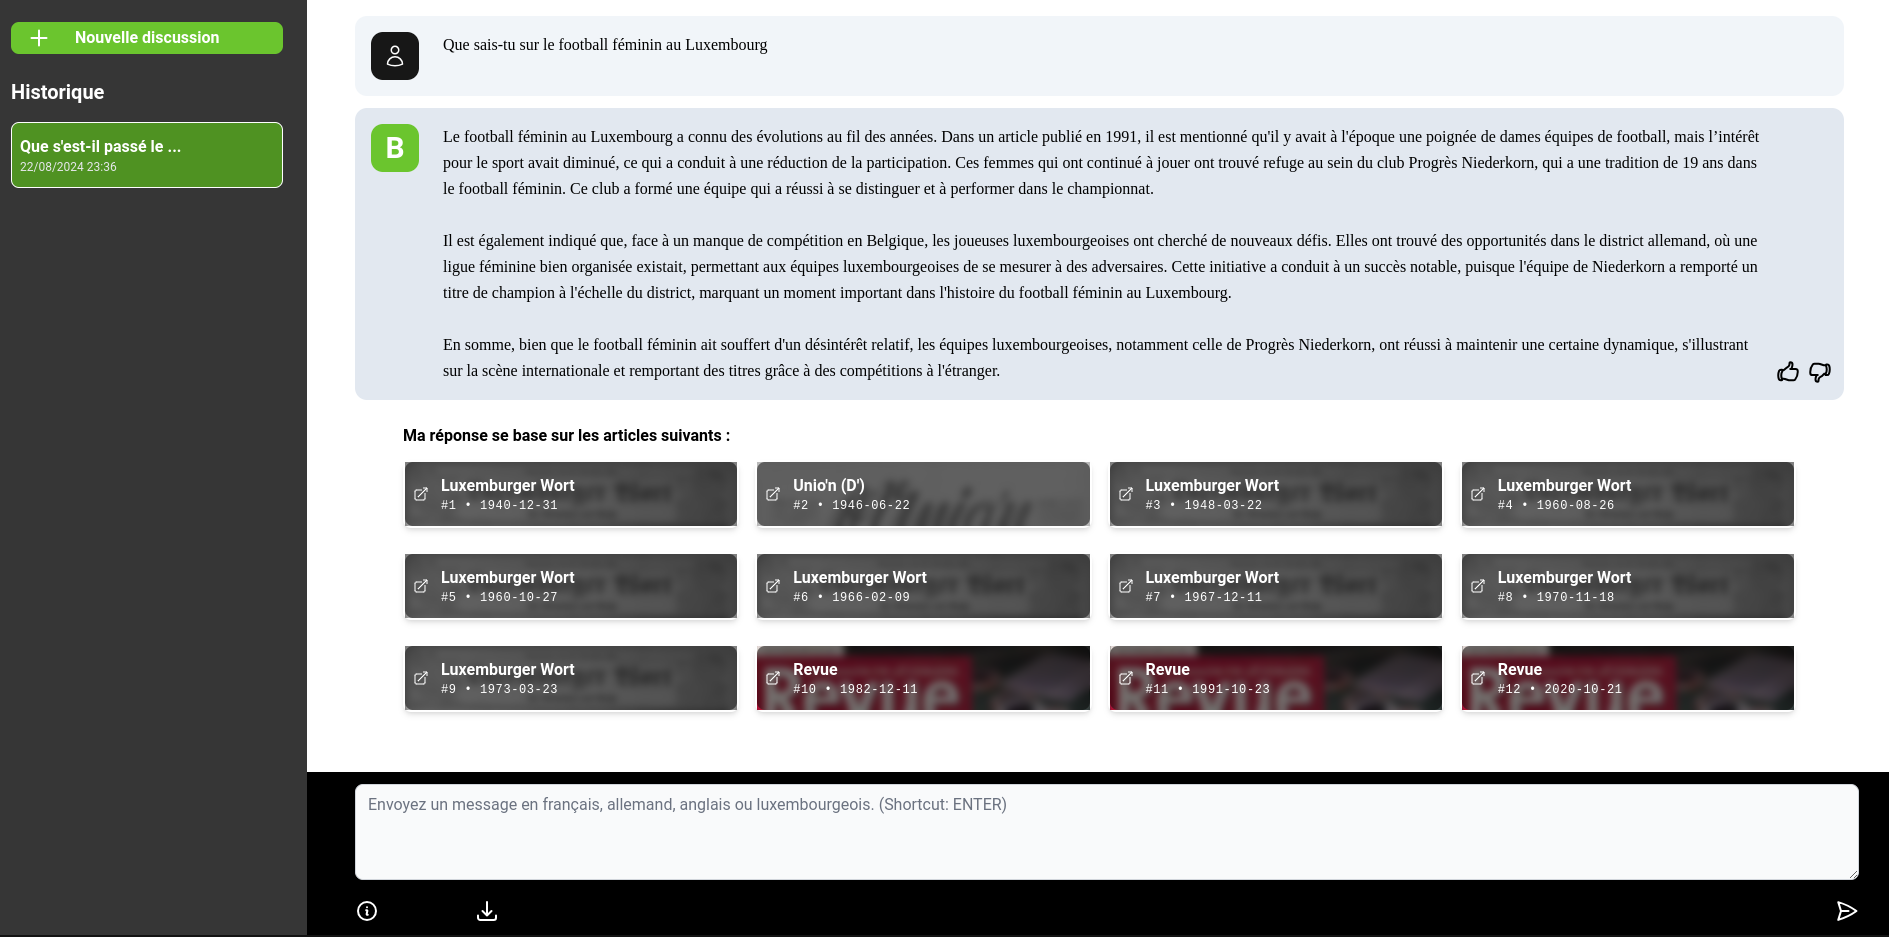
\includegraphics[width=\textwidth]{./media/image5.png}}
		\caption{Capture d'écran de l'interface du chatbot de la BNL \emph{eLuxemburgensia} }
	\end{figure}

		
		Le \emph{RAG} est une perspective intéressante en ce qui concerne la médiation dans le domaine des
	archives. Ce type d'agents joue
	un rôle dans le développement d'une forme de transparence des
	administrations avec le public mais ne remplace pour l'instant pas la
	description et l'indexation dans un moteur de recherche. Néanmoins, ces
	initiatives contribuent à procurer une visibilité plus accrue aux
	services d\textquotesingle archives, les éloignant de
	l\textquotesingle image stéréotypée de lieux poussiéreux, sombres et peu
	accessibles. Elles les présentent comme des lieux modernes et innovants.
	Elles montrent que les archives sont ouvertes à tous et à toutes, y compris au grand
	public, et pas seulement aux chercheurs ou aux passionnés de généalogie.
	Cette amélioration de l\textquotesingle image des services et cette
	démarche de médiation peuvent servir à mieux faire saisir
	l\textquotesingle importance des archives, tant au public qu'aux
	administrations dans leur ensemble et à encourager les
	investissements.\newline
	
	Les usages des grands modèles de langage et en particulier de
	l'intelligence générative conversationnelle sont donc divers dans les
	archives. Il est plus aisé de mettre en place ces technologies
	lorsqu'elles ont un faible impact en cas d'erreur. Il y a pour l'instant
	peu de recul sur ces dernières. Les \emph{LLM} ont l'inconvénient d'être
	très généraux, nécessitant d'ajuster les prompt avec des informations
	précises, des sources ou de les affiner sur des données spécifiques au
	domaine archivistique. Leur implémentation demande des connaissances
	techniques et des investissements matériels. Les recherches à venir les
	rendront peut-être plus performants sur des tâches archivistiques
	complexes ou plus légers. L'IA a un grand potentiel dans les archives
	mais nous en sommes encore au début de ses applications dans le domaine.
	Même si les projets ne conduisent pas encore à l'automatisation de
	processus complexes, ils peuvent avoir des apports connexes divers.
	
	
		\chapter{Au-delà de l'automatisation, des apports connexes~: exploration des données, collaboration et visibilité}

\subsection{La quête des données d'entraînement : exploration en profondeur des données et découverte de silos à décloisonner}


	Dans la première partie du projet InventAIre, avant de choisir une
approche et de réaliser les premier tests de \emph{machine learning},
nous avons dû regrouper des données d'entraînement et de tests. Nous
avons déjà abordé le fonds bureautique du Service des relations
européennes et internationales et du protocole (SREIP) qui a été mis à
disposition. Nous avons tenté d'obtenir d'autres documents auprès du
service Technologies de l'information, qui nous a alors présenté les bases
de données de plusieurs applications. Nous avons obtenu les fichiers pdf
des documents publiés sur le site web de la Chambre\footnote{URL~: \url{https://www.chd.lu/fr/searchactivities}}.
Il s'agit de documents parlementaires publics tels que des projets de
lois, des questions parlementaires\footnote{Questions posées par les députés aux membres du gouvernement sur l'actualité politique ou bien d'intérêt général.}, les réponses à ces
questions, des procès-verbaux publics de réunions, etc. Une extraction
de la base de données du Courrier électronique de la Chambre, dont les
documents contenant des données confidentielles ont été exclus, nous a
aussi été fournie au format csv. Le Courrier électronique est un système
d'expéditions numériques interne pour le personnel et les députés. Les
expéditions contiennent des pièces-jointes stockées dans un système de fichiers et leurs métadonnées sont stockées dans une base de
données. Les pièces-jointes peuvent être des convocations, des invitations ou encore des
projets de loi. Ce sont ces documents qui ont été mis à disposition
avec certaines de leurs métadonnées. Nous avons donc eu un aperçu d'une
partie des données stockées sur les serveurs de la Chambre et de leur
organisation. Cet aperçu nous a été révélateur de l'existence d'un grand
nombre d'applications métier différentes et de silos de données.

Les silos de données sont des systèmes de gestion de
l\textquotesingle information isolés, où les données sont stockées de
manière indépendante sans communication fluide avec
d\textquotesingle autres systèmes ou applications au sein d'une même
organisation. Les inconvénients de ces silos auraient été mis en avant à
partir des années 1980 quand a commencé à se poser la question de la
collaboration entre les services\footcite{bygstad_it_2015}. Ils peuvent en effet compliquer les projets impliquant
différentes équipes qui ne travaillent pas avec les mêmes applications
et n'ont pas accès aux mêmes données. Pour les mêmes raisons, ils
peuvent néanmoins parfois constituer une forme de sécurité. Les données
sensibles de chaque équipe restent dans les mains de ces dernières ou dans celles de l'équipe qui gère les systèmes d'informations. La
question de rassembler ces données est source d'inquiétude dans un
contexte national où, comme évoqué précédemment (chapitre 2), les
préoccupations sur la divulgation de données sensibles sont importantes.
À la Chambre des Députés, l'affaire des \enquote{\emph{ChamberLeaks}} a contribué à accroître ces dernières. Il s'agit d'une faille de sécurité qui avait permis la consultation de documents internes via de simples URL en 2018. Toutefois, les archivistes devraient idéalement pouvoir archiver les
différentes données produites par les services lorsqu'elles ont une
valeur archivistique. Par exemple, à la Chambre des Députés, le contenu
du Courrier électronique peut avoir un intérêt
patrimonial, voire juridique. Des documents officiels transitent entre
le personnel de l'administration parlementaire et les députés par cette
voie. Or, son contenu est stocké dans une base de données complexe à
appréhender et les archivistes n'y ont pas accès. Les archivistes de la
Chambre n'ont pas de vue d'ensemble des différents silos et c'est également
rarement le cas dans les autres administrations. Iels ont accès aux
applications et aux données produites par leur service. En général, ce
ne sont que quelques personnes qui travaillent côté systèmes d'information
qui y ont accès et en ont une vision globale. Par ailleurs, ces silos
peuvent causer une réplication des données, ce qui augmente par la suite le
risque de désynchronisation des informations entre les différents
systèmes. Cette réplication engendre une augmentation des besoins de
stockage. La diversité des technologies et des bases de données
utilisées complique leur maintenance, rendant les processus de gestion
plus complexes et coûteux. Enfin, avant la création
d\textquotesingle une nouvelle application, il est souvent nécessaire de
recommencer l\textquotesingle étape de modélisation des données, ce qui
ralentit les projets et génère des redondances inutiles. Le
décloisonnement des silos peut donc permettre des gains financiers.
D'après Gauthier Poupeau à propos des silos qui existaient dans les
données de l'INA, «~maintenir un système et maîtriser les données est
plus difficile et plus coûteux lorsque les silos se multiplient les uns
à côté des autres, car une telle architecture dilue les
moyens\footcite{poupeau__2024}~».

A la Chambre des Députés du Grand-Duché, il existerait entre dix et
quinze silos\footnote{Le contenu de ce paragraphe est basé sur un
	entretien avec un membre du service Technologies de l'information en
	charge du projet de refonte du système d'information de la Chambre
	des Députés.}. Ils sont à la fois applicatifs et organisationnels. En
effet, chaque service a ses applications. Il en existe par exemple une
pour gérer les procès-verbaux de commission, une pour les travaux en
commission, une pour les motions, etc. Ils sont organisationnels car
chaque application répond à un besoin métier d'un service et applicatifs
parce qu'ils sont liées à une seule application. Chaque application est
basée sur des technologies propres et a sa base de données. Il y a donc
plus d'une dizaine de bases de données différentes. Il existe toutefois
une base de données métier sous la forme d'un grand référentiel qui est
connectée aux différentes applications. Elle contient par exemple un
référentiel personne, des moyens de contact, l'organigramme de la
Chambre, etc. Cette base de données connectée évite ainsi certaines
réplications de données, mais constitue aussi une application en elle-même. Face à ces silos, plusieurs solutions existent.
À la Chambre, l'utilisation de référentiels  communs à différentes applications
est une première étape afin de créer des connexions entre silos au sein
du système d'information. Un projet de \emph{data warehouse} est
également en cours. Un \emph{data warehouse} est un regroupement de
données structurées provenant de différentes sources dans le but de
faciliter leur analyse et la prise de décision au sein d'une
administration\footcite{noauthor_quest-ce_nodate},
dans un souci d'amélioration de la \emph{business
	intelligence}\footnote{Ensemble des technologies, outils et pratiques permettant de collecter, analyser et transformer des données brutes en informations pertinentes pour prendre des décisions éclairées en entreprise.}. Le projet de la Chambre des
Députés vise à répliquer les données de chaque application en
mutualisant les différentes bases de données. Ce projet a trois
objectifs principaux. La mutualisation des bases devrait faciliter le
travail de \textit{reporting}, c'est à dire de production de rapports afin de
monitorer la qualité des données. En effet, le \emph{data warehouse} devrait
permettre de réaliser différentes datavisualisations via le logiciel
d'analyses et visualisation de données \emph{Power BI} avec des modèles
de données simplifiés. Le deuxième objectif est d'octroyer aux
différents services un moyen de visualisation de leurs données,
toujours via \emph{Power BI}. Enfin, ces données réorganisées pourront
être connectées sur la plateforme d'\emph{open data} de l'État
luxembourgeois\footnote{Plateforme \url{data.public.lu}. URL des jeux de
	données publiés par la Chambre des Députés~:
	\url{https://data.public.lu/fr/organizations/chambre-des-deputes-du-grand-duche-de-luxembourg/}}
de manière automatique afin d'être publiées et téléchargeables par
l'ensemble des citoyens. Les \emph{data warehouses} et les projets de
décloisonnement des silos en général offrent ainsi des avantages
considérables pour l\textquotesingle open data et
l\textquotesingle intelligence artificielle. En centralisant et en
structurant les données, ils permettent une meilleure accessibilité et
transparence des informations pour le public. Ils permettent également
une meilleure disponibilité de jeux de données de qualité pour
l'entraînement et les tests de modèles d'IA. Ils apportent des gains de
temps sur cette première phase de collecte et préparation de données.
L'analyse facilitée par le \emph{data warehouse} garantit aussi une
meilleure qualité des données pour entraîner des modèles.

Un second projet est en marche à la Chambre de Députés. Il s'agit d'un
projet de refonte des systèmes d'information. Cette refonte a
pour but de regrouper les différentes applications métier en une seule.
L'inconvénient d'une refonte des systèmes face au problème des silos
est son coût et le temps qu'elle demande. Dans d\textquotesingle autres
administrations publiques, la refonte peut être simplifiée par un nombre
plus réduit d\textquotesingle applications et de données à restructurer.
Cette refonte est par ailleurs une occasion de mieux organiser le
\emph{records management} au sein de l'administration. À la Chambre des
Députés, le projet a donné lieu à l'identification de quatre types
principaux de données stockées dans les systèmes. Il s'agit des données
sur les acteurs, des dossiers traités, des documents de ces dossiers, et
des regroupements de personnes (réunions, évènements). Des dossiers sont effectivement traités
par des ensembles d'acteurs, qui produisent différents documents pendant
ce processus de traitement. Les documents, et idéalement l'ensemble des
données ayant une valeur archivistique devraient être conservées. Le
projet de refonte donne un regard sur ces données à archiver et fait
émerger des réflexions quand à leur archivage. Aux archives municipales
de la ville d'Amsterdam, une refonte du système informatique a
récemment été l'occasion de réfléchir à une meilleure gestion et
conservation des archives numériques. L'équipe a développé une
intégration des fonctions d'archivistiques dès la création du système
d'information\footcite{cristia_information_2020}.
Il s'agit de la méthode nommée \emph{archiving-by-design}. Cette
refonte a également permis de revoir les formats de métadonnées afin
de faciliter l'adoption du modèle de description archivistique
RiC-O\footcite{noauthor_ric_nodate}. La reprise des systèmes
d'information face au problème des silos est donc une opportunité
d'optimiser les pratiques d'archivage et de \emph{records management}.

Il existe d'autres manières de décloisonner les silos. Un deuxième
exemple est celui de l'INA (Institut national de
l\textquotesingle audiovisuel) en France. Un «~lac de données~» a été
développé dans un souci de «~recentralisation des systèmes d'information
constitués en silos\footcite{poupeau__2024}~».
Il s'agit d'un système de stockage de données brutes et hétérogènes
provenant de diverses sources au sein du système d'information. Plusieurs projets IA ont été menés à l'INA. Le décloisonnement des silos
grâce au lac de données y est également un moyen d'avoir accès à des
données propres et centralisées et à des systèmes performants pour
faciliter les automatisations via l'IA~: «~disposer d'une
infrastructure centralisée pour toutes les données de l'INA {[}lui{]}
ouvre également une nouvelle perspective : celle de pouvoir automatiser,
en s'appuyant sur des technologies d'intelligence artificielle, la
production d'un certain nombre de données\footcite{poupeau__2024}~».
La question des silos s'est aussi beaucoup posée en bibliothèque. Nous avons trouvé moins de littérature
l'abordant du point de vue des archives.
\newline

Pour conclure sur ces problématiques de silos et de
décloisonnement, la phase de collecte et de préparation des données des
projets IA donne lieu à une exploration des données présentes dans les
systèmes de l'administration qui les initie. Cette exploration peut mettre
en évidence les failles de leur organisation. Elle a ainsi des apports
pour les personnes gérant les systèmes d'information. La collaboration
avec les services gérant ces derniers dans les administrations
paraît également inévitable pour l'archivage d'une grande partie des
données qu'ils produisent. La recherche de données pour notre projet IA
a révélé une partie de la face cachée de cet iceberg des données
cloisonnées des systèmes d'information. Au delà des apports en termes
d'automatisations, les projets IA ont aussi des apports d'ordre
stratégique. Le décloisonnement des silos identifiés offre quant à lui
une opportunité de produire des données de meilleure qualité et mieux
extractibles pour entraîner ou tester des modèles de \emph{machine
	learning}. Si les archivistes sont inclus dans le processus, cela peut
avoir un impact positif sur la gestion des archives produites par les
systèmes. La découverte des silos fait aussi ressortir le silo dans
lequel se trouvent souvent les archivistes. Cantonnés à des rôles trop
précis, ils n'ont parfois pas une vision globale sur les systèmes
d'information. En effet, les archivistes ont souvent été présentés comme
des «~généralistes de l'information\footcite{banat-berger__2012}~».
D'après Françoise Banat-Berger dans un article publié en 2012 dans la
Gazette des archives intitulé «~"Un métier à part entière, l'archiviste
un généraliste de l'information" : qu'en est-il en 2012 dans le nouvel
environnement numérique ?~» , 

\begin{quote}
L'archiviste est un professionnel bien
singulier aux confins de la science de l'information, de
l'archivistique, du juridique, de la qualité, des sciences
administratives et historiques\footcite{banat-berger__2012}.
\end{quote}
\begin{quote}
	La phrase de Gérard Naud : "un métier à part entière, l'archiviste un
	généraliste de l'information" ou, comme l'écrit aujourd'hui Jean-Michel
	Salaün un "architecte de l'information", reste par conséquent tout à
	fait opérante avec une nécessité de travailler avec un périmètre de plus
	en plus large de partenaires\footcite{banat-berger__2012}.
\end{quote}

Les projets IA appliqués aux archives numériques soulignent
l\textquotesingle importance de ce rôle généraliste des archivistes,
mettant en évidence la nécessité de collaborer étroitement avec divers
acteurs, dont les informaticiens et responsables de projets numériques, pour optimiser la gestion des
documents et l'automatisation des processus archivistiques.

\subsection{Des apports moins techniques : des projets qui renforcent les liens entre les services et apportent une visibilité sur le monde des archives}

La visibilité du monde des archives et sa collaboration avec d'autres
domaines est importante pour plusieurs raisons. La question de la
collaboration est abordée dans le code de déontologie de l'\emph{ICA (International Council on Archives)}. Le dixième article stipule
que~:

\begin{quote}
	Les archivistes travaillent en collaboration avec leurs collègues et
	les membres des professions voisines afin d\textquotesingle assurer
	universellement la conservation et l\textquotesingle exploitation du
	patrimoine documentaire. Les archivistes cherchent à stimuler la
	collaboration et à éviter les conflits avec leurs collègues, en
	résolvant les difficultés par l\textquotesingle encouragement à
	respecter les normes archivistiques et l\textquotesingle éthique
	professionnelle. Les archivistes coopèrent avec les représentants des
	professions parallèles dans un esprit de respect et de compréhension
	mutuelle\footcite{noauthor_code_nodate}.
\end{quote}

La collaboration est donc une valeur fondamentale dans le domaine
archivistique. D'après Sylvie Forastier dans un article publié dans la
\emph{Gazette des archives} sur son expérience de \emph{records manager} pour un
cabinet d'avocat international au Luxembourg, «~il serait réducteur
d'envisager un service d'archives comme étant uniquement à vocation
administrative interne, un service d'archives n'est pas totalement
déconnecté du monde externe et des activités générales de
l'entreprise\footcite{forastier_archiviste_2015}~» et il « ne fonctionne pas en autarcie
mais participe à la dynamique de l'entreprise\footcite{forastier_archiviste_2015}~». Se faire connaître auprès des autres services est
effectivement essentiel pour que les données et documents à archiver de
chacun d'entre eux soient mis à disposition. Une bonne compréhension du
fonctionnement des ces services est obtenue après des discussions avec
leur personnel et permet de mieux connaître les documents produits et
leur contexte. L'archiviste est alors au fait des différents processus
de travail et peut adapter la stratégie d'archivage. Avec l'émergence
des documents numériques, l'archivistique n\textquotesingle est
aujourd'hui plus limitée aux trois âges théorisés d'Yves
Pérotin\footnote{Yves Pérotin, \enquote{L\textquotesingle administration et les \enquote{trois âges} des archives}, \emph{Seine et Paris}, 20, (octobre 1961), p. 31-33}, mais il s'agit d'une «~archivistique des flux~»\footcite{guyon_archivistique_2022}. Les archivistes doivent idéalement être impliqués dès
la création des documents numériques, «~dès l'âge courant, c'est-à-dire
dès la conception des systèmes d'information\footcite{guyon_archivistique_2022}~». Comme évoqué précédemment, les
archivistes sont désormais des «~généralistes de
l'information\footcite{banat-berger__2012}~» et ils traitent tout type
de données. Or, d'après Jenny Bunn, \emph{Head of Archives Research} aux
Archives nationales britanniques, la tendance serait à une
spécialisation du personnel, qui peut générer des silos\footcite{jaillant_are_2024}. Les administrations et les archives pourraient donc tirer
parti de collaborations interdisciplinaires plus récurrentes\footcite{jaillant_are_2024}.\newline

Par ailleurs, pour mener à bien des projets
d\textquotesingle intelligence artificielle, une collaboration étroite
avec les acteurs informatiques et les responsables de la sécurité des
systèmes d'information (RSSI) est indispensable. Les projets peuvent exploiter
l\textquotesingle expertise des chefs de projets informatiques, de
développeurs et autres professionnels de l'informatique, qui sont par la même occasion
 sensibilisés aux enjeux archivistiques, en général assez flous
pour eux. Ils peuvent alors prendre plus naturellement en compte
les préoccupations archivistiques au moment du développement informatique.
La collaboration entre archivistes et informaticiens, bien que
stimulante, est complexe, car elle nécessite une compréhension mutuelle
entre deux mondes parfois perçus comme très différents, les archives
étant parfois considérées comme une préoccupation supplémentaire non
primordiale pour les personnes issues du monde de l'informatique. La
communication peut également être délicate à mettre en place. Cette idée
est évoquée dans un article datant de 2021 intitulé «~How AI Developers
Overcome Communication Challenges in a Multidisciplinary Team: A Case
Study\footcite{piorkowski_how_2021}~». Les
équipes n'ont pas les mêmes connaissances et les personnes qui ne
maîtrisent pas l'informatique peuvent avoir de trop hautes attentes. Il
est donc important de travailler avec des personnes capables de faire le
lien entre les acteurs, qui maîtrisent à la fois le langage du monde de
l'informatique et des sciences de l'information. Des collaborations
récurrentes pourront mener à une meilleure littératie numérique chez les
archivistes et une compréhension plus approfondie des besoins de chaque
partie prenante.

Une collaboration avec d\textquotesingle autres services est également
envisageable pour obtenir les données d\textquotesingle entraînement
nécessaires. Cette collaboration renforce alors les liens en impliquant
les services qui fournissent eux-mêmes leurs données, devenant ainsi
proactifs dans le travail archivistique. Dans le cadre du projet
InventAIre, nous avons eu des liens avec les services RH et des
relations européennes, internationales et du protocole. Ils ont dès
lors été mis au courant de l'existence de notre projet. Les projets
d\textquotesingle IA apportent en effet également une certaine publicité
aux archives, même s'il convient de rester vigilant face aux risques de
mauvaise publicité en cas d'échec. Ils démontrent que le domaine
peut aussi pousser l'innovation et est utile. Nous avons par ailleurs
tenté une collaboration avec les Archives nationales du Luxembourg pour
obtenir des données de test. La collaboration peut s'étendre au-delà
d'une administration et favoriser les synergies entre administrations.
\newline 

Les contributions des projets d\textquotesingle intelligence
artificielle dans le domaine des archives vont bien au-delà de simples
automatisations. En effet, l\textquotesingle interaction avec le
personnel d\textquotesingle autres services et
l\textquotesingle exploration de leurs données peuvent être profitables
pour toutes les parties impliquées. Ces projets IA offrent par
conséquent des bénéfices variés dans des secteurs tout aussi variés.	
		\chapter{Ce que les archives peuvent apporter à l'IA}

\subsection{Maîtrise des normes, données structurées et	classées}

	
	L'IA a beaucoup à apporter aux archives et aux autres domaines dans les
	administrations, mais le monde des archives a également beaucoup à
	apporter à l'IA. Comme évoqué précédemment, des données bien structurées
	dans un système d'information efficace sont un atout pour le
	développement de modèles de \emph{machine learning}. De par les grandes
	quantités de documents conservés par les services d'archives et leurs
	habitudes de structuration de ces données, les relations peuvent être
	bilatérales entre IA et archives. Non seulement l'intelligence
	artificielle offre la possibilité d'automatiser des traitements
	archivistiques, mais le monde des archives peut aussi être un fournisseur
	privilégié de données d'entraînement structurées. Tout d'abord, les
	données sont disponibles en grandes quantités. Le site internet des Archives
	nationales du Luxembourg mentionne quarante-cinq kilomètres linéaires de documents
	d'archives papier et vingt-cinq mille microfilms répartis entre onze groupes de
	fonds décrits\footnote{ANLux, \enquote{Fonds et collections},
		\textsc{URL}~: \url{https://anlux.public.lu/fr/rechercher/fonds-collections.html}}.
	Il n'y a pas d'information sur les archives nativement numériques. En
	France, aux Archives nationales, «~253 applications informatiques, 94
	114 910 fichiers de bureautique générés par des traitements de texte, 94
	382 photos numériques ou enregistrements sonores et audio numériques~»
	auraient été collectés entre 1983 et 2015\footnote{FranceArchives, \enquote{Panorama des archives électroniques conservées aux Archives nationales}, 
		\textsc{URL}~: \url{https://francearchives.gouv.fr/findingaid/b4bac9c0ed8ffa3f2451fbe6f6cb4c65f5a4e753/}}.
	Le site internet des Archives nationales américaines mentionne quant à
	lui plus de trente-trois milliards de documents d'archives électroniques, soit 
	huit cent trente-sept
	tera\footnote{National Archives, \enquote{National Archives by the numbers}, \textsc{URL}~: \url{https://www.archives.gov/about/info/national-archives-by-the-numbers}}.\newline
	
	Les archives conservent non seulement de grandes quantités de documents classés, mais le domaine a également une longue tradition de description, d'abord sous la forme d'inventaires.
	Des normes de description archivistique ont ensuite émergé à partir des années 1980, notamment dans le monde
	anglo-saxon, sous l\textquotesingle influence des bibliothèques. En
	1989, le Conseil international des archives (\emph{ICA}) a convoqué des experts pour établir un plan
	d\textquotesingle action international sur la normalisation des
	pratiques archivistiques. Au cours des années 1990,
	l\textquotesingle intérêt pour ces normes a progressivement augmenté,
	donnant lieu à l\textquotesingle introduction d'une première norme
	internationale, l'ISAD(G), en 1993\footcite{nougaret_vers_1995}. Elle avait pour but d'améliorer
	l\textquotesingle efficacité des pratiques archivistiques, de
	professionnaliser le métier d\textquotesingle archiviste, en permettant
	notamment d'uniformiser les méthodes
	d\textquotesingle enseignement\footcite{motte_normalisation_2015}.
	L'introduction de normes visait également à offrir une présentation homogène des archives
	pour le public, à faciliter la coopération entre institutions et à
	rationaliser le travail des archivistes\footcite{motte_normalisation_2015}. Cette approche
	de rationalisation est comparée au taylorisme et au fordisme par les
	archivistes Bénédicte Grailles et Laurent Ducol dans un article publié
	dans la \emph{Gazette des archives} en 2012\footcite{grailles_enjeux_2012}.
	Par ailleurs, d'après Céline Guyon, maîtresse de conférence associée à
	l'ENSSIB, «~la pratique archivistique s'est nourrie des innovations
	technologiques qui, en retour, ont contribué à sa
	normalisation\footcite{guyon_archivistique_2022}~». Les outils informatiques de traitement auraient
	entraîné cette normalisation et une homogénéisation des
	pratiques\footcite{guyon_archivistique_2022}. Nous avons pu voir que la normalisation répond aussi à
	des problématiques d'efficacité, néanmoins, les formats numériques
	normés sont surtout nés par besoin de communication entre les systèmes. Ils ont
	permis d'accroître l'interopérabilité entre services.
	L\textquotesingle \emph{EAD} (\emph{Encoded Archival Description}) a
	été développé dès 1993 en s\textquotesingle inspirant des bibliothèques
	et de leur format MARC et a permis de répondre à des besoins de
	diffusion d'instruments de recherche sur internet\footcite{dooley_encoded_1997}.
	Depuis, d\textquotesingle autres normes sont apparues, telles que
	\emph{RiC (Records in Context)}, dont la version 1.0 a été publiée en mai 2024, ou le
	SEDA (Standard d'Échange de Données pour l'Archivage), norme
	française d'interopérabilité utilisé pour le traitement d'archives
	nativement numériques. Ces normes sont basées sur des langages de
	structuration de données spécifiques. Les plus
	récurrents sont l'XML et le JSON.
	L'EAD est par exemple un format basé sur l'XML. 
	
	L\textquotesingle interopérabilité est
	une préoccupation dans le domaine archivistique. En France, le format
	EAD est poussé par la plateforme \emph{FranceArchives} pour
	garantir cette dernière et ainsi produire un portail unique contenant
	des instruments de recherche de plus d'une centaine partenaires. Les
	Archives nationales du Luxembourg produisent également des instruments
	de recherche en EAD pour certains de leurs fonds, notamment
	numériques. Cependant, les normes n'existent pas partout. À la Chambre
	des Députés, l\textquotesingle adoption de normes est encore en
	réflexion. L\textquotesingle inventaire des Archives nationales peut
	constituer une forme de normalisation, même si un fichier Excel
	n\textquotesingle est pas très interopérable.
	
	La production de données structurées dans les archives facilite 
	l\textquotesingle entraînement et les tests de modèles
	d\textquotesingle IA. La question de l\textquotesingle entraînement des
	grands modèles de langage sur les données des bibliothèques en ligne a
	déjà été débattue, notamment autour de la problématique du droit
	d'auteur. Elle ne s\textquotesingle est pas encore posée de manière
	significative pour les archives. Néanmoins, avec les vastes quantités de
	texte disponibles dans les fonds, qu\textquotesingle ils soient
	numérisés ou nativement numériques, et la normalisation de la
	description archivistique, cette question pourrait se poser davantage à
	l\textquotesingle avenir. Il faudra déterminer dans quelle mesure il est
	souhaitable que les archives contribuent à
	l\textquotesingle entraînement des modèles d\textquotesingle IA,
	notamment ceux développés par des grandes entreprises privées hors UE. Une des
	premières questions à se poser concerne l\textquotesingle accès à ces
	données. Faut-il les intégrer dans des initiatives
	d\textquotesingle \emph{open data}, permettant ainsi un accès libre et gratuit
	pour le développement de modèles d\textquotesingle IA, ou au contraire,
	envisager une monétisation de cet accès, en négociant avec les
	entreprises souhaitant utiliser ces données pour entraîner leurs modèles
	? Cette décision aura un impact direct sur la visibilité et
	l\textquotesingle utilisation des données nationales dans des outils
	largement utilisés par le grand public. Si ces données ne sont pas
	intégrées dans les corpus d\textquotesingle entraînement des modèles les
	plus répandus, il y a un risque que le patrimoine documentaire du pays
	soit sous-représenté, voire invisible. Une ouverture totale des données
	pourrait offrir plus de visibilité sur les archives. Cependant, cela
	nécessite de faire la balance entre les enjeux économiques, culturels et
	éthiques. La protection des droits d\textquotesingle auteur, la
	confidentialité des données sensibles et l\textquotesingle équilibre
	entre partage et exploitation sont autant de facteurs à prendre en
	compte. Le monde des archives a ainsi du potentiel pour enrichir celui de
	l'intelligence artificielle grâce à ses données structurées et
	normalisées, dans un monde où l'information prend de plus en plus de
	valeur.
	

\subsection{Une certaine maîtrise de la description : l'opportunité de renforcer la transparence des données produites par les algorithmes}
	
	D'après Herbjørn Andresen, professeur d'archivistique à l'université
	d'Oslo, dans un article intitulé «~A discussion frame for explaining
	records that are based on algorithmic output~» publié en 2019, le
	contenu généré par des algorithmes est difficilement explicable. Il est
	complexe à analyser dans le cadre du \emph{records management},
	pourtant, son explicabilité est en partie une obligation
	légale\footcite{andresen_discussion_2019}. En effet, l'article 13 du
	RGPD oblige la transparence «~des informations utiles concernant la
	logique sous-jacente, ainsi que l\textquotesingle importance et les
	conséquences prévues de ce traitement pour la personne concernée~» en
	cas de prise de décision automatisée dans le traitement des données
	personnelles\footcite{noauthor_reglement_nodate}.
	Herbjørn Andresen aborde également dans son article l'émergence de la
	question de l'éthique algorithmique. Les algorithmes nécessitent des
	explications contextuelles. L'auteur propose la réalisation de
	recherches sur les concepts de description provenant du \emph{records
		management} qui resteraient applicables et ceux qui seront à
	développer\footcite{andresen_discussion_2019}. Des réflexions sont donc à mener sur la description
	archivistique des documents et données produites par des modèles
	d'intelligence artificielle.\newline
	
	Une documentation technique est en général établie lors du développement
	de systèmes informatiques. Elle sert à la correction de bugs par les
	équipes de développement, à réinstaller les applications sur d'autres machines ou
	à adapter les systèmes à de nouveaux environnements. C'est ce que nous
	avons cherché à accomplir avec la documentation de l'application codée
	dans le cadre du projet \emph{InventAIre} en produisant une
	documentation technique aussi précise que possible. Cependant, avec le
	recul, il apparaît que cette documentation aurait pu être encore plus
	détaillée, notamment pour améliorer la transparence de l'outil. Il est
	également important d'informer le lecteur ou la lectrice que les
	inventaires ont été produits par IA. Cela pourrait inclure des
	métadonnées précisant qu'ils ont été générés par une IA, des filigranes
	ou des informations intégrées directement dans les fichiers JSON et
	Excel produits. Nous aurions pu mettre à profit nos connaissances
	archivistiques et celles de notre équipe. La description archivistique
	peut en effet être complémentaire à la documentation technique pour ce
	genre de données. C'est également l'avis de Jenny Bunn, qui prône une
	collaboration entre \emph{records managers} et informaticiens afin de réfléchir
	à une \enquote{intelligence artificielle explicable}\footcite{bunn_working_2020}.
	D'après la chercheuse, des concepts se recoupent entre intelligence
	artificielle explicable et \emph{records management}, même s'ils ne sont pas définis
	exactement de la même façon. C'est le cas par exemple des concepts de la
	transparence, de la confiance et de la responsabilité\footcite{bunn_working_2020}. Un
	des objectifs des services à travers la communication des archives est
	effectivement de garantir la transparence de l'administration. Cette
	sensibilité s'étend naturellement aux données ouvertes. Par exemple, les
	Archives nationales du Luxembourg publient leurs tableaux de tri sur la
	plateforme nationale \emph{open data}, renforçant ainsi l'accès et la
	transparence des informations. La mise à disposition des corpus
	d'entraînement des modèles développés ou affinés sur ce genre de
	plateformes peut être un pas vers plus de transparence en permettant
	une meilleure compréhension de ces derniers et l'identification de leurs
	éventuelles failles. Certaines peuvent effectivement être dues à des biais dans les données.
	Cette mise à disposition nécessite néanmoins que les modèles soient
	entraînés sur des données non-confidentielles.
	
	L'article de Jenny Bunn mentionne par ailleurs que les \emph{records managers} ont
	l'habitude de décrire précisément les producteurs et les contextes de
	production\footcite{bunn_working_2020}. La théorisation du principe de producteur
	émerge en relation avec la notion de fonds au XIX\up{e} siècle avec Natalis
	de Wailly, historien et archiviste\footcite{guyon_theorie_2023}. Il
	théorise en effet le concept de fonds et définit le respect des fonds
	dans une circulaire du 24 avril 1841~: il s'agit de «~rassembler les
	documents par fonds, c\textquotesingle est-à-dire réunir tous les titres
	qui proviennent d\textquotesingle un corps, d\textquotesingle un
	établissement, d\textquotesingle une famille ou d\textquotesingle un
	individu\footnote{Michel Duchein, \enquote{Le respect des fonds en archivistique : principes théoriques et problèmes pratiques}, \emph{La Gazette des archives}, 97, (1977), p. 71-96.}~». Les archives doivent donc rester
	rassemblées par producteur. Or, dans le cas des archives numériques,
	cette notion de producteur est vouée à évoluer. Les principes
	fondamentaux de l'archivistique française tels que le respect des fonds
	et la théorie des trois âges sont à questionner\footcite{guyon_theorie_2023}. Les pratiques luxembourgeoises ont l'opportunité de se nourrir
	de ces habitudes de description au sein des modèles français, mais
	également de les questionner et de se nourrir d'autres pratiques.
	L'archivistique canadienne, à travers les réflexions de Terry Cook,
	prône par exemple l'idée que le fonds est un concept bien lié à la provenance
	des documents, mais que la provenance n'est pas seulement liée au
	producteur, d'autant plus en ce qui concerne les données numériques,
	parfois manipulées par plusieurs producteurs : la provenance est liée à un processus
	métier\footnote{Terry Cook, \enquote{Mind over Matter: Towards a New Theory of Archival Appraisal}, in Barbara L. Craig  (dir), \emph{The Archival Imagination}, 1992, p. 38-70.}. La description du processus métier est donc
	une perspective intéressante en ce qui concerne la description des
	archives numériques, des archives produites par IA et des systèmes IA
	eux-mêmes.\newline
	
	De nombreuses questions se posent et les théories archivistiques françaises sont vouées à connaître des évolutions. En ce qui
	concerne les pratiques luxembourgeoises, il y a là une opportunité de se
	nourrir de ces pratiques françaises, mais surtout de les questionner, et
	de tirer parti d\textquotesingle autres approches, notamment des
	approches anglo-saxonnes. Le monde des archives et de l'informatique
	peuvent s'apporter mutuellement. Les professionnels des archives peuvent
	apporter leur sensibilité et expertise sur les questions d'explicabilité
	et de transparence au monde de l'informatique. Il est cependant
	important de noter que les pratiques de description et de classement des
	archives numériques ne sont pas encore fixes et peu théorisées à ce
	jour. Les discussions seront davantage prolifiques quand elles l'auront été. Inversement, la meilleure compréhension des outils développés et
	les pratiques de documentation technique issues du monde de
	l\textquotesingle informatique peuvent enrichir les approches
	archivistiques. La combinaison entre procédure de documentation technique et
	méthodologie archivistique, avec par exemple une description du contexte,
	du producteur et du processus métier, est un pas vers plus de
	transparence des systèmes IA. Mettre à disposition les données utilisées
	pour l\textquotesingle entraînement et l\textquotesingle affinage des
	modèles, selon les principes de l\textquotesingle \emph{open data}, est
	également une voie à explorer, bien que cela pose des défis en ce qui
	concerne les modèles pré-entraînés et les questions de confidentialité
	des données. L\textquotesingle explicabilité de l\textquotesingle IA ne
	sera jamais parfaite en raison de la complexité inhérente à ces
	technologies mais l\textquotesingle intégration de principes
	archivistiques dans le développement et la gestion des systèmes IA
	pourrait contribuer à améliorer la transparence et la confiance.\newline
	

	Pour conclure cette deuxième partie, l'intelligence artificielle a
	beaucoup de potentiel dans le domaine des archives, tant pour
	l'automatisation de processus que pour la recherche et la médiation avec
	le public. Les usages sont très divers et il est facile de s'y perdre.
	Archives et IA peuvent s'apporter mutuellement~: la technologie peut répondre à
	des besoins métier et les archives sont des sources de données
	structurées non négligeables, avec des intérêts similaires pour la
	transparence. En revanche, la complexité de mise en place d'outils
	pérennes et utiles pour les archivistes basés sur de l'IA est parfois
	sous-estimée car le potentiel séduisant de ces technologies a tendance à
	occulter les défis qu'elles impliquent.
	
	

	\part{Les défis éthiques et techniques du déploiement de systèmes basés sur l'IA}
		\chapter{Problématiques éthiques et environnementales}

	\subsection{Des risques sociaux et éthiques}

	Les risques sont loin d'être nuls en ce qui concerne les systèmes basés sur le \emph{machine learning}. 
	L'identification des risques est d\textquotesingle autant plus
	complexe que la réglementation a souvent un temps de retard par rapport
	aux avancées technologiques. À ce jour, il n\textquotesingle existe pas
	de cadre spécifique pour l\textquotesingle IA dans les
	archives. Se pose alors la question de la responsabilité en cas de
	problème : doit-elle incomber à l\textquotesingle utilisateur, au
	régulateur, au développeur, ou à la machine elle-même (si
	l\textquotesingle on considère la possibilité d\textquotesingle une
	personnalité juridique pour les systèmes d\textquotesingle IA) ? Les \gls{générative}s, en particulier, soulèvent plusieurs préoccupations. Nous
	avons déjà abordé la nature souvent opaque des systèmes
	d\textquotesingle IA, qualifiés de «~boîtes noires~», qui pose des défis
	en termes de transparence.
	
	Les phénomènes d\textquotesingle \gls{hallucination}s, c'est à dire la
	production d'informations incorrectes ou fictives par le modèle, sont
	l\textquotesingle un des principaux dangers. Rappelons ici une nouvelle fois que les
	grands modèles de langage sont des systèmes de génération de texte, et non de
	transmission d'informations factuelles. Les résultats ne sont donc pas
	toujours bons, les modèles peuvent «~halluciner~». Certains \textit{\gls{prompt}s} sont
	plus susceptibles de générer des hallucinations, tels que des \textit{prompts}
	dans une langue que le modèle maîtrise moins ou avec des fautes
	d'orthographe ou de syntaxe. Bien qu'un \emph{prompt-engineering} efficace
	puisse réduire ce risque, il ne l\textquotesingle élimine pas
	complètement.
	En outre, des informations «~périmées~» peuvent être données par les
	modèles. Afin d'éviter ce risque, ces derniers doivent être évalués et réactualisés régulièrement sur des
	données plus récentes.
	
	Loin de l'idée de neutralité parfois prônée en ce qui concerne les
	outils numériques\footcite{girard-chanudet_travail_2023}, les biais, avec les risques de
	discrimination ou de partialité constituent un danger important. Les
	systèmes de \emph{machine learning} qui ne sont pas des IA génératives
	partagent ces risques, causés en général par des biais dans les données
	d'entraînement, qui peuvent mener à des décisions injustes ou
	incorrectes. Une attention particulière doit ainsi être accordée à ces
	données en cas de développement d'un modèle maison. Un exemple de
	décision opaque et potentiellement basée sur un biais est le calcul d'un
	crédit vingt fois supérieur pour une femme par rapport à son mari par
	Apple en 2019\footcite{vigdor_apple_2019}.
	Dans le cas d'un usage en contexte archivistique, ces biais peuvent
	entraîner l'invisibilisation de certaines communautés, dont les archives
	pourraient être jugées de moindre valeur car sous-représentées dans les
	données d'entraînement, ou bien, à défaut d'être éliminées, l'indexation
	de ces archives peut s'avérer insuffisante. Cette invisibilisation de
	communautés minoritaires constitue un enjeu archivistique plus large.
	Les archives de ces dernières ont parfois été négligées ou détruites,
	contribuant à un effacement de leurs mémoires, ou leur description n'est pas assez précise,
	le vocabulaire qui leur est relatif n'étant pas inclus dans les thésaurus.
	L'un des cas les plus documentés en France est celui des archives des luttes contre le SIDA
	et des luttes LGBTQIA+. Les Archives nationales ont collecté les archives de l'association
	Act Up Paris mais de nombreuses archives d'autres associations ont été détruites\footcite{comoy_archives_2019}.
	Certains modèles d'IA semblent moins sujets aux biais que
	d'autres. Par exemple, \emph{Claude}, développé par la société
	Anthropic, a été conçu avec davantage de considérations
	éthiques.
	Ce modèle est utilisé par le Parlement européen pour son
	\emph{Archibot}. Claude est un agent \gls{multimodal} capable de traiter
	une grande quantité de texte. La version 2.1 lancée en novembre 2023
	accepte 200 000 \gls{token}\emph{s} en entrée, soit environ 150 000 mots.
	Anthropic a développé le concept d'\enquote{IA constitutionnelle}. 
	Cette dernière repose sur des principes éthiques clairs, une forme de constitution inspirée par
	des textes tels que la \emph{Déclaration universelle des droits de l'Homme}.
	Pendant deux phases d'apprentissage, le modèle évalue ses propres réponses en fonction de cette constitution et
	essaie de réduire le contenu potentiellement nocif de ses réponses\footcite{bai_constitutional_2022}.
	L'avantage de ces deux phases d'entraînement spécialisées est une perte de qualité moindre par rapport à un entraînement général pour générer du contenu inoffensif, puisque les réponses sont évaluées et modifiées une fois générées. Bien qu\textquotesingle il
	soit présenté comme plus éthique et performant, Claude n'est pas complètement exempt
	de biais ni d'hallucinations\footcite{priyanshu_ai_2024}.
	Développer des modèles véritablement impartiaux est un grand enjeu et
	revêt de grandes difficultés~: compte tenu de l'ampleur des données
	nécessaires à l'entraînement de ces modèles, elles ont de grandes
	probabilités de présenter des biais. Les biais linguistiques constituent
	une autre source de préoccupation. Les corpus d'entraînement des gros
	modèles d'IA génératives sont souvent dominés par des contenus en
	anglais, rendant ainsi d'autres langues moins visibles. Le
	luxembourgeois et les données sur le Luxembourg sont en général
	extrêmement minoritaires. À titre d'exemple, le modèle Llama 3 de meta
	est entraîné sur 95~\% de données en anglais\footcite{meta}. Cette
	domination linguistique peut rendre certains pays ou communautés, et
	ainsi cultures, invisibles dans les modèles généraux. Dès lors, les
	états peuvent être tentés de rendre leurs données facilement accessibles
	sur le web pour être visibles et prises en compte par ces modèles.
	Toutefois, il s\textquotesingle agit d\textquotesingle un choix
	stratégique et politique complexe : ils peuvent ne pas
	souhaiter contribuer à l'entraînement de gros modèles développés par de
	grandes entreprises étrangères. 
	%Citer rapport

	En outre, la génération automatique de contenu par les IA soulève des
	questions juridiques concernant le droit d'auteur et le plagiat. Les
	grand modèles d'IA générative sont entraînés sur du contenu disponible
	sur le web, qui peut par exemple contenir des données personnelles, ou
	bien des œuvres originales soumises au droit d'auteur. En effet, toutes les données qui peuvent être collectées le sont, dans l'optique d'améliorer les performances des modèles\footcite{crawford_contre-atlas_2023}. Ce contenu sensible
	pourrait ressortir au moment de l'\gls{inference}. 
	
	
	Pour atténuer ces risques, plusieurs solutions ont été proposées au fil de ce mémoire, telles
	que la documentation rigoureuse des projets,
	l\textquotesingle analyse préalable des risques, et des évaluations
	régulières des modèles pour détecter et corriger les informations
	périmées.
	
	Un dernier risque concerne les modèles hébergés dans le \emph{cloud}.
	Leur usage s'accompage d'une transmission de données à un tiers, la société 
	qui héberge le modèle. Il est donc important de veiller à éviter la transmission 
	de données confidentielles sans vérifications préalables. Si un projet IA traite des données sensibles,
	le modèles devront être installés localement dans l'administration ou chez
	 un tiers de confiance. 
	 Cette installation locale demande des moyens matériels importants et 
	 a par conséquent un impact écologique non-négligeable.
	

	\subsection{Besoins matériels et impact écologique}
		
	
	Pendant notre stage, des limitations matérielles se sont rapidement
	faites ressentir, notamment dès les premiers tests de \gls{clustering}
	lorsque nous travaillions avec un trop grand nombre de documents à la
	fois. La Chambre des Députés a dû investir dans un ordinateur et une
	carte graphique (GPU) pour que nous puissions travailler avec des
	modèles de \emph{machine learning} volumineux. Les spécifications de la machine
	achetée sont les suivantes~:
	\begin{quote}
		OS : Windows\newline
		RAM : 64 GB\newline
		GPU : Nvidia RTX A4000
	\end{quote}
	Avec cet ordinateur et cette carte graphique, nous étions en mesure de
	réaliser des inférences avec des moyens et grands modèles de langage.
	Pour éviter que l\textquotesingle inférence ne soit trop lente, nous
	avons appliqué une \gls{quantization} au modèle LlaMa 3. 
	C'est une technique de compression qui réduit la précision des calculs internes pour accélérer les inférences tout en maintenant des performances acceptables. L'outil développé pendant notre stage intègre une quantisation 4 bits pour les titres et les descriptions et 8 bits pour le repérage des données sensibles. La quantization 4 bits réduit la représentation numérique des poids des modèles, c'est-à-dire les paramètres internes du réseau de neurones qui sont ajustés pendant l'entraînement, à 16 niveaux distincts (2\up{4}), tandis que la quantization 8 bits utilise 256 niveaux (2\up{8}).
	%C'est à dire défnote. 
	% Stats perte de précision. 
	Nous avons observé que le temps
	d\textquotesingle inférence pour chaque \gls{prompt} était
	d\textquotesingle environ deux secondes avec une quantisation à 4 bits
	et d\textquotesingle une dizaine de secondes avec une quantisation à 8
	bits. Ces chiffres sont cependant relativement arbitraires puisqu'ils
	dépendent de facteurs très divers, notamment la longueur du prompt et de la
	réponse à produire. Un calcul plus précis du temps de traitement par
	\gls{token} aurait permis d\textquotesingle obtenir des mesures moins
	approximatives. Pour les tâches de génération de titres et descriptions, nous avons
	privilégié la quantisation à 4 bits, car la perte de précision par
	rapport à la quantisation à 8 bits était négligeable. En revanche, pour
	les prompts de repérage des données sensibles, nous avons utilisé la
	quantisation à 8 bits. Pour faire tourner des très grands modèles de
	langage à pleine puissance, un seul exemplaire de notre carte graphique
	n'aurait pas suffi, de même que pour le \gls{fine-tuning} de \gls{LLM}. Le
	développement de modèles maison peut être moins demandant en ressources
	mais l'investissement dans un GPU reste indispensable. 
	
	Cette nécessité
	de recourir à des machines puissantes rend l'impact environnemental de
	l'IA non négligeable, tant en termes de consommation
	d\textquotesingle énergie pour l\textquotesingle inférence
	qu\textquotesingle en raison de la nécessité d'investir dans des
	ordinateurs puissants. Le \emph{Contre-atlas de l'Intelligence artificielle} écrit par la chercheuse australienne Kate Crawford
	fournit un détail des enjeux écologiques de l'IA\footcite{crawford_contre-atlas_2023}.
	Les ressources nécessaires à la fabrication de matériel informatique sont
	tout d'abord très importantes. Il faut du lithium pour construire les batteries
	des ordinateurs et les batteries de secours pour l'alimentation des centres de données.
	Ce métal provient de mines situées à des endroits géographiques divers, comme le 
	Congo, la Bolivie ou la Mongolie.
	D'autres minéraux entrent dans la composition de matériel en plus du lithium.
	Dix-sept composants fossiles rares utilisés dans la production de matériel informatique
	sont en effet identifiés par Kate Crawford\footcite{crawford_contre-atlas_2023}.
	L'extraction de ces minéraux fossiles pose de nombreux problèmes éthiques.
	Au Congo par exemple, l'extraction du lithium est source de conflit.
	Des milices armées se battent pour le contrôle des mines. Les personnes chargées
	de l'extraction sont par ailleurs souvent exploitées et effectuent un travail dangereux.
	Le matériel informatique utilisé pour produire des modèles d'IA ou les faire tourner est fabriqué à partir de matériaux nombreux quoi doivent être acheminés. Leur extraction et le processus d'assemblage
	sont également sources de pollution.
	A titre d'exemple, la chaîne d'approvisionnement de l'entreprise Intel comporterait plus de onze mille fournisseurs
	dans plus de quatre-vingt-dix pays\footcite{noauthor_etude_2022}.

	
	Le développement de modèles maison plus légers a un impact écologique
	moins important que le développement de grands modèles de langage mais
	cet impact demeure. Les processus d'étiquetage des données, de
	développement et d'inférence nécessitent des ressources matérielles.
	L\textquotesingle entraînement des modèles, en particulier, requiert des
	machines qui fonctionnent pendant des heures, voire des jours. Dans le
	cas des \gls{LLM}, il se fait dans de grands \emph{datacenters} qui
	consomment beaucoup d\textquotesingle électricité et d'eau, principalement pour assurer le refroidissement des ordinateurs. 
	Les entreprises qui produisent des gros modèles ont à cœur de
	\enquote{maximiser les cycles computationnels pour améliorer la  performance}\footcite{crawford_contre-atlas_2023}, or, ces cycles consomment énormément d'énergie.
	Dans des pays comme la Chine, les \emph{datacenters} sont approvisionnés par de l'électricité majoritairement produite à partir du charbon\footcite{crawford_contre-atlas_2023}, ce qui génère beaucoup de pollution.
	
	Une des solutions envisagées pour limiter cet impact
	est l'utilisation de modèles avec le moins de paramètres possibles. De
	nombreuses entreprises travaillent actuellement à la réduction de la
	taille des grands modèles de langage, cherchant à développer des modèles
	plus compacts mais tout aussi performants. Cette approche pourrait
	réduire les coûts énergétiques et matériels, mais elle comporte aussi un
	risque d\textquotesingle effet rebond\footcite{guillory_impacts_2024} ou de paradoxe de Jevons~: 
	la facilité d\textquotesingle utilisation et la légèreté de ces
	modèles pourraient inciter davantage d\textquotesingle acteurs à les
	déployer sur leurs systèmes, entraînant une augmentation globale de la
	consommation de ressources. Bien que certains tentent de 
	mettre en avant des impacts écologiques positifs
	de l\textquotesingle IA, notamment pour la surveillance du changement
	climatique ou l\textquotesingle amélioration de
	l\textquotesingle efficacité des processus, ces avantages sont souvent
	contrebalancés par leur consommation en ressources ou des potentiels effets rebond. Lorsque des
	tâches sont optimisées, de nouvelles tâches émergent par ailleurs pour remplacer les
	précédentes. Les avantages potentiels de l\textquotesingle IA ne
	compensent pour l'instant pas son empreinte carbone, en particulier celle de l'IA générative.
	
	Face à ces enjeux éthiques et écologiques, Yannick Meneceur propose un
	ralentissement~: «~les impacts sociétaux et environnementaux majeurs de
	la transformation numérique de notre société nous imposeraient donc, de
	manière raisonnable, de commencer à ralentir au lieu de chercher à tout
	prix à accélérer\footcite{meneceur_trois_2021}~»,
	selon lui, il faudrait «~réserver le recours aux algorithmes à des
	besoins sectoriels très déterminés, avec une forte valeur ajoutée
	sociétale\footcite{meneceur_trois_2021}~».
	On peut argumenter que les archives ont une grande valeur ajoutée
	sociétale, surtout dans un monde où la gouvernance de l'information
	prend de plus en plus de place mais au Luxembourg 
	et dans bien d'autres pays, cette valeur n'est
	pas forcément reconnue. Dans le cadre d'une course à l'IA et
	d'un grand engouement, les projets se multiplient et leur objectif
	est de produire des résultats, peu importe leur forme et les cas
	d'usage. Il serait bénéfique pour les administrations de réfléchir à des
	moyens de mener ces derniers de manière responsable. Il est important de
	sensibiliser les acteurs aux impacts écologiques de l'IA et du
	numérique en général. L'organisation de \emph{cleaning days} se fait de
	plus en plus dans les archives. Une journée mondiale «~du nettoyage
	numérique~»,
	le \emph{Digital Cleanup Day}, a été créée en 2019. Lorsqu'ils sont organisés
	par les archivistes, les \emph{cleaning days} permettent une double
	sensibilisation du personnel des administrations, à la fois à
	l'archivage et à l'empreinte environnementale du numérique. La
	sensibilisation individuelle est-elle toutefois suffisante~? Est-ce
	qu'il faut attendre des innovations technologiques plus vertes et éthiques ou une régulation par
	les pouvoirs publics pour diminuer les impacts causés par l'IA et le
	numérique ? Les réponses à ces questions demanderaient bien plus de
	recherches que celles nous avons eu le temps de mener.
	
	
		\chapter{Un processus d'évaluation long et nécessitant des connaissances techniques}



\subsection{Un processus itératif complexe à mettre en place}

L'évaluation des modèles est un passage obligé dans la phase de recherche et développement de systèmes IA. Elle se fait à plusieurs étapes du projet. 
D'abord, il est nécessaire de sélectionner le modèle ou l'algorithme le plus adapté à la tâche d'automatisation à réaliser.
Ce choix doit être basé sur une série de tests comparatifs. Cette phase de test est un processus long et exigeant en ressources puisqu'il 
convient d'évaluer différentes solutions afin de voir laquelle est la plus performante. 
C'est ce que souligne Yves Maurer, responsable de la division informatique et de l'innovation numérique à la BNL, à propos du \gls{chatbot} développé par l'institution dans un entretien pour le magazine \emph{Archimag} : \enquote{Le plus chronophage a été de tester plusieurs alternatives pour chaque brique du projet : des modèles de langage ouverts, un autre créé par un groupe de recherche, celui de Meta et de Google\dots\footcite{noauthor_comment_nodate}}.

Pour effectuer ces tests, il faut avoir à disposition un corpus de test étiqueté ou bien évaluer manuellement chaque modèle. 
Les problématiques d'évaluation seront détaillées dans la sous-partie suivante. 
Avant le choix, des recherches sur les modèles ou algorithmes les plus adaptés est à réaliser. 
Il existe en effet un grand nombre de modèles sur le marché, et ce nombre devrait s'accroître encore davantage dans le futur.
Il est aisé de se perdre face au grand nombre de possibilités existantes, d'autant plus qu'il est difficile de prévoir la solution ou le modèle le plus performant sur la tâche à réaliser. 
Cela dépend des données disponibles, de leur volume, ainsi que de la nature de la tâche à accomplir. Le choix optimal peut donc sembler légèrement aléatoire, nécessitant une évaluation précise pour trouver la solution la mieux adaptée aux besoins spécifiques du projet.
Une deuxième phase de tests et d'évaluation se fait une fois la méthode choisie, centrée sur l'optimisation des paramètres du modèle. 
Un grand nombre de paramètres est en effet modifiable. 
Nous avons déjà évoqué les paramètres mathématiques et les \enquote{\gls{stop-words}} dans le cas des algorithmes de classification automatique dans le chapitre 4 du présent mémoire. 
Dans le cas des \gls{LLM}, de nombreux paramètres sont également modifiables et influent sur les performances. 
En voici une liste non exhaustive~:
\begin{itemize}
	\item \textbf{Température~:} Ce paramètre contrôle la créativité des réponses générées. Une faible température favorise les choix de mots les plus probables, tandis qu'une température élevée encourage la génération de texte plus varié et créatif, mais potentiellement moins cohérent.
	\item \textbf{\emph{Top-k}~:} Limite la sélection des mots suivants à un sous-ensemble des k mots les plus probables, réduisant ainsi la complexité et augmentant potentiellement la cohérence des réponses.
	\item \textbf{\emph{Top-p} ou \emph{Nucleus Sampling}~:} Ce paramètre permet aussi de sélectionner les mots suivants en fonction de leur probabilité, cette fois-ci non selon leur rang mais selon un niveau de probabilité cumulée minimal défini.
	\item \textbf{Pénalité de fréquence \emph{(Frequency Penalty)}~:} Une pénalité proportionnelle au nombre de fois où il a déjà été utilisé dans la réponse est appliquée au prochain \gls{token}. Elle réduit donc la probabilité de répétition des mêmes mots, augmentant ainsi la diversité des réponses.
	\item \textbf{Pénalité de présence \emph{(Presence Penalty)}~:} Une pénalité est appliquée au prochain \gls{token} s'il a déjà été utilisé dans la réponse. Elle est la même pour tous les \emph{tokens} réutilisés, peu importe le nombre de fois où ils l'ont été. Elle réduit la redondance dans les réponses tout en aidant le modèle à rester concentré sur le sujet principal, évitant ainsi les digressions.
	\item \textbf{Nombre maximal de \gls{token}s~:}  Définit la longueur maximale de la réponse à générer. Dans le cadre du projet InventAIre, par exemple, où seules des réponses booléennes ou des pourcentages de probabilité étaient nécessaires pour remplir les colonnes sur les données sensibles, nous avons limité le nombre maximal de tokens à 3 afin de n'obtenir que ces réponses. Cela permet surtout de gagner du temps et de réduire l'utilisation des ressources informatiques.
	\item \textbf{\emph{Stop Sequences}~:} Permet de définir des séquences de mots qui, une fois rencontrées, arrêtent la génération de texte, assurant ainsi un contrôle plus précis sur la sortie du modèle. Nous aurions également pu utiliser cette méthode dans le code de notre outil pour le projet InventAIre. 
	\item \textbf{\gls{quantization}~:} Technique de compression qui réduit la précision des calculs internes pour accélérer les \gls{inference}s tout en maintenant des performances acceptables. L'outil développé pendant notre stage intègre une quantisation 4 bits pour les titres et les descriptions et 8 bits pour le repérage des données sensibles. La quantisation 4 bits réduit la représentation numérique des poids des modèles, c'est-à-dire les paramètres internes du réseau de neurones qui sont ajustés pendant l'entraînement, à 16 niveaux distincts (2\up{4}), tandis que la quantisation 8 bits utilise 256 niveaux (2\up{8}).
	\end{itemize}

Après avoir ajusté ces paramètres, l'outil doit être soumis à une évaluation rigoureuse. 
Les résultats de cette évaluation détermineront les conditions d'utilisation du modèle~: 
si la précision est proche de 100\%, une vérification humaine minimale sera nécessaire, tandis qu'une précision moyenne exigera un contrôle plus strict par l'humain.

Par la suite, des évaluations régulières du modèle sont à réaliser afin de garantir sa pertinence au fil du temps. 
La réactualisation d'un modèle d'intelligence artificielle peut impliquer un ré-entraînement pour améliorer ses performances ou l'adapter à de nouvelles données. Si le modèle a été développé à partir de zéro, il peut nécessiter un ré-entraînement complet pour intégrer des améliorations ou des changements dans les données. Si le modèle a été affiné, il devra l'être de nouveau. Dans le cas des systèmes basés sur du \gls{RAG}, cette réactualisation inclut l'injection de nouvelles données dans la base de connaissance et leur \gls{vectorisation} pour enrichir le modèle avec des informations plus récentes et/ou pertinentes. Les \emph{LLM} conversationnels nécessitent également une actualisation régulière. Cela peut inclure la modification des prompts pour mieux refléter les nouvelles données ou les exigences spécifiques du projet. Il est aussi possible d'adopter une version plus récente du modèle choisi, qui peut ainsi amener à des améliorations en termes de performance et de capacité, ou bien de sélectionner un autre modèle plus récent et plus puissant, capable de mieux répondre aux besoins du moment et d'intégrer les avancées technologiques les plus récentes. Dès lors, les prompts devront être actualisés selon les exigences des modèles.
 Une longue phase de tests et éventuellement de ré-entraînement est donc aussi à prévoir pour en cas de changement de modèle. Les réflexions sur l'actualisation des outils mis en place doivent être accompagnées d'une veille sur l'actualité des méthodes et des modèles de \emph{machine learning}.
Une partie du processus est automatisable. Par exemple, si les résultats fournis par la machine sont constamment vérifiés par l'humain, des statistiques peuvent être aisément réalisées sur le nombre de données produites ayant dû être corrigées par le personnel au fil du temps. Si les réponses des modèles sont utilisés telles quelles, sans processus de vérification, il faudrait penser à mettre en place des pratiques de test par échantillonnage réguliers.

Ce processus itératif est à penser en amont. Le temps qu'il demande et son coût peuvent être sous-estimés, en particulier quand le choix technique se porte sur les \emph{LLM} conversationnels qui semblent être des outils \enquote{clé en main} alors que leur usage nécessite des compétences techniques non négligeables, en particulier sur l'automatisation de tâches complexes. 
Cette nature itérative a toutefois l'avantage de bien s'inscrire dans des pratiques de gestion de projet agiles cycliques.
Des statistiques d'évaluation et des visualisations de données les plus neutres possibles et faciles à comprendre sont
utiles pour valider les résultats à la fin des cycles et orienter les décisions tout au long du projet.
Néanmoins, dépendant de métriques élaborées, ces statistiques peuvent parfois être difficiles à établir.


\subsection{Quelles métriques d'évaluation pour des tâches liées au langage ?}

Pour que le processus d'évaluation soit précis, des métriques doivent avoir été définies en amont.
Les métriques de base en \gls{apprentissage} sont la \gls{précision} et le \gls{rappel}. La \gls{précision} est le ratio
de prédictions correctes par rapport à l'ensemble des prédictions et le
\gls{rappel} correspond au ratio de prédiction correctes par rapport à l'ensemble des
entités qui devraient être identifiées. La précision mesure donc la
capacité du modèle à éviter les faux positifs, tandis que le rappel
évalue sa capacité à identifier toutes les entités pertinentes. A partir de cette précision et ce rappel
peut être établi le \gls{F1-score}, qui calcule une moyenne entre les deux située entre 0 et 1.

Le calcul de cette précision et ce rappel sont relativement simples dans le cas d'une classification ou de réponses booléennes. 
Par exemple, concernant les colonnes sur les données sensibles de notre inventaire, la réponse est soit vraie, soit fausse.
Toutefois, en ce qui concerne de la génération de langage, cette analyse est plus subtile. Elles est donc plus complexe à automatiser.
En effet, il est plus aisé de faire tourner différents modèles ou bien le même modèle dont les paramètres ont été modifiés
sur des données préalablement étiquetées avec des \enquote{vrai} ou \enquote{faux} et de regarder le taux d'erreur.
Des métriques spécifiques d'évaluation du langage généré par comparaison avec un texte de référence existent. Ces dernières permettent d'automatiser l'évaluation et donc de lutter contre les inconvénients liés à la subjectivité humaine, même si cette dernière reste présente dans le texte de référence, rédigé par l'humain. En voici une liste non-exhaustive~:

\begin{itemize}[label=\textbullet]
	\item \textbf{\emph{WER (Word Error Rate)}}~: métrique au départ utilisée pour évaluer la précision des 
	systèmes de reconnaissance vocale. Elle mesure le pourcentage d'erreurs, telles que les substitutions, 
	les insertions et les suppressions, dans le texte transcrit par rapport au texte de référence.
	\item \textbf{Approches basées sur des modèles pré-entraînés}: mesurent la similarité entre le texte généré et le texte de référence en utilisant les
		\gls{embeddings} de modèles pré-entraînés. L'évaluation est donc basée sur une similarité sémantique et contextuelle. Un exemple de métrique basée
		sur un modèle pré-entraîné est le \emph{BERTScore}, avec le modèle \emph{BERT} de \emph{Google}.

	\item \textbf{Métriques développées pour l'évaluation de traductions} mais restant applicables à l'analyse de résumés.
			\begin{itemize}[label=\textopenbullet]
				\item \textbf{\emph{BLEU (BiLingual Evaluation Understudy)}}~: compare les n-grammes (mots ou séquences de mots) du texte généré aux n-grammes du ou de textes de référence, en utilisant une formule qui mesure une précision avec un ajustement selon la longueur des phrases.
				\item \textbf{\emph{METEOR (Metric for Evaluation of Translation with Explicit ORdering)}}~: mesure la qualité des traductions/résumés en comparant les n-grammes, en incluant leurs synonymes et la correspondance de leur radical, entre le texte généré et les textes de référence. Il s'agit d'une moyenne entre précision et rappel.	
			\end{itemize}
	
	\item \textbf{\emph{ROUGE (Recall-Oriented Understudy for Gisting Evaluation)}}~: développée pour mesurer la qualité de la génération de résumés, cette métrique mesure la similarité
	entre un résumé généré automatiquement et un ou plusieurs résumés de référence. Pour cela, les scores de précision et de rappel sont calculés
	en comparant les n-grammes présents dans le résumé généré avec ceux des résumés de référence.
	Une plus grande attention est accordée au score de rappel, qui évalue la quantité d'informations importantes des résumés de référence capturées par le résumé généré.\footcite{noauthor_large_2023}.
\end{itemize}

Les métriques sont donc très diverses et ne sont pas forcément aisées à saisir. Elles nécessitent un travail de réflexion en amont, et parfois des moyens techniques conséquents
lorsqu'elles sont basées sur des algorithmes complexes ou du \emph{machine learning}. Il est nécessaire de bien les maîtriser pour fournir une 
évaluation la plus précise possible.

Des \gls{benchmark}s 
plus généraux existent par ailleurs pour évaluer les grands modèles de langage. De nombreux sont disponibles en ligne\footnote{Voir par exemple ceux disponibles ici~: \url{https://huggingface.co/collections/open-llm-leaderboard/the-big-benchmarks-collection-64faca6335a7fc7d4ffe974a}}.
Ils permettent d'avoir une idée générale de leur qualité.
Dans le cadre de notre stage, pour choisir le modèle, nous avons expérimenté plusieurs méthodes d'évaluation.
La première consistait en un système de notation. Un système de notation a également été utilisé dans le cadre de la sélection d'une méthode
pour la réalisation du projet LlaMandement mentionné précédemment\footcite{gesnouin_llamandement_2024}. 
En ce qui concerne le projet InventAIre, le système de notation s'est rapidement avéré subjectif 
mais a permis d'éliminer les modèles les moins précis. Face à cette question de la subjectivité, les personnes chargées
de l'évaluation sur le projet LlaMandement avaient dans leur corpus des résumés rédigés par des humains.
La note moyenne octroyée à ces derniers s'est élevée à 16,5, ce qui donne plus de crédibilité à l'évaluation et donne une cible
à atteindre par l'IA\footcite{gesnouin_llamandement_2024}.
Après avoir expérimenté avec des notes, nous avons mis au point une évaluation comparative. 
Nous comparions les titres et descriptions générés par plusieurs modèles sur une
même unité de description afin d'établir un classement
\footnote{Plus d'informations sur l'évaluation dans la note méthodologique en annexe (partie 2.3.1. et annexe 4 et 5)}. 
Ce système garde une forme de subjectivité mais il est moins subjectif qu'un système de notation.
Nous avons effectué le travail à l'envers par rapport à ce qui se fait normalement en \emph{machine learning}. 
Un corpus de documents préalablement étiqueté est normalement séparé en deux parties, une pour l'entraînement, une pour la validation.
Adopter cette approche, et ainsi avoir préalablement étiqueté des données de test, aurait poussé l'équipe à réfléchir davantage en amont afin de se mettre d'accord sur le contenu des différentes colonnes.
Une forme de consensus est effectivement nécessaire pour l'étiquetage de données ou l'évaluation de performances.
Par exemple, une donnée peut être considérée comme sensible par un archiviste et non par un autre.
Sans lignes directrices précises, il peut y avoir autant d'inventaires que d'archivistes. Face à ce souci de subjectivité, nous avons 
mis en place un système d'évaluation finale en trois possibilités : \enquote{correct}, \enquote{incorrect} et \enquote{sujet à débat/insuffisant}.
À la Cour de cassation française, pour mener à bien le
 projet de pseudonymisation, une \enquote{élaboration théorique des catégories et [une] définition des types de contentieux\footcite{girard-chanudet_travail_2023}} a été réalisée par des juristes, malgré tout, l'exécution 
 des conseils donnés par les juristes est complexe dans la pratique. Certains termes peuvent appartenir à plusieurs catégories
 ou bien à aucune des catégories définies par les juristes\footcite{girard-chanudet_travail_2023}. Il y a alors un dialogue qui se crée et 
 certaines catégories sont précisées. Le fait d'étiqueter en amont est donc bénéfique pour amener la discussion et préciser les définitions
 des différentes catégories ou données à repérer, ou bien pour préciser la forme et le contenu du texte à rédiger.
 Un étiquetage des résumés et descriptions en amont aurait rendu l'exécution du projet InventAIre davantage productive.


La précision n'est pas la seule métrique à laquelle nous nous sommes intéressée dans le cadre de notre stage.
Nous avons également examiné le temps de génération, en calculant des moyennes par \gls{prompt}. Il aurait été davantage pertinent de mesurer le temps par \gls{token}
dans le prompt, puisque ces derniers peuvent être de tailles différentes selon la taille du document qu'il inclut.
Il y a une inférence par colonne de l'inventaire, et parfois plus d'une inférence par ligne dans le cas de documents longs qui, dépassant la capacité de la \gls{fenêtre} du \emph{LLM}, seraient divisés en plusieurs parties.
Ce temps s'accumule vite et la génération d'un inventaire peut prendre des jours entiers si l'on n'y fait pas attention. Nous aurions aussi pu évaluer les ressources dépensées pour chaque inférence par la machine.

Nous nous sommes enfin intéressée à l'évaluation des biais.
Cette dernière est complexe. Il existe des \gls{benchmark}\textit{s} publics pour estimer à quel point les modèles les plus utilisés
sont sujets au biais, ainsi que des \emph{datasets} publics pour tester les modèles maison ou affinés. C'est ce qui a été fait dans le cadre du projet
LlaMandement. Le modèle fine-tuné a été testé sur le jeu de données spécialisé \emph{BOLD (Bias in Open-ended Language Generation Dataset)}.
La réalisation de ce test suppose que les biais en français sont les mêmes qu'en anglais\footcite{gesnouin_llamandement_2024}, ce qui n'est pas forcément vrai.
Des métriques de mesurant les biais ont par ailleurs été calculées. Il s'agit de \emph{Regard} et \emph{Honest}. 
\emph{Regard} évalue la polarité du langage et les perceptions sociales de divers groupes démographiques 
(par exemple selon le genre, l'appartenance ethnique et l'orientation sexuelle), en identifiant les biais dans le ton 
ou avec une analyse des sentiments qui pourraient influencer la représentation de ces groupes\footcite{gesnouin_llamandement_2024}.
 \emph{Honest} mesure la fréquence des complétions de phrases offensantes dans les modèles de langage,
  en utilisant un lexique multilingue pour fournir un score de toxicité et détecter les disparités potentielles entre différents groupes démographiques\footcite{gesnouin_llamandement_2024}.
\newline

Les réflexions sur l'évaluation seront à pousser en cas de suite du projet InventAIre. 
Il s'agit d'une étape qui se répète tout au long du projet. Elle doit être ainsi optimisée, voire rationalisée, pour éviter de perdre trop de temps.
 Ces évaluations sont déterminantes dans le succès des projets et sont indispensables à la mise en production de systèmes basés sur de l'IA.


	
		\chapter{Problématiques de mise en production}


\subsection{Une \gls{chaîne} à mettre en place}

Le choix d'un algorithme ou d'un modèle pour accomplir une tâche donnée n'est que la première étape vers le développement d'une solution d'automatisation basée sur du \emph{machine learning}. 
Le modèle sélectionné traite des données en entrée et génère une sortie, qui doit ensuite être intégrée dans une \gls{chaîne} plus large. 
Ces données de sortie ne sont en effet pas directement exploitables en l'état. 
Dans cette section, nous décrivons la chaîne de traitement mise en place pour le projet InventAIre, afin de prendre du recul, en analysant ses forces et ses faiblesses.

Le schéma ci-dessous résume ce processus général de traitement mis en place, qui sera expliqué plus en détail, étape par étape.\newline
\begin{figure}[h!]
	\centerline{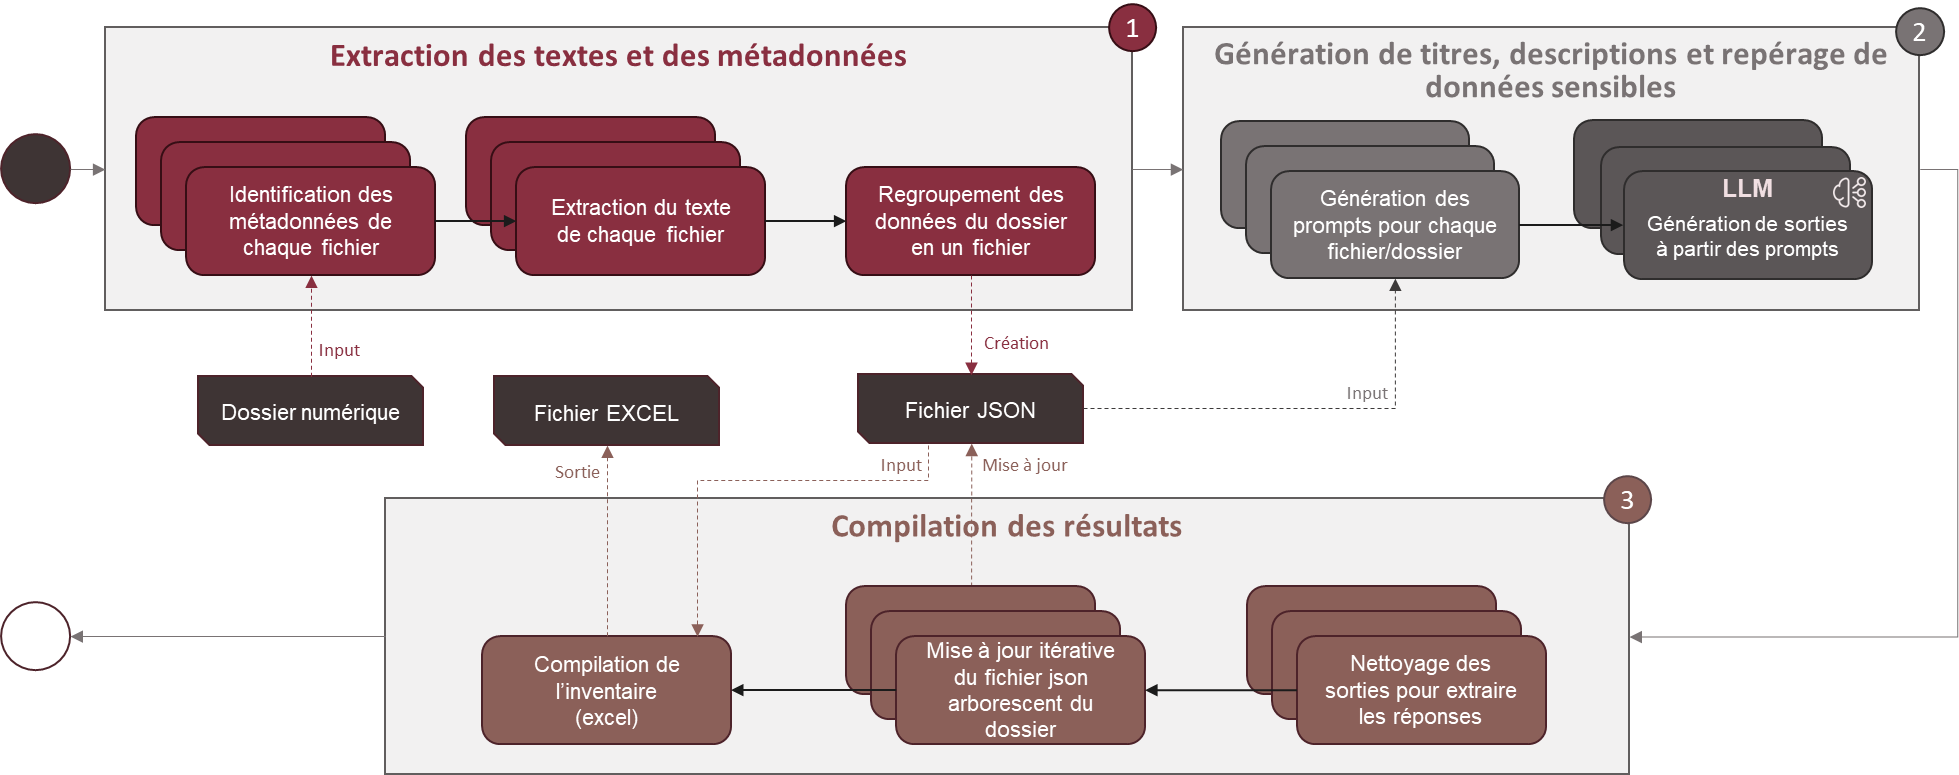
\includegraphics[width=\textwidth]{./media/process_traitement.png}}
	\caption{Processus de traitement mis en place afin de générer l'inventaire}
\end{figure}

\paragraph*{Étape 1 : Extraction des textes et des métadonnées des documents}\mbox{}\\

L'application prend en entrée un chemin de répertoire numérique.
Les métadonnées extractibles de l'intégralité du contenu de ce dernier sont compilées en un seul un fichier au format JSON, 
avec le texte de chaque document. Si le texte n'est pas disponible, une tentative d'océrisation est réalisée avec le logiciel Tesseract.
Dans le cas où les textes des fichiers seraient trop grands et dépasseraient la \gls{fenêtre} de Llama 3, ils sont divisés en différentes parties,
 que nous avons nommées \enquote{chunks}, de 10 000 caractères. Ce découpage est relativement arbitraire, nous aurions pu couper 
 au niveau de la fin d'une phrase pour que cela perturbe moins notre LLM.
 Nous aurions également pu tester avec des chevauchements entre les différents \enquote{chunks}.
 Ci-dessous se trouve un exemple de fichier JSON arborescent produit pour un dossier qui contiendrait un seul document.
 \vspace*{0.2cm}
\begin{tcolorbox}[colback=white, colbacktitle=white, coltitle=black, title=Exemple de fichier JSON arborescent pour un dossier contenant un document, center title]
  \begin{minted}[]{json}
 {
    "path": "C:\User\Chemin\du\dossier_exemple",
    "folderName": "dossier_exemple",
    "type": "directory",
    "content": [
    {
        "path": "C:\User\Chemin\du\dossier_exemple\document.txt",
        "type": "file",
        "fileName": "document.txt",
        "creationDate": "Wed May 20 10:26:26 2024",
        "modificationDate": "Wed May 29 10:35:06 2024",
        "mimeType": "text/plain; charset=UTF-16LE",
        "texte": "Ceci est le texte d'un document txt.",
        "generatedTitle": "to be defined"
    }
    ],
    "generatedTitle": "to be defined"
 }
\end{minted}
\end{tcolorbox}



\paragraph*{Étape 2 : Génération de titres, descriptions et repérage de données sensibles}\mbox{}\\

A partir du document JSON, des \gls{prompt}s sont ensuite générés pour chaque niveau dans l'arborescence et chaque donnée sensible.
Le LLM est interrogé avec ces différents prompts.
L'encadré ci-dessous en montre un exemple.
En rose se trouvent les éléments mutables selon le type d'entrée (document, dossier, chunk) 
et en vert se trouvent les éléments mutables selon la colonne à remplir.

 
\begin{tcolorbox}[colback=white, colbacktitle=white, coltitle=black, title=Exemple de prompt]

\underline{Input :}
\begin{minted}[]{json}
    {
        "path": "C:\User\Chemin\du\dossier_exemple\document.txt",
        "type": "file",
        "fileName": "document.txt",
        "creationDate": "Wed May 20 10:26:26 2024",
        "modificationDate": "Wed May 29 10:35:06 2024",
        "mimeType": "text/plain; charset=UTF-16LE",
        "texte": "Ceci est le texte d'un document txt.",
        "generatedTitle": "to be defined"
    }
\end{minted}

\underline{Context :}
You are an achivist at the Chambre des Députés of Luxembourg.

\underline{Question :}
You have been given a \textcolor{purple}{full document and some metadata} formatted as json as input. You are working on an archival inventory project.
Please generate one \textcolor{teal}{title} \textcolor{teal}{(max 20 words)} in french for this \textcolor{purple}{document} for the inventory.

\textcolor{teal}{In your title, avoid the word 'fonds'. Avoid generic words such as 'divers' or 'variés'. Also avoid the word 'documents' without further precisions : add the types or names of the documents being exhaustive (all of the major types). It would be better if you could format it this way : 'subject, topic - action/type of document', only do it if there is a clear topic or subject and a clear action or only one clear types/names of documents. If there is a chronological indication in your title (not madatory, only if you are sure and if it is pertinent, must be with the topic if it is the date of the event that constitutes the topic) the format is day (number) month (letters, no abbreviation) year (number). If there are several parts in your title, separate them with commas. Be precise and exhaustive in your title (remember : topic/subject - action(s)/precise type(s) of documents if you can) but do not put information you are not sure about. If the document's text does not give you information, do not make it up. Make sure to mention the important people, organizations, locations, dates, ... if you identify some.}

Examine well the whole content for this. Please only write the \textcolor{teal}{title} in french, nothing else, so I can directly reuse it in my inventory. 
Do not explain your answer or tell me about alternatives in your answer. I only need the \textcolor{teal}{title}. Do not invent information, only use the ones you have. 
It's ok if your answer is minimalist because you do not have enough info.
\textcolor{purple}{Be careful, sometimes a file contains several types of document.}

Make sure the syntax and spelling in french in your answer are correct.

\textcolor{teal}{title} in french :


\end{tcolorbox}

Quand le document est un dossier, c'est une arborescence plus grande qui est donnée en entrée, avec des titres et descriptions déjà générés, parce que l'ensemble des textes serait trop long et dépasserait la fenêtre du \emph{LLM}. Il en va de même pour la génération d'un titre ou d'une description pour un document composé de \enquote{chunks} : un résumé de chaque partie du document est généré
et c'est à partir de ces résumés que sont générés les descriptions et titres de ce dernier.

\paragraph*{Étape 3 : Compilation des résultats obtenus par le \emph{LLM}}\mbox{}\\

Les réponses sont extraites des résultats fournis par le \emph{LLM}~: selon le prompt, on extrait le \enquote{oui}/\enquote{yes}, le \enquote{non}/\enquote{no} ou un pourcentage de probabilité généré
 pour remplir les colonnes sur les données sensibles avec des \enquote{oui} ou des \enquote{non}.
Le fichier JSON est par la suite mis à jour de manière itérative après chaque \gls{inference} du modèle, qui correspond à un prompt.
La mise à jour du fichier JSON part du bas de l'arborescence pour remonter vers la racine. Cela permet de décrire chaque niveau en fonction de son contenu. S'il y a un grand nombre de niveaux,
 les niveaux supérieurs seront décrits en fonction du titre et de la description générés pour les dossiers et fichiers qu'ils contiennent.
 L'avantage est la description de chaque niveau. Les données sensibles repérées sont également compilées au fur et à mesure par niveau.
 Un inconvénient réside dans le fait que la description est de moins en moins précise en remontant dans l'arborescence. Les erreurs sur les données sensibles s'ajoutent également, 
 le niveau supérieur d'une grosse arborescence contient donc en général beaucoup de données sensibles alors que ce n'est pas forcément le cas.
 
 Une fois l'inférence réalisée sur l'ensemble du fichier JSON et pour toutes les colonnes de l'inventaire,
 ce dernier est compilé en un fichier Excel avec une ligne par niveau dans l'arborescence.\newline
 
 
 \begin{figure}[h!]
 	\centerline{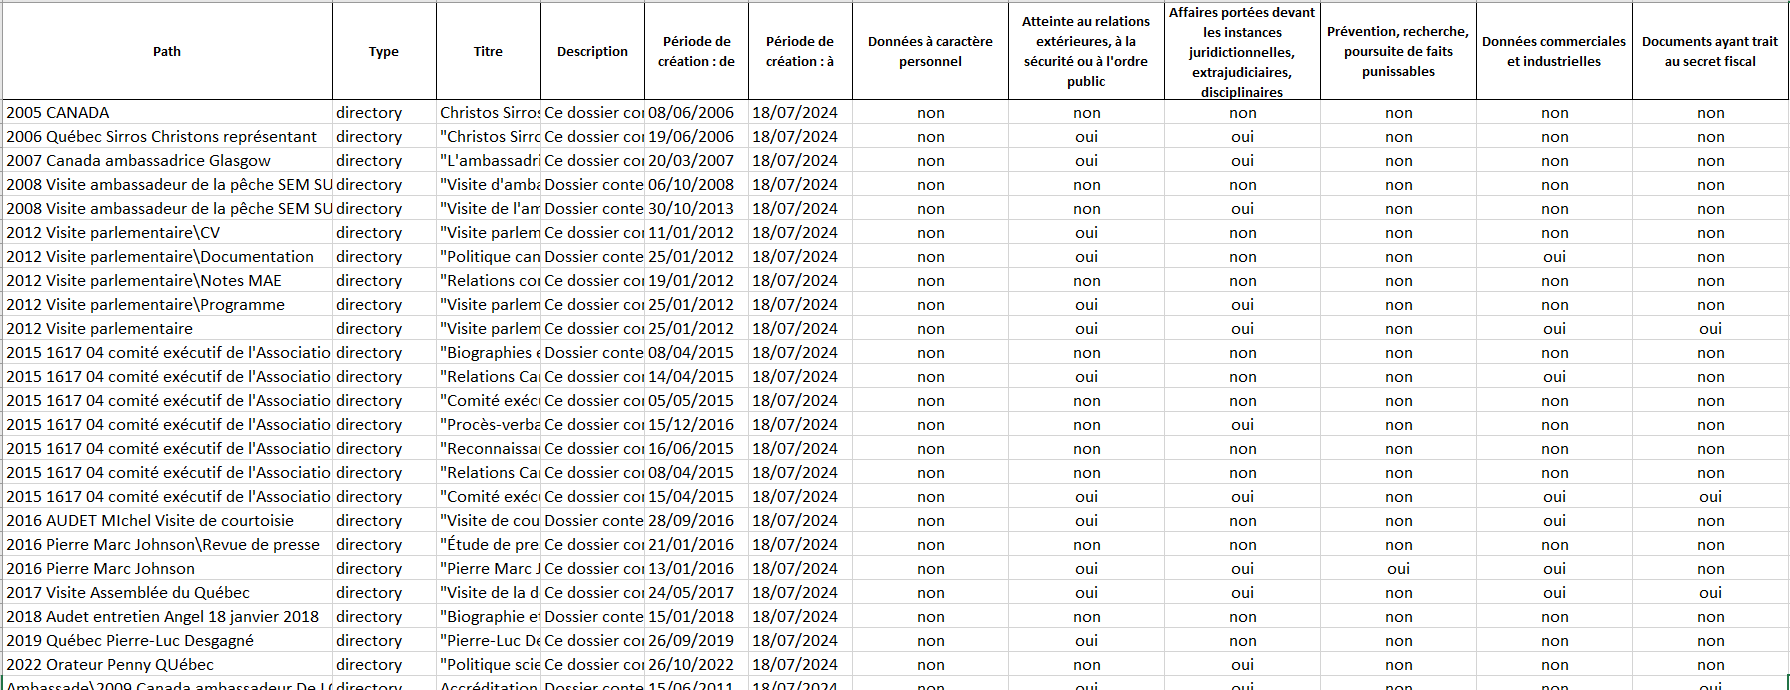
\includegraphics[width=12cm]{./media/results.png}}
 	\caption{Exemple de tableau Excel contenant les résultats d'une inférence}
 \end{figure}
 
 
\begin{figure}[h!]
	\centerline{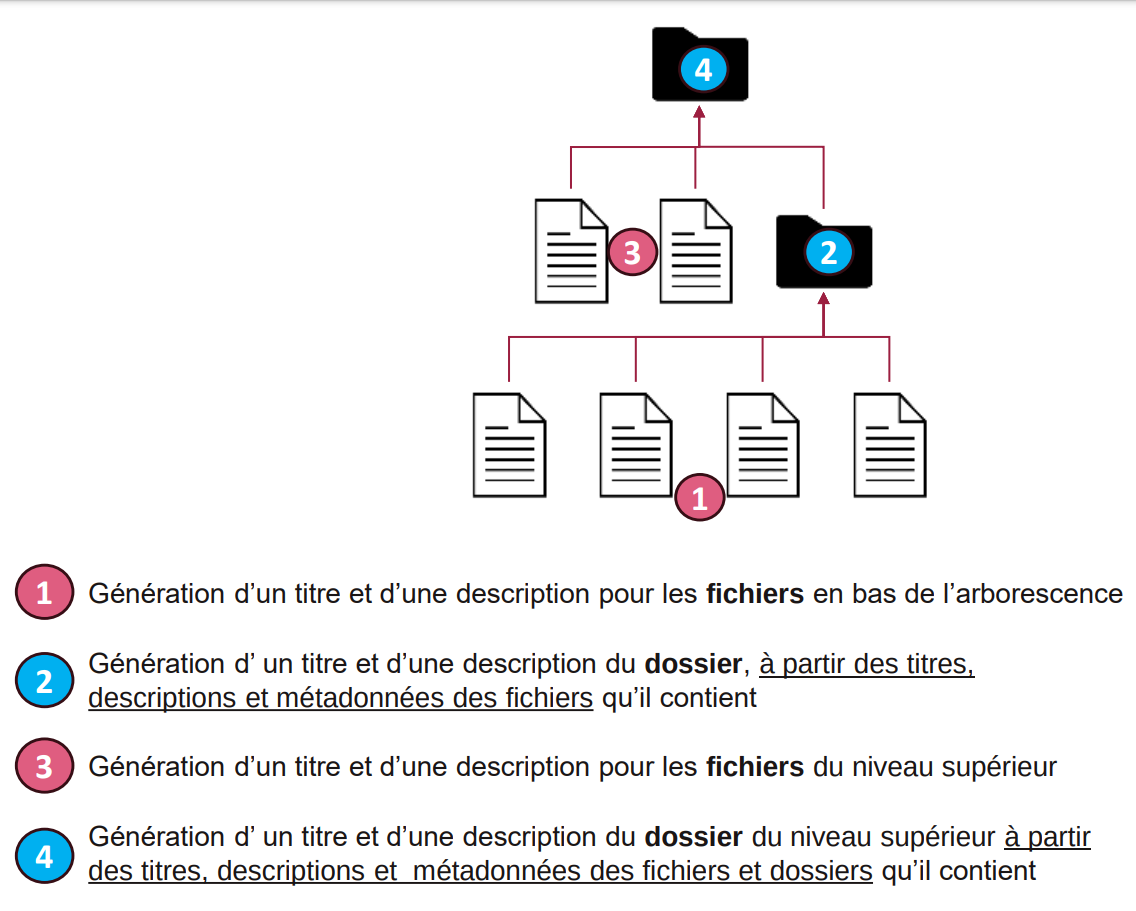
\includegraphics[width=12cm]{./media/remplissage_json.png}}
	\caption{Schéma du fonctionnement de l'inférence pour traiter chaque niveau d'arborescence dans le cas de la génération de titres et descriptions}
\end{figure}





Avec un peu de recul, nous pouvons dire que cette chaîne de traitement et le code en général sont assez complexes. Elle n'est pas composé de beaucoup d'étapes très distinctes les unes des autres, 
mais le traitement itératif pour chaque niveau de l'arborescence et chaque colonne à remplir est long, composé de beaucoup de variables et peut donc être difficile à saisir.
La mise en place d'un outil de traitement qui contient une composante IA demande des capacités techniques et peut être un réel défi intellectuel, comme cela a été le cas pendant notre stage.
Nous avons eu du mal à réaliser un outil capable de traiter tous les niveaux et la solution choisie n'est peut-être pas la meilleure.
On pourrait la qualifier de \enquote{bricolage}. Il en va de même pour les prompts. Nous avons réalisé de nombreux tests pour voir lesquels fonctionnaient le mieux. Au final, cela a produit des prompts très longs
 et peut-être trop précis parfois.

Nous avons souhaité qu'il y ait une grande granularité dans la description.
Elle comporte plusieurs niveaux 
et se répète parfois, ce qui est contraire à certaines normes de description archivistique, comme la norme ISAD(G). Ce n'est pas forcément utile, 
cela peut générer du bruit en cas de recherche ou bien générer des descriptions peu précises et ainsi inutiles.
Il y a un juste milieu à trouver entre ce qu'il est utile de décrire et ce qu'il est possible de faire grâce à l'IA. 
En France, à l'INA, un travail a été réalisé pour trouver cet équilibre. Les pratiques de description ont même évolué grâce à l'IA.
D'après Eléonore Alquier, directrice adjointe Data \& Technologies, \enquote{l'enjeu du recours à l'IA n'est plus de poursuivre à l'identique la production documentaire \enquote{classique}, mais
	de générer, de manière industrielle et sur la durée, des clés d'entrée nouvelles dans les collections, sur un mode analytique
	et synthétique\footcite{IA_INA}}.
Et si l'IA n'était pas seulement une solution d'automatisation de tâches métier mais le moyen d'ajouter autre chose, de faire évoluer les pratiques archivistiques ?

 Lorsque les tâches à réaliser demandent beaucoup de réflexion ou d'étapes, les chaînes de traitement contenues dans les outils développés s'alourdissent et
les automatisations peuvent perdre en précision.
L'IA, bien que puissante, doit être intégrée avec précaution et réflexion dans les pratiques archivistiques existantes 
 pour en maximiser l'efficacité tout en évitant les écueils liés à des tentatives d'automatisation excessives ou mal adaptées. 


\subsection{Interface et intégration à la chaîne archivistique}

Ce long processus doit par la suite s'intégrer à la chaîne archivistique. La chaîne archivistique peut se définir comme
\enquote{l’ensemble des activités de l’archiviste, depuis la collecte jusqu’à la communication éventuelle des documents, en passant par le traitement physique et intellectuel des documents\footnote{Elisabeth Bellion, \enquote{Journée d’études: Les revues et leurs archives. Méthodologie d’archivage}, carnet Hypothèses \emph{ArchiSHS}, \textsc{URL}~: \url{https://archishs.hypotheses.org/tag/chaine-archivistique}}}. 
Ces activités sont des processus en eux-mêmes et peuvent être traités à l'aide de différents outils. 
Par exemple, il existe des logiciels de gestion et de description des archives. 

%%%%ici
Les systèmes IA développés doivent pouvoir être facilement utilisables par les équipes afin de s'intégrer
efficacement à cette chaîne. Pour cela, la production d'un logiciel avec une interface est indispensable : tous les archivistes ne maîtrisent pas les outils qui fonctionnent en ligne de commande. Ce dernier ne doit pas non plus exiger une formation trop longue. Il doit être intuitif et engageant. Un exemple d'interface de système basé sur le \emph{machine learning} qui pourrait être améliorée est celle de Pêle-mél.
Bien que fournissant des visualisations utiles sur les contenus des boîtes mail, elle peut être jugée comme trop complexe, 
ce qui peut freiner l'adoption d'un outil malgré sa qualité. Toutefois, elle a l'avantage de contenir beaucoup de moyens de personnalisation.
Le bilan du projet mentionne que \enquote{les participant·es ont compris et admis le côté expérimental du projet qui se traduit dans	des interfaces austères, et aimeraient bien évidemment des interfaces plus conviviales et
	surtout un développement de l’interface de classification sous Windows\footcite{noauthor_bilan_nodate}}. 
Une interface simple permet donc de faciliter l'adoption des outils et par la même occasion la \gls{changement} pour les équipes.
%%%%ici

L'outil développé pendant notre stage est une application web construite à l'aide du \emph{framework} Flask en langage Python. Hébergée localement sur l'ordinateur acheté par la Chambre, l'application peut être lancée via une URL dans un navigateur web. Elle peut être également accessible à distance en se connectant à l'ordinateur comme serveur. Les applications web ont l'avantage d'être familières aux équipes, qui en utilisent couramment dans leur travail et leur vie quotidienne. Elles sont davantage ergonomiques et facilement personnalisables grâce aux langages HTML, CSS et JavaScript. Toutefois, cette personnalisation ajoute des couches de complexité, rendant le code plus lourd. Notre application comporte en effet plusieurs niveaux de complexité :
\begin{itemize}[label=\textbullet]
	\item Une couche en Python, composée elle-même de plusieurs couches rendues invisibles :
		\begin{itemize}[label=\textopenbullet]
		 	\item \emph{Apache Tika} pour l'extraction des texte contenus dans les documents, codé en Java
		 	\item \emph{Tesseract} pour l'océrisation, codé en C++
		 	\item Une couche de \emph{machine learning} codée dans d'autre langages tels que le C, C++, CUDA
		\end{itemize}
	
	Le langage Python présente l’avantage de permettre l’intégration de nombreux outils, même si cela peut complexifier l'architecture des applications.
	\item Une couche interface, dans les langages de développement web HTML/CSS/JavaScript
\end{itemize}
Bien que Flask ne soit peut-être pas l'outil idéal en raison de cette complexité, sa syntaxe est relativement simple et nous le maîtrisions assez bien.
L'absence de base de données derrière l’application simplifie par ailleurs son développement, bien que, dans l’idéal, un historique des inventaires générés serait utile. Nous avons enfin utilisé Bootstrap, \emph{framework} qui fournit des outils pour concevoir des sites web \gls{responsive} et aux visuels modernes grâce à un ensemble de composants CSS et JavaScript préconçus. Tous ces outils nous ont permis de réaliser une interface simple et \emph{responsive} rapidement (environ deux jours de travail pour l'intégration du processus de traitement dans une application web et le code du \emph{front-end}) et en peu de lignes de code. 
L'application réalisée permet à l’utilisateur d’entrer un chemin de fichier, de cliquer sur un bouton pour lancer le processus de traitement. Une fois généré, l'inventaire est visualisable sous forme de tableau. Deux boutons permettent aussi de le télécharger au format Excel ou JSON. L'interface est simple, avec seulement deux pages. L'archiviste n'a qu'à sélectionner une arborescence, lancer le processus, et peut revenir lorsque l’inventaire est prêt afin de le télécharger. Une fonction a été intégrée pour qu'une inférence lancée se poursuive même en cas de mise en veille de l'ordinateur.


Le développement d'interfaces utilisateur attrayantes a des apports annexes. Il est bénéfique pour les démonstrations et la valorisation des projets. Les interfaces contenant des datavisualisations sont par exemple intéressantes afin de montrer des volumes de données traitées et les capacités du \emph{machine learning} dans une optique de médiation.

Les interfaces de visualisation pour les processus d’analyse doivent avoir une fonctionnalité réelle et ne pas constituer une charge mentale supplémentaire pour l’archiviste. 
La simplicité est bénéfique pour les outils d'automatisation des processus archivistiques. Moins il y a de fonctionnalités et d'options compliquées, aux valeurs ajoutées moindres, moins il y a de risque de confusion. Il est possible d'aller droit au but. 
Dans notre cas, il n'y a qu'une seule fonctionnalité. Il serait toutefois possible d’en ajouter si elles ont une réelle valeur ajoutée.
Par exemple, il peut être envisageable d'intégrer les fonctionnalités des scripts shell développés par les ANLux d'automatisation des étapes de prétraitement des vracs numériques. 
Un exemple d'interface prenant bien en compte les enjeux évoqués est celle d'\emph{Archifiltre}. L'interface est épurée et intuitive. 
Une sensation de sécurité informatique est fournie par le fait qu'il s'agisse d'un logiciel installé localement.
Les manipulations sur les dossiers paraissent également plus transparentes parce que l'interface les rend visible. Cette perception de transparence est un atout pour assurer l'usage d'un logiciel, bien que le code sous-jacent soit complexe et invisible pour l’utilisateur. 
La transparence n'est donc qu'illusoire. Cela peut être un inconvénient. Les interfaces actuelles tendent à rendre les processus computationnels lourds invisibles. La recherche dans le domaine des interactions homme-machine a théorisé la réduction de la visibilité des processus informatiques en faveur d'une meilleure expérience utilisateur\footcite{pucheu_effacer_2018}. De nombreux niveaux de complexité sous-jacents sont masqués par des interfaces épurées et des temps de traitement qui sont poussés à l'optimisation.
Pour l’archiviste, le fait que l’outil puisse s'intégrer efficacement dans chaîne archivistique est un avantage, mais peut donc également nuire à la transparence des systèmes basés sur du \emph{machine learning}. Il n'a pas forcément de visibilité sur les technologies employées. Dans le cas du prototype d'application que nous avons développé, il faudrait que le fait qu’il y a un \emph{LLM} en arrière-plan soit davantage explicite dans l'interface de l'application. Cela doit être écrit, et, les utilisateurs ne lisant pas forcément les textes, l'ajout d'icônes qui font écho à l'IA peut être complémentaire, pour les aider à en prendre conscience, tout en veillant à ce que le design soit esthétiquement plaisant. 

Par ailleurs les interactions homme-machine sont souvent qualifiées avec un champs lexical humain : la machine est vue comme un partenaire\footcite{pucheu_effacer_2018}. Nous avons déjà évoqué cette théorisation des IA comme des assistants dans le troisième chapitre de ce mémoire. Des IA qui paraîtraient trop humaines peuvent être sources de danger. C'est aussi le cas du format conversationnel des \gls{chatbot}\textit{s} tels que de \emph{ChatGPT}, épuré et facile à utiliser, avec une seule fonctionnalité : la conversation. La simplicité de l'interface et son aspect anthropomorphe, via des conversations en langage naturel, rendent les réponses fournies davantage crédibles pour le grand public, laissant peu de place au doute sur les informations contenues. Sur le même principe, une interface peut influencer la perception de l'utilisateur en limitant les possibilités de personnalisation des paramètres et les possibilités de décision\footcite{pucheu_effacer_2018}. Cela contribue à réduire le sentiment d'intentionnalité et de responsabilité, et peut constituer un risque en ce qui concerne les systèmes IA. 

Ainsi, des interfaces bien conçues améliorent l'accessibilité des outils basés sur du \emph{machine learning}, permettant une intégration plus fluide dans les processus de travail de l'archiviste, mais elles peuvent masquer de l'information. Elles ne garantissent également pas forcément une meilleure littératie numérique des archivistes. Néanmoins, un nombre très limité d'archivistes maîtrise la programmation informatique aujourd'hui au Luxembourg donc il semble préférable, dans un premier temps, de privilégier la simplicité. Dans ce cas, il paraît essentiel d'assurer une bonne formation des utilisateurs sur les outils et leurs enjeux en cas de mise en production.

% ajouter infos sur chaîne archivistique en conclusion

\subsection{De l'informatique recherche au déploiement}


Nous avons abordé les chaînes de traitement potentielles intégrées dans les outils d'IA ainsi que la question de l'intégration dans les processus spécifiques au métier de l'archiviste. Il s'agit ici de réfléchir à l'incorporation dans l'architecture informatique plus globale de l'administration.

Nous avons pu examiner les différents niveaux de complexité de l'application développée durant notre stage dans la sous-partie précédente. Ce prototype, issu d'une réflexion informatique recherche, n'est pas optimisé. Sa complexité est élevée, avec de nombreuses boucles et conditions. Le traitement centré autour d'un grand fichier JSON hiérarchique n'est probablement pas le plus efficace. De plus, les dépendances sont nombreuses, avec plusieurs libraires Python, le logiciel Tesseract et un grand modèle de langage à installer. Les performances de l'ordinateur n'ont pas été optimisées non plus. Une amélioration serait nécessaire pour traiter efficacement les modèles de \emph{machine learning} très exigeants.
Il aurait été pertinent d'améliorer le code qui vient avant et après le traitement par le modèle, ainsi que d'explorer des méthodes de parallélisation. La parallélisation permet d'exécuter plusieurs tâches simultanément, ce qui peut grandement améliorer l'efficacité du traitement. Pour le \emph{LLM}, cela pourrait inclure le traitement par lots (ou \emph{batch processing}) pour l'inférence, leur permettant de traiter plusieurs entrées en une seule fois au lieu de les traiter individuellement.

Bien que le code soit documenté et commenté, ce qui facilite sa reprise, pour un déploiement potentiel, il faudra réfléchir à la manière dont
l'application pourrait s'intégrer dans le système d'information de la Chambre. Il sera nécessaire de vérifier sa compatibilité avec les technologies existantes, de déterminer son emplacement sur les serveurs. L'intégration dans l'architecture globale de l'institution nécessitera une réflexion sur la gestion de son éventuelle base de données et la mise en place d'une équipe pour sa maintenance et son évaluation. Cela implique des ressources et des compétences spécifiques, qu'il faut parfois aller chercher dans le secteur privé.

Ces étapes sont encore loin d'être achevées, car notre démarche était axée sur la recherche : l'objectif était de réaliser des tests et de produire une application qui marche. Le code pour la recherche est conçu pour être fonctionnel, tandis que le code orienté vers la production doit être optimisé, lisible et  compréhensible. Il a ses propres codes esthétiques\footcite{depaz_role_2023}. Les bonnes pratiques en programmation logicielle ont été établies dans les années 1970 pour éviter les échecs dans les projets et pour éviter des logiciels difficiles à maintenir lors des changements d'équipe\footcite{depaz_role_2023}. Des guides et des normes existent. Nous avons par exemple suivi la norme de Google\footnote{Plus de détails ici : \url{https://github.com/google/styleguide/blob/gh-pages/pyguide.md\#383-functions-and-methods}} pour le commentaire de nos fonctions en Python et le guide de style du langage \emph{PEP8}\footnote{Disponible ici : \url{https://peps.python.org/pep-0008/}}. Ce dernier couvre des aspects tels que l'indentation, les espaces, le nommage des fonctions et variables, ainsi que les commentaires. Nous avons également veillé à typer nos fonctions, c'est-à-dire à spécifier les types de données attendus en entrée et en sortie pour chacune d'entre elle. Un exemple de fonction typée et commentée ci-dessous donne une idée de ce à quoi peut ressembler la documentation dans le code.

\lstset{ %
	language=Python,                   % Choix du langage de programmation
	basicstyle=\ttfamily\small,        % Style de base pour le code
	keywordstyle=\color{blue},         % Couleur des mots-clés
	stringstyle=\color{purple},           % Couleur des chaînes de caractères
	commentstyle=\color{gray},    % Couleur des commentaires
	emph={pd, DataFrame, None},              % Variables ou fonctions spécifiques à colorer
	emphstyle=\color{teal},          % Couleur des variables spécifiées ci-dessus
	numbers=left,                      % Numérotation des lignes à gauche
	numberstyle=\tiny\color{gray},     % Style des numéros de lignes
	stepnumber=1,                      % Chaque ligne est numérotée
	numbersep=5pt,                     % Distance entre les numéros de lignes et le code
	backgroundcolor=\color{white}, % Couleur de fond du code
	showspaces=false,                  % Ne pas montrer les espaces
	showstringspaces=false,            % Ne pas montrer les espaces dans les chaînes de caractères
	showtabs=false,                    % Ne pas montrer les tabulations
	frame=single,                      % Cadre autour du code
	breaklines=true,                   % Retourner les lignes longues
	breakatwhitespace=true,            % Retourner aux espaces
	tabsize=4                          % Taille des tabulations
}

\begin{lstlisting}
def format_dates(df: pd.DataFrame) -> None:
"""
Reformate les dates dans un DataFrame au format jj/mm/aaaa.

Args:
df (pd.DataFrame): Le DataFrame contenant les dates à reformater.
"""
date_columns = ["Période de création : de","Période de création : à"]
for col in date_columns:
	df[col] = pd.to_datetime(df[col], errors='coerce').dt.strftime('%d/%m/%Y')
\end{lstlisting}


Malgré ces efforts, notre code complexe et non optimisé. Le code des logiciels doit être efficace et durable. Il doit être lisible et bien commenté pour faciliter la maintenance, le débuggage et son éventuelle amélioration. Les lignes superflues doivent être supprimées ou réduites, un accent doit être mis sur la rapidité d'exécution et la réduction des ressources utilisées. Ces économies sont souvent motivées par des logiques commerciales. Cependant, il est important de noter que ce que l'on pourrait qualifier de \enquote{bidouillage} ou \enquote{bricolage} reste présent dans la programmation orientée production\footcite{depaz_role_2023}. Des discussions avec un consultant de développement à la Chambre des Députés ont suggéré que la qualité du code, en termes d'optimisation et de documentation, peut varier en fonction des équipes et des pratiques institutionnelles.

Le passage de l'informatique recherche, qui a davantage à cœur d'expérimenter et dont le but est de produire quelque chose de fonctionnel, à un outil maintenable et optimisé pour la production est un processus long. Un exemple de déploiement à grande échelle de l'IA dans le domaine des sciences de l'information est celui de l'INA en France. Eléonore Alquier note à propos de la segmentation automatique des journées de diffusion archivées
qu'\enquote{elle a nécessité plusieurs années de tests et d'itérations, mais aussi d'approbation des
	enjeux de l'automatisation pour répondre aux attendus fonctionnels\footcite{IA_INA}}.
Même si une application marche et répond à un besoin, un long processus de mise en production est à prévoir. 
L'informatique recherche est l'occasion d'expérimenter mais il est nécessaire de garder toutes ces questions en tête pour ne pas faire un travail
qui ne sera pas maintenable ni réutilisable.
\newline

Malgré leurs apports potentiels, le déploiement de systèmes IA est complexe et doit s'inscrire dans une réflexion plus globale.
Des enjeux éthiques et écologiques sont à prendre en compte. Des réflexions d'ordre technique sont également à développer.
Ces systèmes posent des défis significatifs en matière d'explicabilité, d'évaluation et d'intégration dans les processus de travail.









	

	\chapter*{Conclusion}
		Le contexte archivistique et le contexte public luxembourgeois incitent à l'expérimentation de moyens d'automatisation. De vastes volumes d'archives papier ou numériques sont à traiter et décrire. 
Les personnes extérieures au domaine n'ont pas forcément une grande conscience de l'importance que revêtent les archives publiques, d'autant plus quand elles sont numériques.
Les projets d'intelligence artificielle dans le secteur des archives nécessitent des moyens et des connaissances techniques spécifiques. 
Pourtant, l'expérimentation de ces technologies a plusieurs avantages. 
Les projets à faible impact aboutissent plus facilement à des résultats exploitables et peuvent apporter des bénéfices en termes de médiation et de visibilité des services d'archives. 
Les initiatives d'automatisation de tâches plus complexes permettent quant à elles d'avoir une vision plus précise de certaines données à archiver et d'amorcer ou renforcer la collaboration avec les producteurs de ces données.
Le déploiement de ces technologies soulève également des questions sur l'évolution du rôle des archivistes. Ces professionnels sont pour l'instant loin d'être remplacés par des machines mais leur métier pourrait être amené à se transformer. 
Les tâches de description pourraient par exemple évoluer vers des tâches de validation d'instruments de recherche produits par IA. 
Il sera nécessaire de réfléchir à la valeur ajoutée des archivistes par rapport à celle des machines. Iels ont notamment beaucoup à apporter en matière de contextualisation et d'identification de métadonnées pertinentes\footcite{IA_INA} afin d'éviter l'effacement de certaines mémoires. Les systèmes IA, souvent décrits comme des «~boîtes noires~», soulèvent ainsi de nombreuses problématiques éthiques, notamment en termes de consommation énergétique, de pollution et à travers la question des potentiels biais dont ils peuvent être porteurs. L’archiviste a un rôle à jouer dans l’approche critique de ces technologies. Le domaine des archives dispose d’une certaine expertise face à ces enjeux, notamment en ce qui concerne la transparence et la mise à disposition de données structurées.

L’intelligence artificielle est un sujet de polarisation, oscillant entre peurs, réticences et idéalisme. Nous espérons avoir apporté dans ce mémoire une vision plus nuancée de son utilisation dans les archives. L'usage de ce type de technologies peut sembler pertinent face aux nombreux défis archivistiques au Luxembourg. Les grands modèles pré-entraînés, comme observé dans le projet InventAIre, ont un grand potentiel pour les tâches liées au langage. Cependant, les tâches archivistiques nécessitant une réflexion approfondie restent difficiles à automatiser.
Les projets à faible impact, tels que ceux visant à améliorer la médiation ou la \gls{découvrabilité} des fonds, sont davantage aisés à mettre en œuvre, surtout en l'absence de systèmes d'information archivistiques performants et de normes bien définies. Notre expérience a démontré qu’avec des moyens limités, l’automatisation d’un inventaire intellectuellement complexe n’est pas encore réalisable, bien que les \gls{LLM} montrent des capacités non négligeables en matière de résumé et d’indexation.
Notre projet a également montré que ces grands modèles de langage ne sont pas des outils « clé en main ». Leur utilisation pour des tâches complexes nécessite une réflexion approfondie. Les bénéfices de l'IA pour répondre aux défis des producteurs d'archives publiques au Luxembourg sont peut-être à chercher davantage du côté de la publicité et la médiation avec le public qu'elle peut faciliter pour les services.
Il s'agirait de capitaliser sur l'engouement actuel et l'image idéalisée de 
ces technologies.
Des bénéfices se trouvent également dans l'expérimentation que ce type de projets
motivent. L'arrivée des technologies IA est peut-être l'occasion de faire évoluer les 
pratiques archivistiques.
Au Luxembourg, elles ne sont pas encore rigoureusement normées. Cette situation peut être vue comme une opportunité. Les projets IA sont aussi un moyen d’améliorer la  \gls{litteracie} des équipes et de les sensibiliser aux spécificités des données traitées ou produites par des systèmes basés sur de l'\gls{apprentissage}. Les transformations majeures promises par ces technologies ne sont pas encore intégrées dans les processus métiers des archivistes via des automatisations, mais elles devraient commencer 
à se manifester dans les données à traiter par ces derniers.

En somme, l’intelligence artificielle n’est pas une solution miracle aux défis archivistiques luxembourgeois. Pour être efficace sur des tâches complexes, elle nécessiteraient un cadre archivistique solide, des données d’entraînement ou de test bien définies et une réflexion éthique rigoureuse. L’expérimentation dans ce domaine a toutefois des avantages certains.

Les investissements réalisés dans ces technologies peuvent avoir des apports intellectuels et les archives ont leur rôle à jouer dans 
les transformations à venir, en constituant un réservoir de connaissance et par leur capacité à contribuer à la lutte contre 
les fausses informations.
	
	
	\addcontentsline{toc}{chapter}{Conclusion}
	\newpage{\pagestyle{empty}\cleardoublepage}
	

		
	%%%%%%%%%%%%%%%%%%
	
	\appendix %Des appendices: tables figures, etc
	
	%\chapter[Note méthodologique du projet InventAIre]{Note méthodologique du projet InventAIre}
	%\includepdf[pages=-]{./Annexes/P1134_Note_méthodologique.pdf}
	
	\newpage{\pagestyle{empty}\cleardoublepage}
	
	%%%%%%%%%%%%%%%%%%
	
	\backmatter % glossaire, index, table des figures, table des matières.. (la bibliographie a déjà été appelée)	
	\printglossaries
	\tableofcontents
\end{document}